% Compilar com:  latexmk -pdf main.tex
%
% Os pacotes que nao vem no texlive-latex-base (babel-portuges, algorithms, algorithmicx,
% multirow, booktabs, xcolor, enumitem, caption, float) foram instalados em ~/texmf com
% `tlmgr --usermode`, a partir do arquivo historico do TeX Live 2021.
\documentclass[11pt,a4paper]{article}

\usepackage[T1]{fontenc}
\usepackage[utf8]{inputenc}
\usepackage[brazil]{babel}
\usepackage{mathptmx}          % Times: as figuras usam Nimbus Roman, o clone metrico do Times
\usepackage[a4paper,margin=2.5cm]{geometry}

\usepackage{amsmath,amssymb,amsthm}
\usepackage{graphicx}
\usepackage{multirow}
\usepackage{booktabs}
\usepackage{array}
\usepackage{float}
\usepackage[font=small,labelfont=bf]{caption}
\usepackage{algorithm}
\usepackage{algpseudocode}
\usepackage{xcolor}
\usepackage[square,authoryear]{natbib}
\usepackage{url}
\usepackage[hidelinks]{hyperref}

\graphicspath{{./}}

\theoremstyle{plain}
\newtheorem{theorem}{Teorema}[section]
\newtheorem{proposition}[theorem]{Proposição}
\newtheorem{corollary}[theorem]{Corolário}
\theoremstyle{definition}
\newtheorem{definition}[theorem]{Definição}
\theoremstyle{remark}
\newtheorem{remark}[theorem]{Comentário}

\floatname{algorithm}{Algoritmo}

\title{\textbf{Fannar}: Interpretabilidade Mecanicista por Tensores de Similaridade em Espaços de Hilbert com Núcleo Reprodutor}
\author{%
  \begin{tabular}{c}
    Fernando C. S. Dal'Maria \quad Cristiane N. Nobre \quad Pedro Belchior\\[4pt]
    \small Instituto de Ciências Exatas e Informática\\
    \small Pontifícia Universidade Católica de Minas Gerais (PUC Minas), Belo Horizonte, MG, Brasil
  \end{tabular}}
\date{}

\begin{document}
\maketitle

\section{Introdução}

Os modelos de inteligência artificial (IA) estão cada vez mais presentes em sistemas do cotidiano, como telefones celulares, e em aplicações que exigem alta performance e precisão, como detecção de ameaças, sistemas militares, reconhecimento de objetos, agentes médicos, veículos autônomos e sistemas educacionais. A maioria desses modelos, entretanto, costuma prover explicações humanamente incompreensíveis para o processo de tomada de decisão. O nome \textit{black-box} é atribuído àqueles modelos que não conseguem justificar, de forma adequada ao contexto ou ao público-alvo, como chegam a determinado resultado, o que compromete a atribuição de responsabilidade, a avaliação ética e o entendimento do próprio funcionamento do sistema \citep{Ullah2024}. 

Talvez o Regulamento Geral de Proteção de Dados (GDPR) \citep{EU2016GDPRen} seja a melhor ferramenta jurídica para regular o uso de dados pessoais em IA, sendo robusto e abrangente tanto para o contexto organizacional quanto para o contexto dos sistemas automatizados \citep{Hamon2022}. O documento tem como objetivo proteger os direitos e liberdades das pessoas no tratamento de dados pessoais, assegurando simultaneamente a livre circulação desses dados na União Europeia \citep{EU2016GDPRen}. Seu artigo 5º define os princípios que regem o tratamento de dados, são eles: legalidade, lealdade, transparência, exatidão, integridade e responsabilidade. Esses princípios corroboram a confiança em um sistema automatizado e, portanto, devem ser empregados para garantir a segurança dos dados do usuário, assim como a segurança da própria organização que disponibiliza o sistema. Já os artigos 13(2)(f), 14(2)(g), 15(1)(h) e 22º garantem que os titulares dos dados sejam informados sobre a existência de processos automatizados de decisão, a lógica envolvida e as consequências potenciais desses processos, além de assegurarem o direito de não serem submetidos exclusivamente a decisões automatizadas que produzam efeitos significativos. O considerando 39 informa que o tratamento dos dados pessoais deve ser feito de forma lícita e equitativa, além de reforçar que as informações sobre o tratamento de dados devem ser de fácil acesso e compreensão para as pessoas. Essa ênfase na interpretabilidade demonstra que a capacidade de entender as decisões de sistemas automatizados não é apenas um princípio ético, mas um requisito legal essencial para o desenvolvimento de sistemas de IA, capazes de garantir responsabilidade, auditabilidade e confiança \citep{Hamon2022, EU2016GDPRen}.

Definir padrões éticos universais para o uso de IA é algo desafiador e talvez impossível, visto as variações culturais, sociais e econômicas entre os países. Levar em conta a privacidade de dados, a necessidade de consentimento para uso dos dados pessoais, a equidade e a necessidade de contornar preconceitos é eticamente fundamental, ao mesmo tempo que se mostra um desafio imenso \citep{Radanliev2025}. Alguns princípios éticos comuns foram levantados por \cite{Radanliev2025} para serem levados em conta nos sistemas de IA. De acordo com o autor, desenvolver um sistema de IA claro, equitativo, sem preconceitos e que garanta a proteção dos dados pessoais significa alcançar um equilíbrio entre os diferentes princípios éticos fundamentais, de forma que eles se reforcem mutuamente. Os princípios éticos fundamentais considerados no artigo são a justiça, para garantir que as decisões serão tomadas sem preconceito ou parcialidade, a privacidade, para garantir a proteção de dados e o consentimento dos usuários, e a transparência, para garantir a clareza com relação às decisões tomadas pelo sistema.

Segundo \cite{Radanliev2025}, essas dimensões éticas da IA não estão isoladas, mas profundamente interligadas. A interação entre justiça e transparência corresponde ao princípio da responsabilidade, pois é nesse ponto que decisões algorítmicas claras e auditáveis se tornam passíveis de responsabilização. A interação entre transparência e privacidade representa a confiança do usuário, visto que a clareza sobre o uso dos dados pessoais é essencial para que os indivíduos confiem no sistema. Já a interação entre justiça e privacidade remete às práticas de dados não discriminatórias, nas quais a proteção e o uso ético das informações pessoais devem impedir que vieses e desigualdades sejam reproduzidos. Quando os três princípios se intersectam, é formado o ideal de uso responsável da IA, que busca harmonizar a clareza dos modelos com a equidade nas decisões e a proteção dos dados sensíveis. Assim, as intersecções revelam que nenhum princípio ético é suficiente isoladamente: apenas sua integração conduz a um ecossistema de IA realmente confiável, justo e socialmente responsável.

O \textit{Information Commissioner’s Office} (ICO), em parceria com o \textit{Alan Turing Institute}, propõe uma estrutura organizacional que trata a explicabilidade como dever institucional e não apenas como característica técnica do modelo. Essa orientação foi desenvolvida para melhorar transparência e responsabilização no uso de IA em decisões que afetam indivíduos, especialmente no tratamento de dados pessoais, e tem como foco estabelecer boas práticas de prestação de contas, e não apenas requisitos de desempenho algorítmico. A proposta parte do princípio de que explicar uma decisão automatizada exige processos internos claros (governança, papéis definidos, capacidade de revisão humana), documentação auditável e comunicação compreensível ao titular de dados, articulando obrigações legais de proteção de dados com expectativas sociais de justiça e não discriminação \citep{ICO2022}.

No campo técnico, uma frente que tem recebido atenção crescente é a interpretabilidade mecanicista, cujo foco é identificar mecanismos internos responsáveis pelo comportamento do modelo, conectando componentes computacionais (como neurônios, circuitos e submódulos) aos resultados observados. Em vez de apenas descrever correlações de entrada e saída, essa abordagem busca explicações estruturais sobre \textit{como} e \textit{por que} a decisão foi produzida, aproximando a análise de noções de explicação causal e dedutiva no nível do mecanismo \citep{Kastner2024}. Em paralelo, os métodos geométricos oferecem uma base matemática complementar para a interpretabilidade ao modelar representações em estruturas não euclidianas, como grafos e variedades, e ao explorar propriedades de invariância, equivariância e similaridade entre estados internos da rede. A literatura de \textit{geometric deep learning} mostra que essa perspectiva permite construir descrições mais estáveis da organização das representações, favorecendo análises comparativas entre camadas e entre classes de entrada \citep{Cao2020}.

Portanto, este trabalho tem como objetivo propor um método geométrico de interpretabilidade baseado em \textit{kernels}. A fundamentação teórica do método proposto apoia-se nos paradigmas clássicos da aprendizagem de máquina, partindo dos \textit{Reproducing Kernel Hilbert Spaces} (RKHS) \citep{Aronszajn1950}, passando pelo aprendizado baseado em \textit{kernels} \citep{Scholkopf2001}, até alcançar a aprendizagem geométrica \citep{Cao2020} e a interpretabilidade mecanicista \citep{Kastner2024}. O método associa a cada entrada um conjunto de fontes de informação extraídas do próprio modelo durante o processamento dessa entrada, compara cada fonte entre as entradas por meio de um \textit{kernel} positivamente definido e compõe as matrizes de Gram resultantes pelo produto de Hadamard, que realiza o produto tensorial dos RKHS correspondentes. Dessa composição resulta um espaço de representação cujas distâncias e cuja distribuição de energia espectral são interpretadas como afirmações sobre o comportamento do modelo, isto é, sobre qual decisão ele toma, em quais casos ele erra e quais categorias ele confunde. Veja que o método é definido pela forma dessa construção, e não pelas fontes ou pelos \textit{kernels} escolhidos, de modo que ele é um método \textit{post-hoc} e modelo-agnóstico, aplicável a diferentes modelos e fontes de informação. Além disso, a distância induzida permite explicar a decisão sobre uma amostra por contraste com um contrafactual, a amostra mais próxima que o modelo decide de outra forma, indicando quais das diferenças entre as duas importam para o modelo.

O método é denominado \textbf{Fannar}, palavra islandesa ligada a \textit{fönn}, o monte de neve acumulado pelo vento (\textit{snow drift}). O nome descreve a ideia central do método. O vento não pode ser observado diretamente, mas a forma dos montes de neve que ele deposita registra a sua direção e a sua intensidade, e as camadas sucessivas de neve registram as tempestades na ordem em que ocorreram. Da mesma forma, o processo interno de decisão de um modelo não é observável diretamente, mas as amostras que ele processa se acumulam em um espaço de representação cuja forma registra como o modelo as trata, e a sequência de blocos registra em que profundidade cada distinção se forma. O método não explica o modelo por uma regra que lhe é imposta, e sim lendo a geometria que o próprio modelo deixa nos dados.

As contribuições deste trabalho são de duas naturezas, e é importante distingui-las. A primeira, e principal, é teórica. O tensor de similaridade em RKHS e a sua realização amostral pelo produto de Hadamard (Teorema \ref{thm:tensor_similarity} e Corolário \ref{cor:hadamard_form}), o pipeline núcleo-transformação com a sua classe de transformações admissíveis (Definições \ref{def:kernel_pipeline} e \ref{def:T_admissible}), a pseudométrica e a geometria relativa induzidas pela matriz de Gram (Seção \ref{sec:representation_geometry}) e a decomposição da energia espectral em uma parte retida e uma parte ortogonal (Subseção \ref{subsec:spectral}) constituem, em conjunto, um arcabouço formal para construir espaços de representação a partir de fontes heterogêneas de um mesmo modelo. Veja que esses resultados são demonstrados, e não medidos: eles valem para quaisquer fontes e quaisquer \textit{kernels} positivamente definidos, e não dependem dos experimentos para serem verdadeiros. A segunda contribuição é empírica. Ela compreende uma instanciação do método para redes neurais, com fontes extraídas do estado, do gradiente e dos parâmetros de cada bloco, uma segunda instanciação para árvores de decisão, que demonstra o caráter modelo-agnóstico da construção, e um protocolo de avaliação que repete cada leitura sobre onze bases de dados, três arquiteturas e várias sementes, sempre contra uma referência de nulidade construída para ela. Os experimentos, portanto, avaliam as escolhas dessa instanciação, e não a validade da construção, que é garantida pela teoria. Por fim, o método e o código dos experimentos são disponibilizados como a biblioteca de código aberto \texttt{fannar}\footnote{\url{https://github.com/FernandoCsm-Knight/Fannar}}.


\section{Referencial Teórico}\label{sec:referencial}

Para avaliar a qualidade, a capacidade ou a ``inteligência'' de determinado modelo de IA, são realizados repetidos testes sistemáticos. Quanto maior a cobertura dos testes, mais as métricas são precisas para avaliar a qualidade da tarefa realizada pelo modelo, seja ela classificação, regressão ou geração de conteúdo. Entretanto, sobretudo em modelos generativos, é inviável exaurir todo o espaço de entradas restando a incerteza sobre quando e onde erros podem acontecer \citep{Yu2025}. Sendo assim, a principal pergunta que resta é: ``podemos confiar no modelo?''. Ou talvez, de modo mais preciso: ``quais certezas precisamos ter para confiar no modelo?''.

O ato de confiar em algo ou em alguém exige certo grau de vulnerabilidade. Nesse sentido, disponibilizar informações relevantes e verificáveis, que permitam julgar o quanto essa vulnerabilidade é razoável, é essencial para que haja confiança. Esse processo é denominado transparência. Entretanto, paradoxalmente, a transparência total pode minar a confiança, pois elimina a vulnerabilidade que a sustenta (se tudo pode ser auditado e verificado sem risco, não há confiança, mas apenas verificação). No que diz respeito à IA é importante ressaltar que a confiança depositada nela ainda não apresenta valor relacional, mas sim instrumental, visto que contamos com ela para nos servir como ferramenta e não como parte de uma relação social \citep{Mitchell2025}.

Quando aceitamos os resultados de um modelo de IA sem ter acesso a nenhuma informação sobre como ele chega às suas conclusões, estamos diante de uma situação análoga à de confiar em um especialista humano que, por experiência e prática, desenvolveu uma intuição confiável. Assim, a confiança se apoia na expectativa de competência construída a partir de treinamento prévio e acúmulo de experiência, não na transparência do processo interno, o que pode ser considerado ingênuo visto que não podemos avaliar ou mensurar todos os casos de teste para alguns modelos. Por consequência, para podermos confiar em determinado modelo de IA é preciso que ele seja transparente, é preciso conseguir obter, de forma clara e compreensível, as informações sobre como ele toma suas decisões, permitindo que usuários verifiquem e avaliem sua confiabilidade \citep{Mitchell2025}.

\subsection{Explicabilidade, interpretabilidade e compreensibilidade}

Inteligência artificial explicável (XAI) refere-se ao desafio de reduzir a opacidade dos modelos \textit{black-box}, atribuindo-lhes certo grau de transparência \citep{Longo2024, ICO2022}. Para isso, diversas técnicas de geração de explicações foram propostas nos últimos anos, buscando tornar mais compreensíveis os critérios e processos que orientam as previsões e decisões desses sistemas \citep{Mersha2024, Guidotti2022, Longo2024, Marino2025}. Existe uma distinção importante entre essas técnicas no que diz respeito ao momento e à forma como a explicação é produzida. Em alguns casos, a explicação é incorporada ao próprio processo de construção do modelo, durante o treinamento. Em outros casos, o modelo já está totalmente treinado e as explicações são geradas de maneira posterior. Dessa forma, as técnicas de geração de explicações podem ser classificadas em:

\begin{itemize}
    \item \textbf{\textit{Ante-hoc:}} métodos que geram uma explicação durante a fase de treinamento e desenvolvimento ou durante a fase de uso \citep{Marino2025}.
    \item \textbf{\textit{Post-hoc:}} métodos que geram uma explicação com base na entrada e saída de um modelo \textit{black-box} já treinado. Esses métodos podem contar com outros modelos de inteligência artificial \citep{Guidotti2022}.
\end{itemize}

A escolha entre técnicas \textit{ante-hoc} e \textit{post-hoc} depende do modelo para o qual se busca a explicação. Em muitos casos, é possível empregar ambas de forma complementar, ampliando a qualidade, a abrangência e a profundidade das informações oferecidas sobre o processo de tomada de decisão \citep{Mersha2024}. A técnica também pode ser localizada para explicar um conjunto de amostras preditas (explicação local), ou pode ser generalizada para tentar explicar o comportamento global do modelo (explicação global). Métodos \textit{post-hoc} também podem ser diferenciados de acordo com sua aplicabilidade. Aqueles restritos a apenas um tipo específico de estrutura ou modelo são denominados modelo-específicos, enquanto aqueles que podem ser empregados independentemente da estrutura do modelo são denominados modelo-agnósticos \citep{Longo2024}.

Os termos explicabilidade e interpretabilidade são muito relacionados ao conceito de transparência, entretanto não apresentam uma definição clara na literatura de XAI. Esses termos acabaram sendo definidos de maneiras distintas por diferentes autores, sendo que alguns trabalhos acabam utilizando-os de forma intercambiável \citep{Mersha2024}. Além disso, o uso desses conceitos em diferentes áreas acaba gerando mais ruído em suas definições. A ausência de consenso gera ambiguidade e confusão, tanto em relação aos próprios conceitos quanto com relação a outros termos que deles dependem \citep{Erasmus2021}. Veja que os próprios termos \textit{ante-hoc} e \textit{post-hoc}, definidos previamente, dependem da definição daquilo que se entende como explicabilidade.

O trabalho de \cite{Erasmus2021} apresenta uma distinção entre os termos interpretabilidade, explicabilidade e compreensibilidade a partir da estrutura geral das explicações científicas, na qual o \textit{explanandum} (o fenômeno a ser explicado) é relacionado ao \textit{explanans} (os fatos e argumentos que o sustentam). Assim, explicabilidade refere-se à possibilidade de estabelecer uma relação entre fenômeno e fundamentos teóricos ou empíricos que o sustentem, independentemente da complexidade do sistema. A interpretabilidade, por sua vez, corresponde ao processo de tornar uma explicação já existente mais clara, estruturada e adaptada ao público-alvo ou ao contexto em que será utilizada. Por fim, a compreensibilidade está ligada à capacidade do indivíduo de efetivamente entender o fenômeno a partir da explicação recebida. Nesse caso, a complexidade do sistema exerce influência direta: mesmo que se mantenha o mesmo explicador, o aumento da complexidade pode reduzir o nível de entendimento do público, comprometendo a compreensibilidade.

Essas distinções têm consequências práticas. Quando uma decisão apoiada por sistemas de IA nos prejudica, surge a questão de como atribuir responsabilidade. Apenas manter um humano no processo decisório não é suficiente, pois, sem acesso às razões que fundamentam a recomendação do sistema, essa pessoa não possui as condições epistêmicas necessárias para ser considerada moralmente responsável. Nesse sentido, explicações tornam-se indispensáveis, pois devem oferecer transparência sobre o funcionamento interno da IA e permitir que os usuários compreendam e avaliem criticamente as decisões apresentadas. Esse tipo de explicação possibilita que os humanos no circuito possam deliberar, concordar ou discordar e, assim, assumir responsabilidade moral pelas decisões. Portanto, a interpretabilidade em IA não se restringe a uma ferramenta para aumentar a confiança instrumental, mas constitui uma exigência fundamental para prevenir lacunas de responsabilidade \citep{Baum2022}.

Entre as dimensões que devem ser consideradas para que uma explicação seja adequada, talvez a mais fundamental seja a causalidade, que constitui um traço central do pensamento humano \citep{Bender2020} e cujo modelo intervencionista é muito utilizado em explicações de XAI atualmente \citep{Guidotti2022}. De acordo com \cite{Pearl2009}, é possível evidenciar efeitos causais entre variáveis por meio de uma intervenção, representada pela operação \(do(\cdot)\). Dadas duas variáveis \(A\) e \(B\), em vez de observar a probabilidade condicional \(P(B \mid A)\), intervém-se em \(A\) para fixá-la em determinado valor, obtendo \(P(B \mid do(A))\), o que remove a influência de variáveis confundidoras e revela possíveis efeitos causais. Por esse motivo, recomenda-se que sistemas de IA interpretáveis explicitem as relações de causa e efeito presentes em suas decisões, tanto para assegurar a transparência causal quanto para possibilitar a adequada atribuição de responsabilidade \citep{Bender2020, Baum2022}. Além disso, métodos de XAI deveriam declarar explicitamente qual tipo de explicação produzem, visto que usuários só compreendem o que lhes é apresentado quando reconhecem a estrutura explicativa subjacente, e o campo ainda carece de clareza conceitual nesse aspecto \citep{Graff2025, Mersha2024, Pawlicki2024}.

Uma das formas mais diretas de expressar uma explicação causal é por meio de contrafactuais, que respondem à pergunta ``o que teria acontecido se a entrada fosse diferente?'' \citep{Pearl2009, Wachter2018}. Considerando um modelo \(f\) e uma instância \(x\) tal que \(y = f(x)\), um contrafactual \(x'\) é uma instância tal que \(y' = f(x')\) e \(y \neq y'\). Além disso, a distância entre \(x\) e \(x'\) deve ser mínima, de modo que a diferença entre as duas instâncias indique o que precisaria mudar para que a decisão mudasse \citep{Guidotti2022}. Explicações desse tipo são contrastivas, isto é, explicam por que o modelo decidiu \(y\) em vez de \(y'\), o que corresponde à forma como humanos costumam pedir e oferecer explicações \citep{Miller2019}. Uma estratégia comum é tomar como contrafactual a instância mais próxima de \(x\), entre as já observadas, que recebe uma decisão diferente \citep{KeaneSmyth2020, Brughmans2024}, o que depende inteiramente da noção de distância adotada. Veja que essa definição utiliza apenas as entradas e as saídas de \(f\), sendo portanto modelo-agnóstica.

\subsection{Interpretabilidade mecanicista e métodos geométricos}

Métodos de XAI buscam desenvolver algoritmos capazes de gerar explicações para sistemas de decisão baseados em IA. À medida que esses sistemas se tornam mais complexos, técnicas de interpretabilidade mecanicista tendem a se mostrar mais úteis. Essas técnicas partem da premissa de que sistemas de IA suficientemente complexos são mais bem compreendidos a partir de perspectivas semelhantes às utilizadas no estudo de sistemas biológicos. Isso exige a aplicação de estratégias familiares às ciências biológicas, como reconhecimento de padrões, decomposição funcional, localização e manipulação experimental sistemática \citep{Kastner2024}.

No contexto dos sistemas de IA, as técnicas de reconhecimento de padrões consistem em um conjunto de atividades epistêmicas orientadas por normas compartilhadas. Entre essas atividades, destacam-se: (1) a decomposição, que consiste em fragmentar um fenômeno em seus elementos constitutivos, geralmente de modo recursivo, a fim de identificar características funcionais em diferentes níveis, (2) a localização, entendida como a atribuição de uma funcionalidade a uma parte específica do sistema supostamente responsável por sua implementação, e (3) a recomposição, que envolve reconstruir o sistema de maneira funcionalmente informada \citep{Kastner2024}.

Essas estratégias têm sido exploradas em trabalhos recentes de empresas como \textit{Anthropic} e \textit{OpenAI}. \cite{Ameisen2025} propuseram o \textit{circuit tracing}, que substitui partes do modelo original por componentes mais interpretáveis e constrói grafos de atribuição entre \textit{features} esparsamente ativas, permitindo rastrear as cadeias de raciocínio do modelo para entradas específicas. De forma complementar, \cite{DupreLaTour2025} utilizaram atribuição diferencial sobre \textit{features} latentes de \textit{sparse autoencoders} para identificar as \textit{features} causalmente responsáveis por comportamentos desalinhados. Veja que ambos os métodos dependem de um modelo substituto ou de um dicionário de \textit{features} treinado à parte, enquanto o método proposto neste trabalho opera diretamente sobre quantidades produzidas pelo próprio modelo.

\begin{figure}[hbt!]
    \centering
    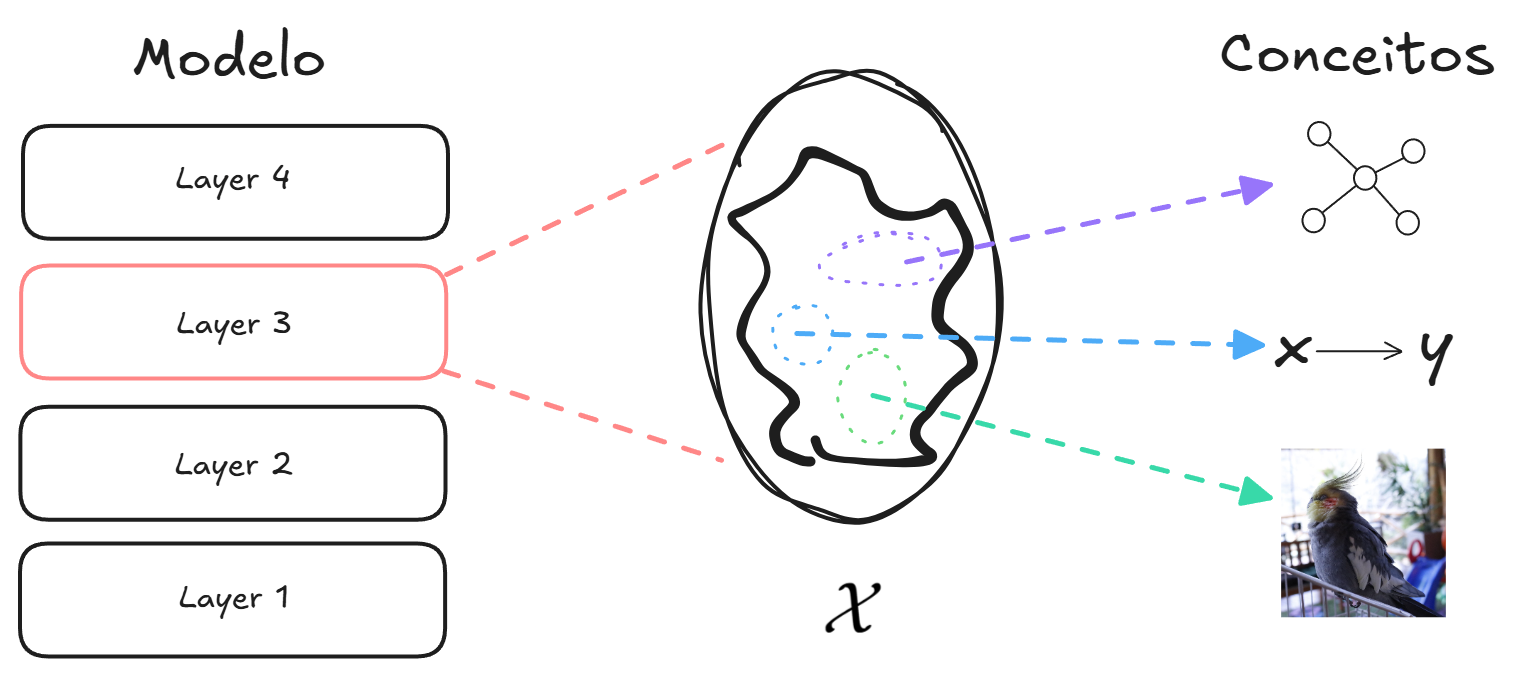
\includegraphics[width=\textwidth]{img/Concepts.png}
    \caption{Representação esquemática da extração de conceitos a partir de uma camada intermediária do modelo: a Layer 3 é projetada em um espaço latente, no qual diferentes regiões correspondem a conceitos distintos, associados tanto a estruturas abstratas quanto a padrões funcionais e semânticos.}
    \label{fig:concepts}
\end{figure}

Métodos geométricos de interpretabilidade, por sua vez, fundamentam-se na estrutura matemática dos espaços de representação internos dos modelos, utilizando ferramentas de geometria, teoria espectral e análise funcional para caracterizar o comportamento da rede. O \textit{geometric deep learning} fornece a base teórica dessa abordagem ao formalizar a aprendizagem profunda sobre domínios não euclidianos, como grafos e variedades \citep{Cao2020, Bronstein2017}. Nesse sentido, um modelo pode ser tratado como o próprio objeto geométrico a ser analisado, de modo que a geometria dos espaços de funções resultantes é utilizada para diagnosticar e explicar as decisões do modelo. A Figura \ref{fig:concepts} ilustra essa ideia de forma esquemática, em que a representação de uma camada intermediária é projetada em um espaço no qual regiões distintas correspondem a conceitos distintos.

\subsection{Um método de interpretabilidade baseado em \textit{kernels}}\label{subsec:metodo_proposto}

Este trabalho propõe um método geométrico de interpretabilidade baseado em \textit{kernels}. De acordo com a tipologia apresentada anteriormente, trata-se de um método \textit{post-hoc}, pois opera sobre um modelo já treinado sem interferir no seu treinamento, e modelo-agnóstico, pois a sua formulação exige apenas que cada amostra possa ser descrita por um conjunto de fontes de informação sobre as quais se define um \textit{kernel}, sem supor nenhuma arquitetura. A escolha das fontes, por sua vez, constitui uma instanciação do método, que pode utilizar estados internos de uma rede neural ou o caminho percorrido em uma árvore de decisão. O método produz explicações locais, sobre amostras e pares de amostras, e globais, sobre a organização do espaço de representação. Além disso, a distância que ele induz define quais instâncias são próximas, o que permite escolher contrafactuais e atribuir a diferença entre uma amostra e o seu contrafactual às variáveis de entrada. O método é descrito ao longo das próximas seções: o tensor de similaridade que o fundamenta é desenvolvido na Seção \ref{sec:tensor_rkhs}, o procedimento de construção da matriz de Gram é apresentado na Seção \ref{sec:kernel_pipeline} e a energia espectral utilizada em suas leituras é definida na Subseção \ref{subsec:spectral}.

Por fim, o método se diferencia das técnicas de análise representacional que também operam sobre matrizes de similaridade, como a análise de similaridade representacional (RSA) \citep{Kriegeskorte2008} e o alinhamento centrado de \textit{kernels} (CKA) \citep{Kornblith2019}. Essas técnicas são utilizadas para comparar representações, sejam elas de duas camadas, de dois modelos ou de um modelo e um sistema biológico, e resumem essa comparação em um único valor de semelhança. O método proposto, por sua vez, não tem como objetivo comparar representações, mas sim construir um espaço de representação a partir de fontes heterogêneas de um mesmo modelo e, a partir desse espaço, gerar afirmações sobre o comportamento do modelo que o originou. A relação formal entre o método e a CKA é examinada nos resultados.

\section{Núcleo Reprodutor em Espaços de Hilbert}\label{sec:rkhs}

O método proposto neste trabalho é construído sobre a teoria de \textit{kernels} formalizada por \cite{Aronszajn1950}, que faz parte da teoria clássica de aprendizagem de máquina. Os Espaços de Hilbert com Núcleo Reprodutor (\textit{Reproducing Kernel Hilbert Spaces} ou RKHS) fornecem a base funcional que conecta a noção de similaridade entre dados, expressa por \textit{kernels}, à geometria dos espaços de representação internos dos modelos. Ao garantir que a avaliação pontual de funções seja uma operação contínua, os RKHS permitem que propriedades geométricas do espaço de funções sejam exploradas de forma estável, o que é essencial para a construção de métodos de interpretabilidade que operem diretamente sobre as representações aprendidas. As definições apresentadas a seguir seguem \cite{Aronszajn1950} e \cite{Scholkopf2001}.

\textbf{Espaço de Hilbert:} Um espaço de Hilbert $\mathcal{H}$ é um espaço vetorial munido de um produto interno $\langle \cdot, \cdot \rangle_{\mathcal{H}}: \mathcal{H} \times \mathcal{H} \to \mathbb{R}$ que é completo em relação à norma induzida $\|f\|_{\mathcal{H}} = \sqrt{\langle f, f \rangle_{\mathcal{H}}}$. A completude significa que toda sequência de Cauchy, isto é, toda sequência cujos termos ficam arbitrariamente próximos entre si, converge para um elemento do próprio espaço, de modo que $\mathcal{H}$ não possui ``lacunas''.

\textbf{Núcleo Reprodutor:} Um núcleo reprodutor (\textit{kernel}) é uma função $k: \mathcal{X} \times \mathcal{X} \to \mathbb{R}$ simétrica, isto é, $k(x, x') = k(x', x)$ para todo $x, x' \in \mathcal{X}$, e positivamente definida, o que significa que, para qualquer conjunto finito de pontos $\{x_1, x_2, \dots, x_n\} \subset \mathcal{X}$ e quaisquer escalares $c_1, c_2, \dots, c_n \in \mathbb{R}$,

\begin{equation}\label{eq:pos_def}
    \sum_{i=1}^{n} \sum_{j=1}^{n} c_i \, c_j \, k(x_i, x_j) \geq 0.
\end{equation}

A exigência de definição positiva decorre diretamente da interpretação do \textit{kernel} como um produto interno em algum espaço de características. Considere um mapeamento $\phi: \mathcal{X} \to V$ tal que $k(x_i, x_j) = \langle \phi(x_i), \phi(x_j) \rangle_V$. A norma ao quadrado de um vetor $v = \sum_i c_i \, \phi(x_i) \in V$ é dada por

\begin{equation}\label{eq:kernel_norm}
    \|v\|^2 = \left\langle \sum_i c_i \, \phi(x_i),\; \sum_j c_j \, \phi(x_j) \right\rangle_V = \sum_{i=1}^{n} \sum_{j=1}^{n} c_i \, c_j \, k(x_i, x_j),
\end{equation}

\noindent de modo que a condição \eqref{eq:pos_def} equivale à não-negatividade da norma, propriedade necessária de qualquer produto interno. Na prática, calcular $\phi$ explicitamente pode ser inviável ou computacionalmente custoso. O \textit{kernel} contorna esse problema ao computar o produto interno no espaço transformado diretamente a partir dos pontos originais, sem jamais construir $\phi$ de forma explícita. Esse procedimento é conhecido como \textit{kernel trick} \citep{Scholkopf2001} e está ilustrado na Figura \ref{fig:kernel_trick}.

\begin{figure}[!htbp]
  \centering
  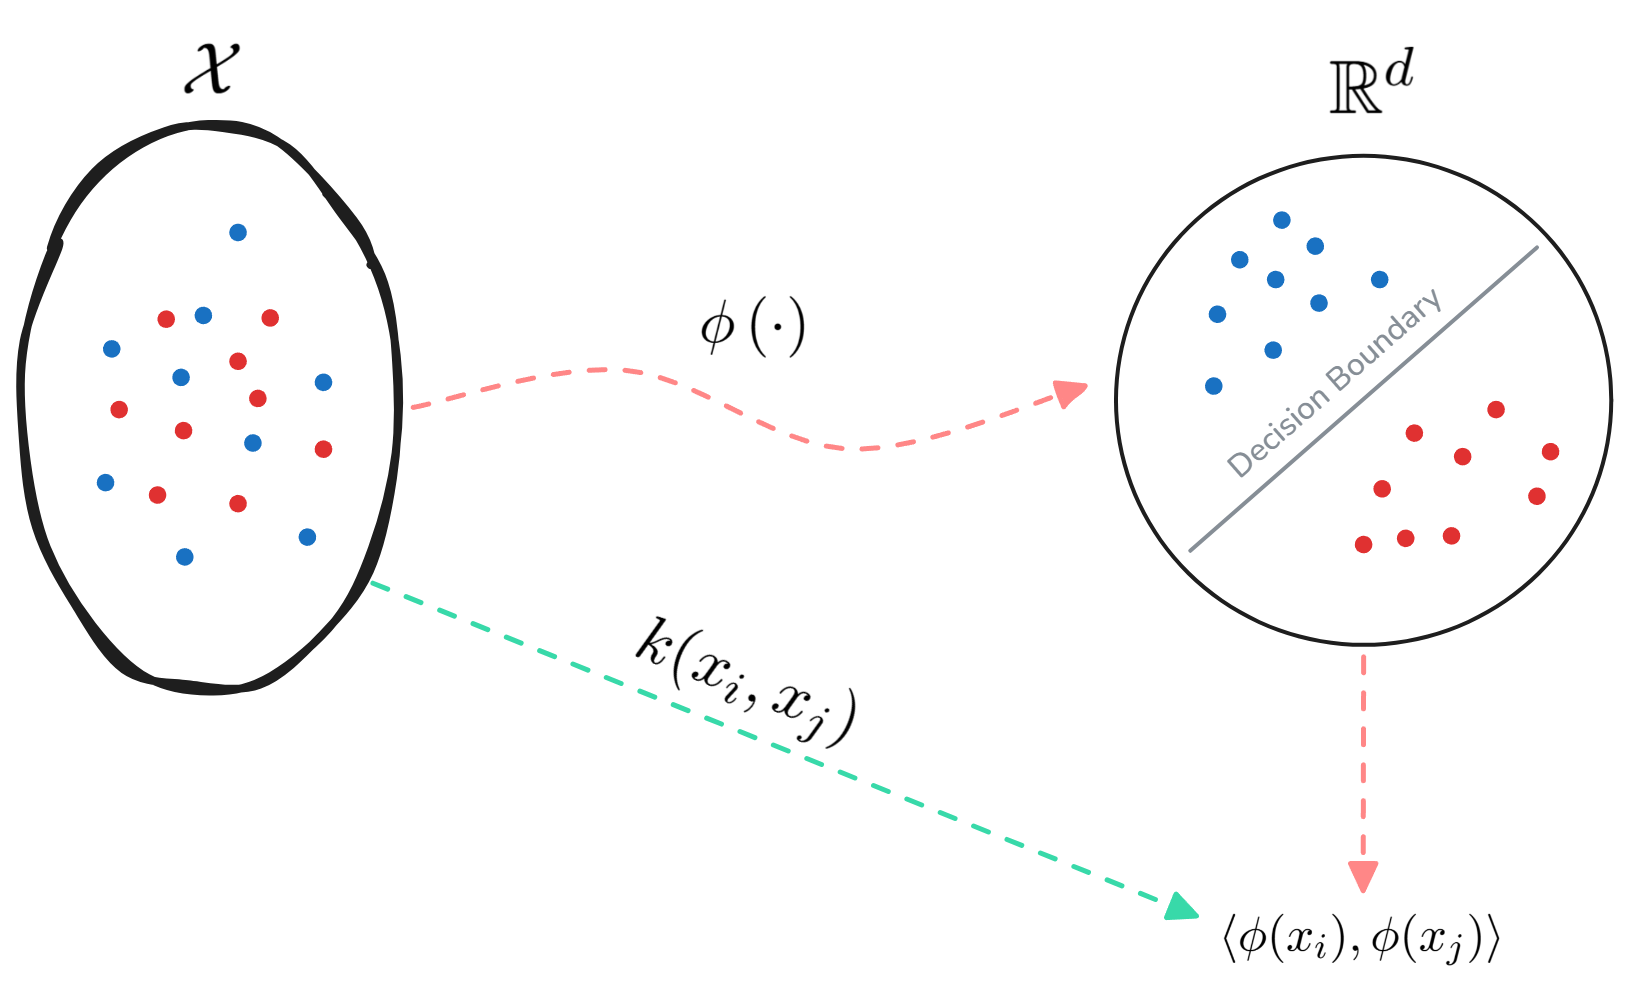
\includegraphics[width=\textwidth]{img/Kernel.png}
  \caption{O mapa de características $\phi$ leva os dados do espaço de entrada $\mathcal{X}$ para um espaço de dimensão maior $\mathbb{R}^d$\, onde as classes se tornam linearmente separáveis. Na prática, calcular $\phi$ explicitamente pode ser inviável ou computacionalmente custoso. O \textit{kernel} $k(x_i, x_j) = \langle \phi(x_i), \phi(x_j) \rangle$ contorna esse problema: ele computa o produto interno no espaço transformado diretamente a partir dos pontos originais, sem nunca construir $\phi$ (esse é o chamado ``\textit{kernel trick}'')}
  \label{fig:kernel_trick}
\end{figure}

\textbf{Matriz de Gram:}\label{def:gram} Dados $n$ pontos $\{x_1, x_2, \dots, x_n\} \subset \mathcal{X}$ e um \textit{kernel} $k$, a matriz de Gram é a matriz $K \in \mathbb{R}^{n \times n}$ cujas entradas são $K_{ij} = k(x_i, x_j)$. Pelo \textit{kernel trick}, cada entrada corresponde ao produto interno $\langle \phi(x_i), \phi(x_j) \rangle_V$ no espaço de características, de modo que $K$ codifica todas as relações de similaridade entre os pontos sem que $\phi(\cdot)$ precise ser obtido. A condição de definição positiva do \textit{kernel} garante que $K$ é semidefinida positiva, isto é, $c^\top K c \geq 0$ para todo $c \in \mathbb{R}^n$, que é a mesma condição imposta pelo produto interno expressa em formato matricial.

\textbf{Kernel Produto:} Dado um conjunto $\{k_1, k_2, \dots, k_n\}$ de \textit{kernels} positivamente definidos, com cada $k_i: \mathcal{X}_i \times \mathcal{X}_i \to \mathbb{R}$, o \textit{kernel} produto definido sobre $\mathcal{X} = \mathcal{X}_1 \times \mathcal{X}_2 \times \cdots \times \mathcal{X}_n$ é dado por

\begin{equation}\label{eq:kernel_prod}
    k(x, x') = \prod_{i=1}^{n} k_i(x_i, x_i'),
\end{equation}

\noindent onde $x = (x_1, \dots, x_n)$ e $x' = (x_1', \dots, x_n')$. Veja que, em termos matriciais, a matriz de Gram de $k$ é o produto de Hadamard $K_1 \circ K_2 \circ \cdots \circ K_n$ das matrizes de Gram dos fatores. Como o produto de Hadamard de matrizes semidefinidas positivas é semidefinido positivo, pelo teorema de Schur \citep{Schur1911, HornJohnson2013}, o \textit{kernel} produto também é positivamente definido.

\textbf{RKHS:} Um Espaço de Hilbert com Núcleo Reprodutor é um espaço de Hilbert $\mathcal{H}$ de funções $f: \mathcal{X} \to \mathbb{R}$ no qual existe um \textit{kernel} $k: \mathcal{X} \times \mathcal{X} \to \mathbb{R}$ tal que duas propriedades são satisfeitas: (1) para todo $x \in \mathcal{X}$, a função $k(\cdot, x)$ pertence a $\mathcal{H}$, (2) para toda $f \in \mathcal{H}$ e todo $x \in \mathcal{X}$,

\begin{equation}\label{eq:reproducing}
    f(x) = \langle f, \, k(\cdot, x) \rangle_{\mathcal{H}}.
\end{equation}

A Equação \eqref{eq:reproducing} é denominada propriedade reprodutora e dá nome ao espaço. Ela estabelece que avaliar uma função $f$ em um ponto $x$ equivale a tomar o produto interno de $f$ com a função \textit{kernel} ancorada em $x$, $k(\cdot, x)$. Uma consequência imediata é que o próprio \textit{kernel} pode ser recuperado pelo produto interno de duas dessas fatias:

\begin{equation}\label{eq:kernel_inner}
    k(x, x') = \langle k(\cdot, x), \, k(\cdot, x') \rangle_{\mathcal{H}}.
\end{equation}

A propriedade reprodutora implica, ainda, que o funcional de avaliação pontual $\delta_x: f \mapsto f(x)$ é um funcional linear contínuo em $\mathcal{H}$. Essa continuidade não é garantida em espaços de Hilbert arbitrários de funções e é precisamente o que distingue um RKHS de um espaço de Hilbert genérico \citep{Aronszajn1950}. A continuidade da avaliação pontual assegura que funções próximas na norma de $\mathcal{H}$ produzem valores próximos em cada ponto do domínio, conferindo estabilidade às representações no espaço e tornando o RKHS particularmente adequado para problemas de aprendizado em que se deseja controlar a complexidade das funções aprendidas e explorar a geometria do espaço de representação.

\textbf{Teorema de \cite{Aronszajn1950}:} Se $k: \mathcal{X} \times \mathcal{X} \to \mathbb{R}$ é simétrico e positivamente definido, então existe um único RKHS $\mathcal{H}_k$ cujo núcleo reprodutor é $k$. Reciprocamente, todo RKHS possui um único núcleo reprodutor.

\noindent A demonstração é construtiva: o espaço é gerado pelas combinações lineares finitas das funções $k(\cdot, x)$, com o produto interno definido pelo próprio \textit{kernel}, e completado pelos limites de suas sequências de Cauchy. Essa correspondência tem uma consequência direta para este trabalho, visto que, dado um conjunto de \textit{kernels} positivamente definidos $\{k_1, \dots, k_d\}$, cada um determina automaticamente seu próprio RKHS $\mathcal{H}_{k_1}, \dots, \mathcal{H}_{k_d}$.

\section{Trabalhos Relacionados}\label{sec:relacionados}

\cite{Graff2025} argumenta que, embora os métodos de XAI frequentemente sejam descritos como oferecendo ``razões" para as decisões de modelos de IA, essa caracterização é equivocada. O autor apresenta duas famílias de explicação por razão: causal/disposicional e interpretativa. Seu argumento é que nenhuma das duas famílias pode ser adequadamente aplicada a sistemas de IA. No primeiro caso, porque modelos de aprendizado de máquina não possuem atitudes normativas ou estados mentais que justifiquem suas decisões. No segundo, porque não é possível assumir que esses modelos possuam uma ``perspectiva" racional ou intencional que permita compreender suas ações em um ``sentido justificável". Assim, as explicações de XAI não são explicações por razões, mas sim explicações causais, que descrevem relações entre entradas e saídas sem envolver juízos normativos ou justificativos. O autor enfatiza as consequências práticas desse equívoco conceitual: ao apresentar as saídas de XAI como se fossem explicações de razões, corre-se o risco de criar falsas expectativas e uma confiança indevida nos sistemas de IA, levando usuários a acreditar que os modelos possuem justificativas racionais para suas recomendações. Em vez disso, defende que as explicações devem ser apresentadas em termos estritamente causais ou funcionais, evitando termos intencionais que sugerem agência ou racionalidade onde ela não existe. Esse diagnóstico reforça a necessidade de métodos que explicitem formalmente qual tipo de explicação está sendo gerado, em vez de tratarem todas as saídas de XAI como equivalentes.

Dando continuidade a essa discussão conceitual, o estudo de \cite{Pawlicki2024} aprofunda a lacuna epistemológica sob uma perspectiva metodológica, mostrando que a fragmentação não se limita ao conceito de explicação, mas também atinge os próprios critérios utilizados para avaliá-la. Através de uma revisão sistemática conduzida com rigor metodológico (PRISMA), os autores identificam um cenário marcado pela proliferação de propriedades, métricas e taxonomias que pretendem avaliar explicações em IA, mas que carecem de uniformidade terminológica, fundamentação conceitual comum e compatibilidade operacional. O estudo revela a existência de quase noventa métricas distintas utilizadas na literatura para mensurar ``qualidade explicativa", muitas delas redundantes, parcialmente sobrepostas ou introduzidas de forma idiossincrática por determinados grupos de pesquisa, o que torna inviável a comparação sistemática entre métodos de XAI. A contribuição mostra, assim, que o campo carece não apenas de uma definição clara do que conta como explicação, mas também de critérios sistemáticos e normativamente justificados para avaliar quando uma explicação é ``boa", ``adequada" ou ``suficiente".

Em uma proposta para minimizar sobreposições semânticas e agrupar diferentes terminologias que descreviam conceitos similares, \cite{Nauta2023} apresentou 12 propriedades, denominadas Co-12, para avaliar um sistema XAI. As Co-12 foram elencadas a partir de uma ampla revisão conceitual sobre qualidade de explicações, cobrindo tanto métodos \textit{ante-hoc} quanto \textit{post-hoc}, sendo o resultado um conjunto de propriedades categorizadas em três dimensões: conteúdo (\textit{correctness, completeness, consistency, continuity, contrastivity, covariate complexity}), apresentação (\textit{compactness, composition, confidence}) e usuário (\textit{context, coherence, controllability}). Somando a esse diagnóstico, \cite{Zhou2021} sistematiza métodos e métricas para avaliar explicações em ML e propõe uma base conceitual útil para comparar técnicas. O artigo distingue propriedades de interpretabilidade e de fidelidade, organiza explicadores em três classes (baseados em modelo, em atribuição e em exemplos) e descreve três eixos de avaliação. Um achado particularmente importante é o desbalanceamento no modo como a literatura avalia os explicadores: métodos baseados em modelo e em exemplos tendem a privilegiar critérios ligados à parcimônia e simplicidade estrutural, enquanto métodos baseados em atribuição concentram-se na fidelidade e na robustez. Essa assimetria ilustra como ainda há uma lacuna entre os esforços normativos, que descrevem o que deveria ser explicado, e os esforços técnicos, que medem o que de fato está sendo explicado, justificando a necessidade de uma visão integrada capaz de situar as propriedades de XAI dentro de estruturas explicativas consistentes em nível científico e não apenas operacional.

No contexto da interpretabilidade mecanicista em redes neurais com ativação ReLU, \cite{Barua2026} apresentam o método \textit{ReLU Region Reason} (Re3), que parte da propriedade de que essas redes se comportam de modo linear dentro de regiões específicas do espaço de entrada. Assim, para cada amostra, o método reescreve exatamente a computação da rede como um único mapeamento afim, \(f(x)=A_r x + D_r\), determinado pelos neurônios que permanecem ativos naquele caso. Isso permite calcular, de forma determinística e sem aproximações estocásticas, a contribuição exata de cada \textit{feature} nos \textit{logits} e nas probabilidades, além de identificar as regiões lineares em que a rede organiza o espaço de entrada. Os autores mostram alta concordância com LIME e SHAP nos rankings de importância, mas com estabilidade perfeita entre execuções. A relevância do Re3 está em mostrar que a geometria interna de redes ReLU pode ser explorada diretamente como mecanismo explicativo, aproximando-se de uma explicação causal-mecanicista ao reconstruir os caminhos computacionais efetivos de cada decisão.

\cite{Wickstrom2023} defende o método \textit{Representation Learning Explainability} (RELAX) como o primeiro método de explicação baseada em atribuição voltado especificamente para representações, e não para predições. A ideia central consiste em mascarar regiões da entrada e medir, via similaridade cosseno no espaço latente, o quanto a representação se altera, atribuindo importância às regiões cuja oclusão provoca maior mudança. O método é fundamentado teoricamente por uma interpretação em termos de \textit{kernels}: a importância de cada pixel corresponde a uma função de pontuação linear entre a representação original e a média ponderada das representações mascaradas no RKHS induzido pela função de similaridade. Além disso, o método incorpora quantificação de incerteza nas próprias explicações, permitindo filtrar regiões cuja atribuição é instável e aumentando a fidelidade do mapa de relevância resultante. A conexão explícita entre espaços de \textit{kernels} e atribuição de importância constitui um precedente direto para o presente trabalho, que estende essa lógica ao compor, por meio do produto tensorial de RKHS, matrizes de Gram construídas a partir de múltiplas fontes de um mesmo modelo, das quais os pesos, as ativações e os gradientes utilizados nos experimentos são apenas uma instanciação.

De forma complementar, \cite{Mae2026} propõem um arcabouço baseado em análise espectral para investigar a estrutura da qualidade de explicações em XAI. Os autores aplicam a decomposição em valores singulares (SVD) a uma matriz de redistribuição que codifica a atribuição de cada neurônio de saída a cada \textit{feature} de entrada, e demonstram que os valores singulares dessa matriz revelam dois fatores fundamentais da qualidade explicativa: estabilidade e sensibilidade ao alvo. A estabilidade é controlada pelo maior valor singular \(\sigma_1\) da matriz de redistribuição, que limita a amplificação de ruído durante o processo de explicação, enquanto a sensibilidade é capturada pela norma do espectro completo \(\|\sigma\|_2\), que mede a capacidade da explicação de distinguir entre diferentes conceitos na saída. Os autores mostram que esses dois fatores estão em tensão: parâmetros que aumentam a estabilidade tendem a reduzir a sensibilidade, e vice-versa, e propõem uma métrica combinada (SSM) que identifica o ponto de equilíbrio entre ambos. A relevância desse trabalho para o presente estudo reside em dois pontos. Primeiro, ele demonstra que a análise espectral é uma ferramenta poderosa para diagnosticar propriedades estruturais de explicações, o que corrobora a escolha da decomposição espectral de matrizes de Gram como operação central do arcabouço aqui proposto. Segundo, ao identificar estabilidade e sensibilidade como fatores espectralmente observáveis, ele oferece um vocabulário formal que se conecta à decomposição da energia espectral utilizada neste trabalho (Subseção \ref{subsec:spectral}), em que a energia retida nos modos dominantes, \(\widehat{E}_{\parallel}\), concentra as direções que organizam o espaço de representação, e a energia ortogonal, \(\widehat{E}_{\perp}\), isola aquilo que o subespaço retido não representa.

No campo da aprendizagem de representações, o trabalho de \cite{Dean2025} propõe um arcabouço matemático formal para descrever as transformações do mundo a partir da perspectiva de um agente em contextos de aprendizagem por reforço. Os autores partem do formalismo de representações \textit{disentangled} baseadas em simetria (SBDRL), que pressupõe que as simetrias do mundo devem estar presentes na representação interna do agente. Entretanto, demonstram que essa abordagem é restritiva, pois não consegue capturar transformações comuns em cenários de aprendizagem por reforço, como ações irreversíveis (por exemplo, consumir um item), ações restritas por obstáculos (paredes) ou mundos com ações não homogêneas. Para superar essas limitações, os autores generalizam tanto a condição de equivariância quanto a definição de \textit{disentanglement} do SBDRL utilizando teoria das categorias, estendendo-as de estruturas de grupo para qualquer álgebra, incluindo monoides e categorias pequenas. A relevância desse trabalho para o presente estudo reside na demonstração de que as propriedades de transformação do mundo podem ser formalizadas em estruturas algébricas mais gerais, o que se conecta diretamente com a proposta de utilizar a geometria dos espaços de representação como base para a interpretabilidade mecanicista, visto que tanto a abordagem algébrica quanto a geométrica buscam caracterizar as invariâncias e equivariâncias que organizam as representações internas dos modelos.

Os trabalhos revisados revelam três lacunas que o presente estudo pretende endereçar. Do ponto de vista conceitual, \cite{Graff2025} e \cite{Erasmus2021} mostram que o campo de XAI carece de clareza sobre qual tipo de explicação científica (dedutiva, indutiva, causal) está sendo gerado, e que essa distinção tem consequências práticas diretas para a confiança e a responsabilização. Do ponto de vista avaliativo, \cite{Pawlicki2024}, \cite{Nauta2023} e \cite{Zhou2021} evidenciam que as métricas existentes capturam dimensões distintas e por vezes incompatíveis da qualidade explicativa, sem um arcabouço unificador. Do ponto de vista técnico, os métodos geométricos e espectrais existentes, como o Re3 \citep{Barua2026}, o RELAX \citep{Wickstrom2023} e a análise espectral de redistribuição de \cite{Mae2026}, demonstram que a estrutura geométrica e espectral das representações internas contém informação explicativa rica, mas cada um deles opera sobre uma única fonte de informação e sobre uma construção específica, sem um arcabouço formal que garanta, para qualquer combinação de fontes, a existência de um espaço de representação com geometria e espectro bem definidos.

O presente trabalho responde a essas lacunas em dois níveis. No nível teórico, que constitui a sua principal contribuição, ele propõe o tensor de similaridade em RKHS e o pipeline núcleo-transformação, que compõem fontes heterogêneas de um mesmo modelo em um único espaço de representação e garantem, por demonstração, a semidefinição positiva, a pseudométrica e a decomposição da energia espectral sobre as quais as leituras são feitas, quaisquer que sejam as fontes e os \textit{kernels} escolhidos. Veja que essa construção é modelo-agnóstica, e os resultados mostram que ela se aplica, sem alteração, a um perceptron multicamadas, a uma rede convolucional, a um transformador e a uma árvore de decisão. No nível empírico, o trabalho responde à lacuna avaliativa com um protocolo em que cada leitura é formulada como uma pergunta sobre o comportamento do modelo (Subseção \ref{subsec:perguntas}), respondida contra uma referência externa à geometria e acompanhada de uma referência de nulidade construída para ela. Por fim, responde à lacuna conceitual declarando o tipo de explicação que cada leitura produz: as leituras de vizinhança, de erro e de confusão descrevem o comportamento do modelo, enquanto a leitura de diferenças entre uma amostra e o seu contrafactual e a datação são validadas por intervenção sobre a entrada ou sobre os estados internos, o que as aproxima da explicação causal-intervencionista e contrafactual discutida na Seção \ref{sec:referencial}.

\section{Tensor de Similaridade em Espaços de Hilbert com Núcleo Reprodutor}\label{sec:tensor_rkhs}

A Seção \ref{sec:rkhs} estabeleceu os fundamentos dos RKHS, demonstrando que todo \textit{kernel} simétrico e positivamente definido determina um único RKHS, e que o produto de \textit{kernels} positivamente definidos é também positivamente definido. Esta seção desenvolve, sobre esses fundamentos, a base matemática do método proposto, isto é, o tensor de similaridade construído via produto tensorial de RKHS, e os seus resultados, junto com os das Seções \ref{sec:kernel_pipeline} e \ref{sec:representation_geometry}, constituem a principal contribuição deste trabalho. A construção é apresentada em quatro etapas: o produto tensorial de espaços de Hilbert, o tensor de similaridade como núcleo reprodutor do produto tensorial, a estrutura métrica via curvas de nível, e o complemento ortogonal de RKHS. Cada etapa é fundamentada por demonstrações dos resultados centrais, sem referência a aplicações específicas. Observe que nenhum desses resultados depende de quais são as $d$ fontes ou de quais \textit{kernels} são utilizados, sendo exigido apenas que cada $k_l$ seja positivamente definido. A forma como essa teoria é aplicada sobre uma amostra finita é apresentada na Seção \ref{sec:kernel_pipeline}, enquanto a instanciação utilizada nos experimentos é apresentada na Seção \ref{sec:metodologia}.

\subsection{Produto Tensorial de Espaços de Hilbert}

A questão central que motiva esta construção é a seguinte: dados $d$ espaços de Hilbert independentes, cada um codificando uma forma de similaridade sobre um mesmo conjunto $\mathcal{X}$, como construir um espaço único que codifique todas as similaridades simultaneamente, de tal modo que a estrutura de produto interno seja preservada? A resposta é fornecida pelo produto tensorial.

\textbf{Tensor Elementar:} Sejam $\mathcal{H}_1, \mathcal{H}_2, \dots, \mathcal{H}_d$ espaços de Hilbert. Um tensor elementar é um objeto da forma $f_1 \otimes f_2 \otimes \cdots \otimes f_d$, com $f_l \in \mathcal{H}_l$ para cada $l \in \{1, \dots, d\}$. O símbolo $\otimes$ é multilinear, isto é, para quaisquer escalares $\alpha, \beta \in \mathbb{R}$ e quaisquer $f_l, g_l \in \mathcal{H}_l$:

\begin{equation}\label{eq:tensor_multilinear}
    f_1 \otimes \cdots \otimes (\alpha f_l + \beta g_l) \otimes \cdots \otimes f_d = \alpha (f_1 \otimes \cdots \otimes f_l \otimes \cdots \otimes f_d) + \beta (f_1 \otimes \cdots \otimes g_l \otimes \cdots \otimes f_d).
\end{equation}

O tensor elementar não é uma soma nem um produto ordinário de funções. Ele é um objeto que vive em um espaço novo e representa uma interação multilinear entre os fatores $f_1, \dots, f_d$. Sua decomposição em fatores não é única, pois diferentes reescalonamentos podem representar o mesmo tensor, mas a estrutura conjunta definida por esses fatores é preservada no produto tensorial.

\textbf{Produto Tensorial de Espaços de Hilbert:} Considere o espaço vetorial das combinações lineares finitas de tensores elementares,

\begin{equation}\label{eq:tensor_space}
    \mathcal{T}_0 = \left\{ \sum_{m=1}^{N} c_m \, f_1^{(m)} \otimes f_2^{(m)} \otimes \cdots \otimes f_d^{(m)} \, : \, N \in \mathbb{N}, \, c_m \in \mathbb{R}, \, f_l^{(m)} \in \mathcal{H}_l \right\},
\end{equation}

\noindent modulado pelas relações de multilinearidade \eqref{eq:tensor_multilinear}. Sobre $\mathcal{T}_0$ define-se uma forma bilinear simétrica

\begin{equation}\label{eq:tensor_inner}
    \left\langle \bigotimes_{l=1}^{d} f_l, \; \bigotimes_{l=1}^{d} g_l \right\rangle = \prod_{l=1}^{d} \langle f_l, g_l \rangle_{\mathcal{H}_l},
\end{equation}

\noindent estendida por bilinearidade às combinações lineares finitas. O produto tensorial algébrico $\mathcal{T}_0 = \bigotimes_{l=1}^{d} \mathcal{H}_l$ é então o espaço de Hilbert definido como o completamento com respeito à norma $\|u\| = \sqrt{\langle u,u \rangle}$.

A consequência crucial expressa por \eqref{eq:tensor_inner} é que o produto interno no espaço tensorial se fatora: a similaridade entre dois tensores elementares é o produto das similaridades componente a componente. Esta propriedade é a base de todos os resultados subsequentes desta seção.

\begin{proposition}[Produto interno bem definido e positivo definido]\label{prop:inner_well_defined}
A forma bilinear definida em \eqref{eq:tensor_inner} estende-se por bilinearidade a um produto interno bem definido, simétrico e positivo definido sobre o produto tensorial algébrico $\mathcal{T}_0 = \bigotimes_{l=1}^{d} \mathcal{H}_l$.
\end{proposition}

\begin{proof}
A bilinearidade e a simetria decorrem diretamente das propriedades dos produtos internos em cada espaço componente $\mathcal{H}_l$. Para verificar a positividade, considere $u = \sum_{m} c_m \bigotimes_{l} f_l^{(m)} \in \mathcal{T}_0$. Pela bilinearidade, $\langle u,u\rangle = \sum_{m} \sum_{n} c_m c_n \prod_{l} \left\langle f_l^{(m)},f_l^{(n)} \right\rangle_{\mathcal{H}_l}$. Para cada $l$, seja $E_l = \operatorname{span} \left\{f_l^{(1)},\dots,f_l^{(N)} \right\} \subseteq \mathcal{H}_l$.

\noindent Como $E_l$ é finito-dimensional, escolha uma base ortonormal $\{e_{l,1},\dots,e_{l,r_l}\}$ de $E_l$. Então $u$ pode ser escrito de maneira única na forma

\begin{equation*}
    u = \sum_{i_1=1}^{r_1} \cdots \sum_{i_d=1}^{r_d} a_{i_1,\dots,i_d}\, e_{1,i_1}\otimes\cdots\otimes e_{d,i_d}.
\end{equation*}

\noindent Pela definição do produto interno tensorial e pela ortonormalidade das bases, os tensores $e_{1,i_1}\otimes\cdots\otimes e_{d,i_d}$ são ortonormais. Consequentemente,

\begin{equation*}
    \langle u,u\rangle = \sum_{i_1=1}^{r_1} \cdots \sum_{i_d=1}^{r_d} |a_{i_1,\dots,i_d}|^2 \geq 0.
\end{equation*}

\noindent Além disso, $\langle u,u\rangle=0$ se e somente se todos os coeficientes $a_{i_1,\dots,i_d}$ são nulos, isto é, se e somente se $u=0$. Portanto, a forma é positiva definida e constitui um produto interno sobre $\mathcal{T}_0$.
\end{proof}

\begin{remark}[Dimensionalidade do produto tensorial]\label{rem:tensor_dim}
Quando cada $\mathcal{H}_l$ tem dimensão finita $D_l$, o produto tensorial $\bigotimes_{l=1}^{d} \mathcal{H}_l$ tem dimensão $\prod_{l=1}^{d} D_l$. As dimensões se multiplicam, não se somam. Em termos geométricos, isso reflete o fato de que um par de bases $\{e_i^{(1)}\}$ e $\{e_j^{(2)}\}$ de dois espaços $\mathcal{H}_1$ e $\mathcal{H}_2$ gera uma base $\{e_i^{(1)} \otimes e_j^{(2)}\}$ de $\mathcal{H}_1 \otimes \mathcal{H}_2$ cuja cardinalidade é $D_1 \cdot D_2$. Cada par de direções de cada espaço componente gera uma direção independente no espaço produto, conforme ilustrado na Figura \ref{fig:tensor_product}.
\end{remark}

\begin{figure}[htbp]
    \centering
    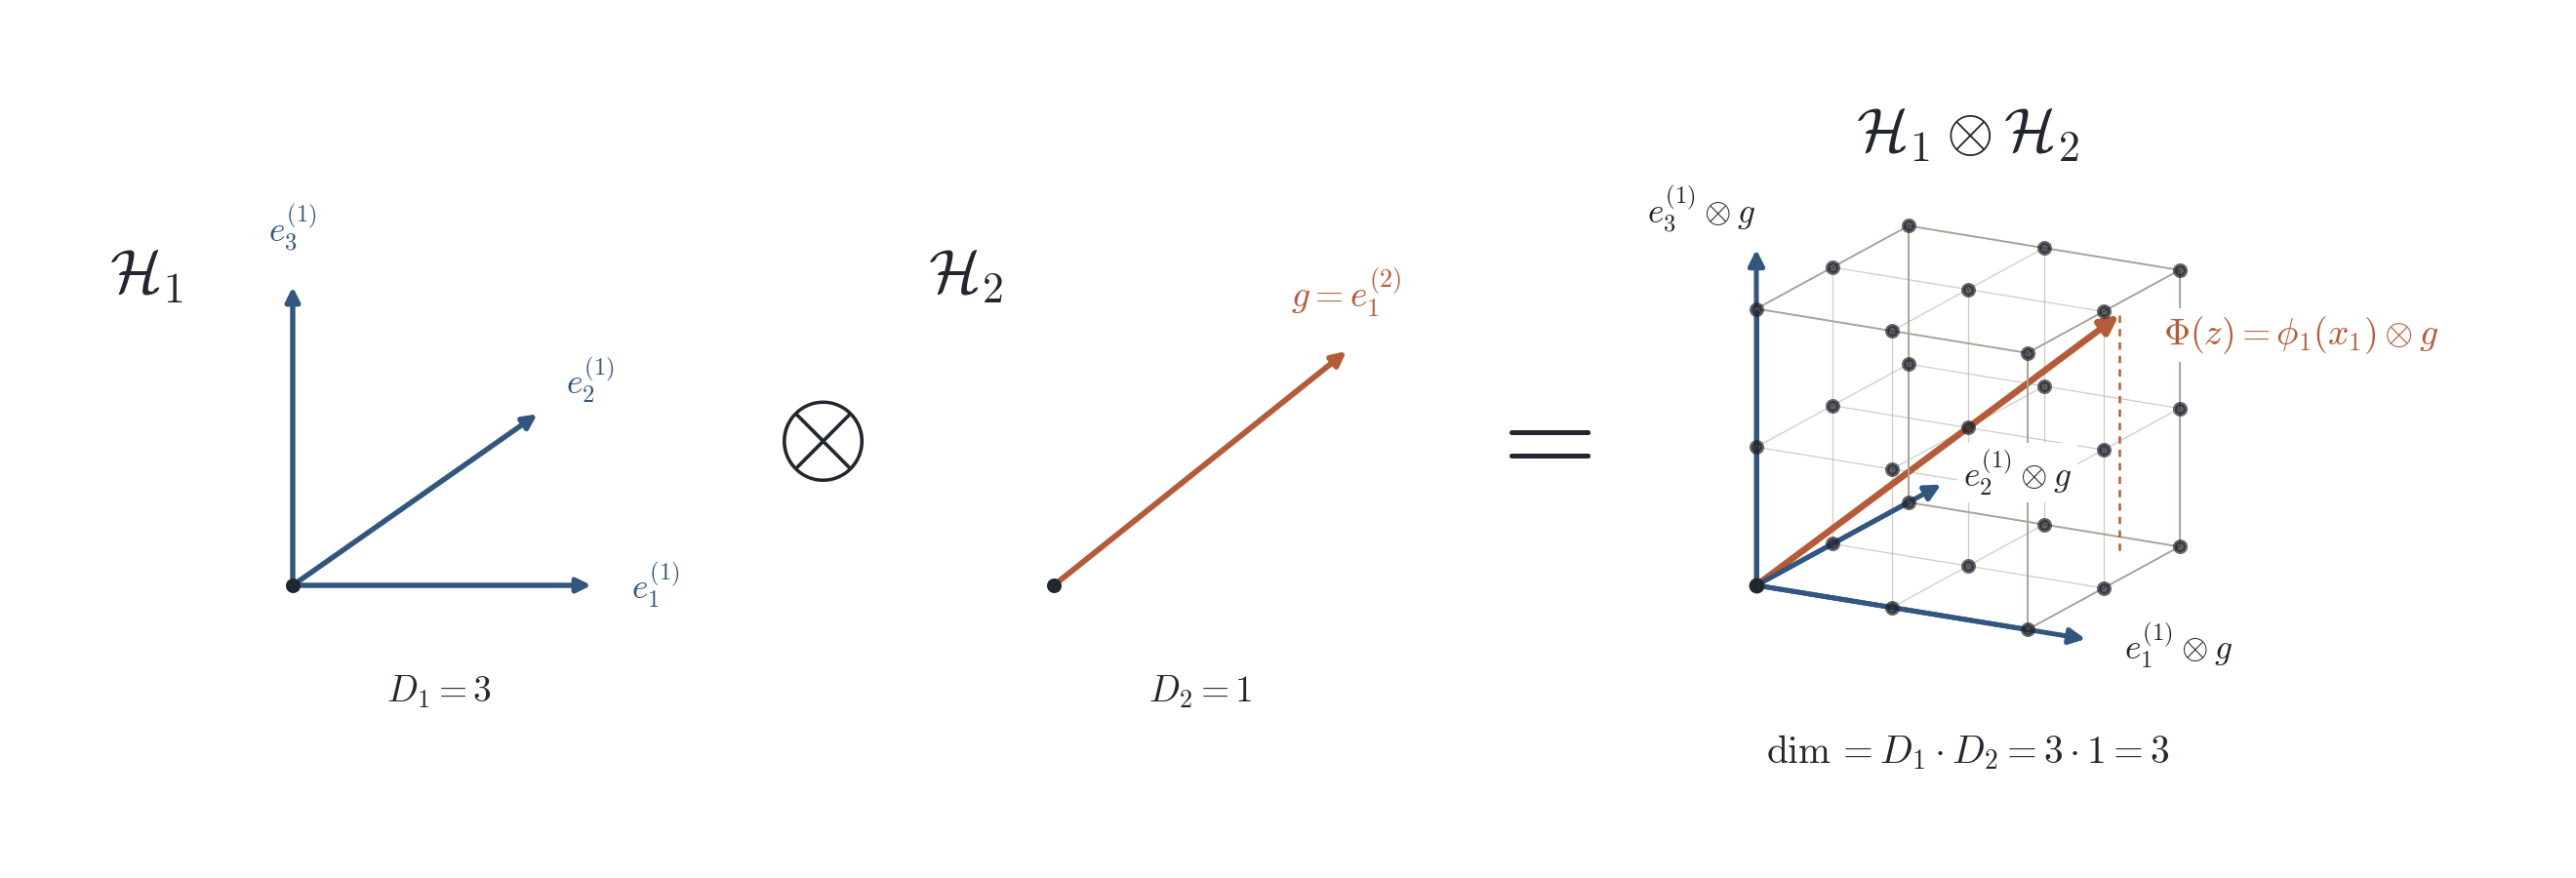
\includegraphics[width=\textwidth]{img/tensor_product_draft}
    \caption{Ilustração do produto tensorial $\mathcal{H}_1 \otimes \mathcal{H}_2$. Cada vetor da base $\{e_i^{(1)}\}$ de $\mathcal{H}_1$, com $D_1 = 3$, combinado ao vetor $g = e_1^{(2)}$ de $\mathcal{H}_2$, com $D_2 = 1$, gera uma direção $e_i^{(1)} \otimes g$ do espaço produto, cuja dimensão é $D_1 \cdot D_2 = 3$. O tensor de similaridade $\Phi(z) = \phi_1(x_1) \otimes g$ é um elemento desse espaço.}
    \label{fig:tensor_product}
\end{figure}

\subsection{Tensor de Similaridade sobre o Domínio Produto}
 
O objeto de análise deste trabalho não é um ponto de um domínio único, mas uma \emph{tupla} de fontes de informação. Sejam $\mathcal{X}_1, \dots, \mathcal{X}_d$ os domínios das $d$ fontes, cada um munido de um \textit{kernel} positivamente definido $k_l$, com RKHS $\mathcal{H}_{k_l}$ e mapa de características canônico $\phi_l(x_l) = k_l(\cdot, x_l)$. A unidade analisada vive no domínio produto
\begin{equation}\label{eq:product_domain}
    \mathcal{Z} = \mathcal{X}_1 \times \mathcal{X}_2 \times \cdots \times \mathcal{X}_d.
\end{equation}
 
\begin{definition}[Tensor de similaridade]\label{def:tensor_sim}
Para uma observação $z = (x_1, \dots, x_d) \in \mathcal{Z}$, o \emph{tensor de similaridade} é a representação tensorial
\begin{equation}\label{eq:tensor_sim_def}
    \Phi(z) = \phi_1(x_1) \otimes \cdots \otimes \phi_d(x_d) = \bigotimes_{l=1}^{d} \phi_l(x_l) \; \in \; \bigotimes_{l=1}^{d} \mathcal{H}_{k_l},
\end{equation}
cujo produto interno é dado pelo \textit{kernel} produto sobre $\mathcal{Z}$,
\begin{equation}\label{eq:tensor_sim_inner}
    K(z, z') = \langle \Phi(z), \Phi(z') \rangle = \prod_{l=1}^{d} \langle \phi_l(x_l), \phi_l(x_l') \rangle_{\mathcal{H}_{k_l}} = \prod_{l=1}^{d} k_l(x_l, x_l'),
\end{equation}
\noindent com $z = (x_1,\dots,x_d)$ e $z' = (x_1',\dots,x_d')$.

\end{definition}
 
\textbf{O tensor é implícito, a Gram o representa.} O tensor de similaridade $\Phi(z)$ é um objeto implícito, em geral de dimensão elevada ($\prod_l D_l$), que não precisa ser exibido explicitamente para que a estrutura de $\mathcal{H}_K$ seja acessível. Toda a informação relevante sobre um conjunto finito $\{z_1, \dots, z_n\}$, com $z_i = (x_{i1}, \dots, x_{id})$, reside nos produtos internos $\langle \Phi(z_i), \Phi(z_j)\rangle$, reunidos na \emph{matriz de Gram} $\mathbf{G}$. Por \eqref{eq:tensor_sim_inner}, essa matriz é o produto de Hadamard das Gram componentes:
\begin{equation}\label{eq:tensor_sim_gram}
    G_{ij} = \prod_{l=1}^{d} k_l(x_{il}, x_{jl}), \hspace{0.2cm} \text{isto é,} \hspace{0.2cm} \mathbf{G} = \mathbf{K}_1 \circ \mathbf{K}_2 \circ \cdots \circ \mathbf{K}_d, \quad (\mathbf{K}_l)_{ij} = k_l(x_{il}, x_{jl}).
\end{equation}
A matriz $\mathbf{G}$ é, assim, a realização finita do tensor de similaridade sobre a amostra: os objetos que caracterizam $\mathcal{H}_K$ se exprimem por meio dela, e não pelos tensores. A Figura \ref{fig:gram_hadamard} ilustra essa composição para $d = 3$ componentes.

\begin{figure}[htbp]
    \centering
    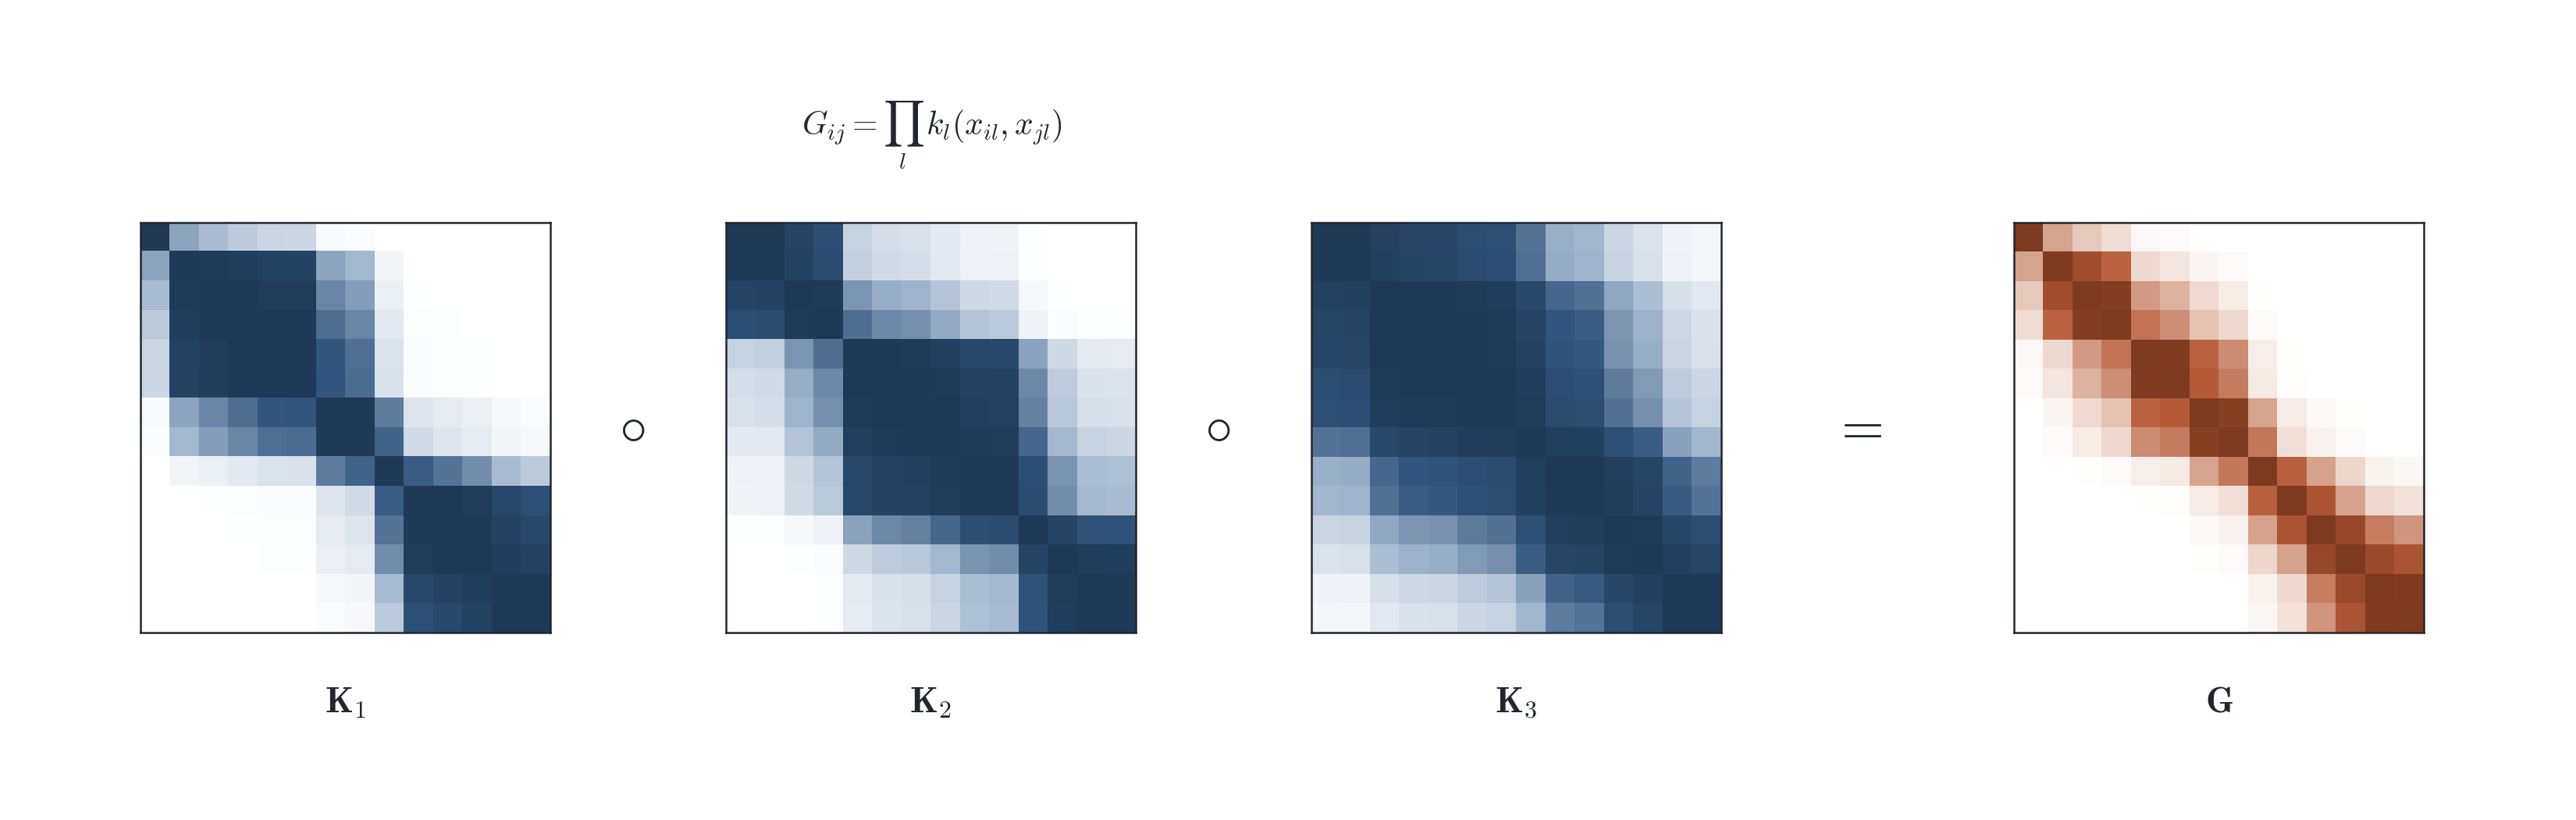
\includegraphics[width=\textwidth]{img/gram_hadamard_draft.png}
    \caption{Ilustração da matriz de Gram do tensor de similaridade como produto de Hadamard das matrizes de Gram componentes, $G_{ij} = \prod_l k_l(x_{il}, x_{jl})$. Veja que a matriz $\mathbf{G}$ só apresenta valores altos nas regiões em que as três componentes $\mathbf{K}_1$, $\mathbf{K}_2$ e $\mathbf{K}_3$ são simultaneamente altas, o que reflete o critério de similaridade conjunta do Comentário \ref{rem:joint_similarity}.}
    \label{fig:gram_hadamard}
\end{figure}
 
A escolha de trabalhar sobre o domínio produto $\mathcal{Z}$, e não sobre um domínio único com os fatores avaliados no mesmo ponto, é o que garante a forma limpa do teorema a seguir: como cada componente $x_l$ varia independentemente em $\mathcal{X}_l$, o tensor de similaridade percorre \emph{todos} os tensores elementares, e não apenas os diagonais.

 
\begin{theorem}[Realização do tensor de similaridade em RKHS]\label{thm:tensor_similarity}
Sejam $\mathcal{H}_{k_1}, \dots, \mathcal{H}_{k_d}$ RKHS com núcleos $k_1, \dots, k_d$ sobre domínios $\mathcal{X}_1, \dots, \mathcal{X}_d$, e seja $K$ o \textit{kernel} produto sobre $\mathcal{Z} = \prod_l \mathcal{X}_l$ definido por
\begin{equation}\label{eq:K_thm}
    K(z, z') = \prod_{l=1}^{d} k_l(x_l, x_l'), \qquad z = (x_1,\dots,x_d), \; z' = (x_1',\dots,x_d').
\end{equation}
Então $K$ é positivamente definido, e seu RKHS $\mathcal{H}_K$ é canonicamente isométrico ao produto tensorial \emph{completo},
\begin{equation}\label{eq:full_iso}
    \mathcal{H}_K \;\cong\; \bigotimes_{l=1}^{d} \mathcal{H}_{k_l},
\end{equation}
sob a identificação $\Phi(z) \mapsto K(\cdot, z)$.
\end{theorem}
 
\begin{proof}
A demonstração tem três passos.
 
\noindent \textit{(i) $K$ é positivamente definido.} Pela Equação \eqref{eq:kernel_prod} (Seção \ref{sec:rkhs}), o produto de \textit{kernels} positivamente definidos é positivamente definido, pelo Teorema de \cite{Aronszajn1950}, $K$ determina um único RKHS, denotado $\mathcal{H}_K$.
 
\noindent \textit{(ii) $\Phi$ preserva o produto interno.} Cada fator $\phi_l(x_l) = k_l(\cdot, x_l)$ pertence a $\mathcal{H}_{k_l}$, de modo que $\Phi(z)$ é um tensor elementar legítimo. Por \eqref{eq:tensor_inner} e pela propriedade reprodutora em cada fator,
\begin{equation*}
    \langle \Phi(z), \Phi(z') \rangle_{\bigotimes \mathcal{H}_{k_l}}
\end{equation*}
\begin{equation*}
    = \prod_{l=1}^{d} \langle k_l(\cdot, x_l), k_l(\cdot, x_l') \rangle_{\mathcal{H}_{k_l}}
\end{equation*}
\begin{equation*}
    = \prod_{l=1}^{d} k_l(x_l, x_l') = K(z, z') = \langle K(\cdot, z), K(\cdot, z') \rangle_{\mathcal{H}_K}.
\end{equation*}
Logo o mapa $\Phi(z) \mapsto K(\cdot, z)$, estendido por linearidade ao span dos tensores de similaridade, preserva o produto interno, é uma isometria linear.
 
\noindent \textit{(iii) Densidade nos dois lados.} Por definição de RKHS, o span de $\{K(\cdot, z) : z \in \mathcal{Z}\}$ é denso em $\mathcal{H}_K$. Reciprocamente, como cada $x_l$ varia \emph{independentemente} em $\mathcal{X}_l$ e o span de $\{k_l(\cdot, x_l)\}$ é denso em $\mathcal{H}_{k_l}$, a multilinearidade e a continuidade de $\otimes$ garantem que o span de $\{\Phi(z)\}$ seja denso em $\bigotimes_l \mathcal{H}_{k_l}$. Uma isometria definida num subespaço denso estende-se de modo único, por continuidade, a uma isometria \emph{sobrejetora} entre os fechos, obtém-se assim o isomorfismo \eqref{eq:full_iso}. A variação independente dos $x_l$ é o passo decisivo: sem ela, o span conteria apenas tensores diagonais e não seria denso (Comentário \ref{rem:diagonal_case}).
\end{proof}
 
\begin{remark}[Caso diagonal e suporte dos dados]\label{rem:diagonal_case}
A hipótese decisiva do Teorema \ref{thm:tensor_similarity} é a variação independente das componentes. Se, em vez disso, as $d$ fontes forem todas derivadas de um mesmo objeto subjacente $x$, por um mapa de acoplamento $x \mapsto (x_1(x), \dots, x_d(x))$, as observações vivem numa subvariedade acoplada de $\mathcal{Z}$ (o ``caso diagonal''), e o span de $\{\Phi\}$ gera apenas um subespaço \emph{próprio} de $\bigotimes_l \mathcal{H}_{k_l}$. Nesse regime, ainda que o isomorfismo \eqref{eq:full_iso} descreva o objeto no nível do domínio, a dimensão \emph{efetiva} suportada pelas observações satisfaz $\mathrm{rank}(\mathbf{G}) \leq n$, em geral abaixo de $\prod_l D_l$: é uma propriedade do suporte amostral, não do núcleo, e não afeta o teorema nem a forma da Gram $\mathbf{G} = \mathbf{K}_1 \circ \cdots \circ \mathbf{K}_d$.
\end{remark}
 
\begin{corollary}[Forma matricial]\label{cor:hadamard_form}
Sejam $\{z_1, \dots, z_n\} \subset \mathcal{Z}$ um conjunto finito e $\mathbf{K}_l$ a matriz de Gram de $k_l$ nas $l$-ésimas componentes. A matriz de Gram do \textit{kernel} produto é o produto de Hadamard $\mathbf{G} = \mathbf{K}_1 \circ \cdots \circ \mathbf{K}_d$, simétrica e semidefinida positiva.
\end{corollary}
 
\begin{proof}
A entrada $(i,j)$ de $\mathbf{K}_1 \circ \cdots \circ \mathbf{K}_d$ é $\prod_l (\mathbf{K}_l)_{ij} = \prod_l k_l(x_{il}, x_{jl}) = K(z_i, z_j)$. A simetria é preservada pelo produto de Hadamard de matrizes simétricas, e a semidefinição positiva decorre do teorema de Schur \citep{Schur1911, HornJohnson2013}.
\end{proof}
 

\begin{remark}[Critério de similaridade conjunta]\label{rem:joint_similarity}
A forma multiplicativa de \eqref{eq:K_thm} impõe um critério de similaridade \emph{conjunta}: assumindo $k_l \geq 0$ (como em \textit{kernels} normalizados), para que $K(z, z')$ seja grande é necessário que todo $k_l(x_l, x_l')$ seja grande. Um único fator próximo de zero suprime o produto, como pode ser observado na Figura \ref{fig:gram_hadamard}. Isso difere qualitativamente de uma combinação aditiva $\sum_l \alpha_l k_l$, em que um fator dominante poderia mascarar a discordância dos demais. Quando os $k_l$ podem ser negativos, a interpretação exige cuidado, pois cancelamentos de sinal podem produzir $K(z,z')$ pequeno mesmo com fatores individuais não pequenos em módulo.
\end{remark}

\begin{corollary}[Composição recursiva]\label{cor:recursive_composition}
Sejam $\mathcal{H}_{K^{(1)}}, \dots, \mathcal{H}_{K^{(L)}}$ RKHS, cada um já construído como o RKHS de um \textit{kernel} produto via Teorema \ref{thm:tensor_similarity}. Então o RKHS do \textit{kernel} produto $K_{\mathrm{tot}} = \prod_{\ell=1}^{L} K^{(\ell)}$ é canonicamente isométrico a $\bigotimes_{\ell=1}^{L} \mathcal{H}_{K^{(\ell)}}$.
\end{corollary}

\begin{proof}
Aplicação iterada do Teorema \ref{thm:tensor_similarity}, tomando os RKHS $\mathcal{H}_{K^{(\ell)}}$ como espaços componentes.
\end{proof}

A composição em níveis hierárquicos preserva, assim, a estrutura de RKHS: o \textit{kernel} total é o produto dos \textit{kernels} de nível, e o objeto que o realiza é novamente um tensor de similaridade. Essa propriedade permite estender o método descrito na Seção \ref{sec:kernel_pipeline} a níveis hierárquicos, como a composição entre camadas de um modelo construída sobre o produto tensorial entre fontes dentro de cada camada. Entretanto, essa extensão não é explorada na instanciação apresentada na Seção \ref{sec:metodologia}, que analisa cada camada separadamente.

\subsection{Estrutura Métrica via Curvas de Nível}\label{subsec:metric}
 
Estabelecida a realização de $\mathcal{H}_K$, resta dotá-lo de uma estrutura métrica utilizável. A estrutura natural é a distância induzida pela norma de $\mathcal{H}_K$.
 
\textbf{Distância no RKHS.} Seja $\Phi(z) = K(\cdot, z)$ o mapa canônico. A distância entre duas representações é
\begin{equation}\label{eq:rkhs_distance}
    \|\Phi(z) - \Phi(z')\|_{\mathcal{H}_K}^2 = K(z, z) + K(z', z') - 2 K(z, z'),
\end{equation}
que decorre da expansão da norma da diferença e da identificação $\langle \Phi(z), \Phi(z')\rangle_{\mathcal{H}_K} = K(z, z')$. Trata-se de uma medida par a par de natureza global, inteiramente calculável a partir de $\mathbf{G}$: quantifica a similaridade entre dois pontos, mas não exibe, por si só, como a representação varia na vizinhança de uma referência.
 
\textbf{Curvas de nível.} Para explicitar a estrutura local em torno de uma referência $z_0 \in \mathcal{Z}$, define-se a função distância $p(z) = \|\Phi(z) - \Phi(z_0)\|_{\mathcal{H}_K}$ e, para cada raio $r > 0$, o conjunto de nível
\begin{equation}\label{eq:level_curve}
    \Gamma_r(z_0) = \{ z \in \mathcal{Z} : p(z) = r \},
\end{equation}
formado pelos pontos equidistantes de $z_0$ na métrica de $\mathcal{H}_K$. À medida que $r$ cresce, os conjuntos $\Gamma_r(z_0)$ organizam $\mathcal{Z}$ em camadas de equidistância em torno de $z_0$.
 
\begin{proposition}[Propriedades de $p$]\label{prop:dist_props}
A função $p$ satisfaz: \textnormal{(i)} $p(z) \geq 0$, com $p(z) = 0$ se e somente se $K(\cdot, z) = K(\cdot, z_0)$ como funções, \textnormal{(ii)} $p$ é contínua na topologia induzida por $K$ e \textnormal{(iii)} onde $p$ é diferenciável, $\nabla p$ é perpendicular aos conjuntos de nível $\Gamma_r(z_0)$.
\end{proposition}
 
\begin{proof}
(i) decorre de $\|v\| = 0 \iff v = 0$ em espaços de Hilbert. (ii) decorre da continuidade da norma e da avaliação pontual em RKHS \citep{Aronszajn1950}. (iii) é a propriedade clássica de que o gradiente de uma função escalar é perpendicular às superfícies onde ela é constante.
\end{proof}
 
\begin{remark}[Separabilidade de pontos]\label{rem:point_sep}
A implicação $p(z) = 0 \Rightarrow z = z_0$ requer que $K$ separe pontos. Isso é satisfeito, por exemplo, por \textit{kernels} estritamente positivamente definidos. Quando falha, a análise deve ser feita no quociente de $\mathcal{Z}$ pela relação $z \sim z_0 \iff K(\cdot, z) = K(\cdot, z_0)$.
\end{remark}
 
A utilidade dos conjuntos de nível é qualitativa: a rapidez com que $p$ cresce ao redor de $z_0$ indica a estabilidade local da representação. Regiões em que pequenos deslocamentos produzem grande variação de $p$ são regiões sensíveis, e regiões em que $p$ varia pouco são estáveis. Essa informação complementa a distância par a par \eqref{eq:rkhs_distance}, que sozinha não a exibe.
 
\subsection{Subespaço Espectral e Energia Ortogonal}\label{subsec:spectral}
 
A análise da subseção anterior descreve a métrica de $\mathcal{H}_K$. Resta caracterizar como a energia das representações se distribui entre os modos espectrais do núcleo, distinguindo as direções dominantes daquelas excluídas pelo truncamento espectral. Essa caracterização é obtida por meio da decomposição espectral de $K$.
 
\textbf{Decomposição de Mercer.} Seja $\mu$ uma medida finita sobre $\mathcal{Z}$ e seja $T_K : L^2(\mathcal{Z},\mu) \to L^2(\mathcal{Z},\mu)$ o operador integral definido por
\begin{equation}\label{eq:integral_operator}
    (T_K f)(z)
    =
    \int_{\mathcal{Z}}
    K(z,z')\,f(z')\,d\mu(z').
\end{equation}
Se $K$ é contínuo, simétrico e positivamente definido, e $\mathcal{Z}$ é compacto, o teorema de Mercer garante a expansão
\begin{equation}\label{eq:mercer}
    K(z,z')
    =
    \sum_{k=1}^{\infty}
    \lambda_k\,\psi_k(z)\,\psi_k(z'),
    \qquad
    \lambda_1 \geq \lambda_2 \geq \cdots \geq 0,
\end{equation}
em que $\{\psi_k\}$ é um sistema ortonormal de autofunções de $T_K$ em $L^2(\mathcal{Z},\mu)$ \citep{Mercer1909, Aronszajn1950}. Para os autovalores positivos, o conjunto
\begin{equation*}
    \left\{
        \sqrt{\lambda_k}\,\psi_k
    \right\}_{\lambda_k>0}
\end{equation*}
forma uma base ortonormal de $\mathcal{H}_K$. Cada termo da expansão corresponde a um modo espectral independente, e o autovalor $\lambda_k$ quantifica a contribuição global desse modo para a estrutura do operador integral associado ao núcleo.

Empiricamente, quando se dispõe apenas da matriz de Gram
\begin{equation*}
    \mathbf{G}
    =
    V\Lambda V^\top,
\end{equation*}
os autovalores e autovetores de $\mathbf{G}$ fornecem uma aproximação finita da decomposição de Mercer. As colunas de $V$ representam as direções espectrais observadas na amostra, enquanto os elementos diagonais de $\Lambda$ quantificam a contribuição de cada uma dessas direções.
 
\textbf{Subespaço espectral retido.} Retêm-se os $r$ modos de maior autovalor:
\begin{equation}\label{eq:V_r}
    V_r
    =
    \mathrm{span}
    \left(
        \sqrt{\lambda_1}\,\psi_1,
        \dots,
        \sqrt{\lambda_r}\,\psi_r
    \right)
    \subset \mathcal{H}_K,
\end{equation}
em que o número $r$ de modos retidos precisa ser escolhido. Uma primeira regra fixa um limiar $\tau \in (0,1)$ e toma o menor número de modos cuja energia espectral acumulada atinja a proporção $\tau$:
\begin{equation}\label{eq:r_threshold}
    r
    =
    \min
    \left\{
        r' :
        \frac{
            \sum_{k=1}^{r'} \lambda_k
        }{
            \sum_k \lambda_k
        }
        \geq \tau
    \right\}.
\end{equation}
A ponderação por $\lambda_k$ corresponde à convenção utilizada em análise de componentes principais no espaço de características e expressa a proporção da energia espectral total associada aos modos retidos. O valor de $\tau$ controla a granularidade da representação: valores próximos de $1$ preservam um número maior de modos e produzem subespaços mais ricos, enquanto valores menores produzem representações mais compactas e dominadas pelos componentes de maior autovalor.

Uma segunda regra, que não exige a escolha de um limiar, é a razão de participação
\begin{equation}\label{eq:r_participation}
    r
    =
    \operatorname{round}
    \left(
        \frac{
            \left(\sum_k \lambda_k\right)^2
        }{
            \sum_k \lambda_k^2
        }
    \right),
\end{equation}
que vale $m$ para um espectro com $m$ autovalores iguais e $1$ para um núcleo de posto um, de modo que conta os modos efetivamente ativos em vez de fixar uma proporção de energia. Essa é a regra adotada nos experimentos da Seção \ref{sec:metodologia}. Em qualquer das duas regras, o complemento ortogonal $V_r^\perp$ contém as direções de $\mathcal{H}_K$ excluídas pelo truncamento espectral.
 
\begin{proposition}[Decomposição ortogonal]\label{prop:ortho_decomp}
Toda função $u \in \mathcal{H}_K$ admite uma decomposição única
\begin{equation}\label{eq:ortho_decomp}
    u
    =
    P_\parallel u
    +
    P_\perp u,
\end{equation}
com $P_\parallel u \in V_r$ e $P_\perp u \in V_r^\perp$. Além disso, vale a identidade de Pitágoras
\begin{equation}\label{eq:pythagoras}
    \|u\|_{\mathcal{H}_K}^2
    =
    \|P_\parallel u\|_{\mathcal{H}_K}^2
    +
    \|P_\perp u\|_{\mathcal{H}_K}^2.
\end{equation}
\end{proposition}
 
\begin{proof}
Como $V_r$ possui dimensão finita, ele é um subespaço fechado de $\mathcal{H}_K$. O resultado segue diretamente do teorema da projeção aplicado à soma direta ortogonal
\begin{equation*}
    \mathcal{H}_K
    =
    V_r
    \oplus
    V_r^\perp.
\end{equation*}
A identidade de Pitágoras decorre da ortogonalidade
\begin{equation*}
    \left\langle
        P_\parallel u,
        P_\perp u
    \right\rangle_{\mathcal{H}_K}
    =
    0.
\end{equation*}
\end{proof}
 
\textbf{Energia espectral de uma amostra.} Para uma observação $z \in \mathcal{Z}$, considere sua representação canônica
\begin{equation*}
    u_z
    =
    \Phi(z)
    =
    K(\cdot,z)
    \in
    \mathcal{H}_K.
\end{equation*}
Pela expansão de Mercer, essa representação pode ser escrita como
\begin{equation}\label{eq:sample_expansion}
    u_z
    =
    \sum_{k=1}^{\infty}
    \sqrt{\lambda_k}\,\psi_k(z)
    \left(
        \sqrt{\lambda_k}\,\psi_k
    \right).
\end{equation}
Como $\{\sqrt{\lambda_k}\psi_k\}_{\lambda_k>0}$ é uma base ortonormal de $\mathcal{H}_K$, a contribuição energética do $k$-ésimo modo para a representação da amostra $z$ é
\begin{equation}\label{eq:sample_mode_energy}
    E_k(z)
    =
    \lambda_k\,\psi_k(z)^2.
\end{equation}
A energia total induzida pela amostra é, portanto,
\begin{equation}\label{eq:sample_total_energy}
    E_{\mathrm{total}}(z)
    =
    \|u_z\|_{\mathcal{H}_K}^2
    =
    K(z,z)
    =
    \sum_{k=1}^{\infty}
    \lambda_k\,\psi_k(z)^2.
\end{equation}
Assim, a energia da amostra contida no subespaço espectral retido é
\begin{equation}\label{eq:sample_retained_energy}
    E_\parallel(z)
    =
    \|P_\parallel u_z\|_{\mathcal{H}_K}^2
    =
    \sum_{k=1}^{r}
    \lambda_k\,\psi_k(z)^2,
\end{equation}
enquanto a energia associada ao complemento ortogonal é
\begin{equation}\label{eq:sample_orthogonal_energy}
    E_\perp(z)
    =
    \|P_\perp u_z\|_{\mathcal{H}_K}^2
    =
    \sum_{k>r}
    \lambda_k\,\psi_k(z)^2.
\end{equation}
Pela identidade de Pitágoras,
\begin{equation*}
    E_{\mathrm{total}}(z)
    =
    E_\parallel(z)
    +
    E_\perp(z).
\end{equation*}
 
\textbf{Razão de energia ortogonal.} Para uma observação $z$ cuja representação possui norma não nula, define-se
\begin{equation}\label{eq:e_ratio}
    E_{\mathrm{ratio}}(z)
    =
    \frac{
        E_\perp(z)
    }{
        E_{\mathrm{total}}(z)
    }
    =
    \frac{
        \|P_\perp u_z\|_{\mathcal{H}_K}^2
    }{
        \|u_z\|_{\mathcal{H}_K}^2
    }
    =
    \frac{
        \sum_{k>r}
        \lambda_k\,\psi_k(z)^2
    }{
        \sum_k
        \lambda_k\,\psi_k(z)^2
    }
    \in [0,1].
\end{equation}
Vale $E_{\mathrm{ratio}}(z)=0$ quando a representação da amostra pertence integralmente ao subespaço retido $V_r$, e $E_{\mathrm{ratio}}(z)=1$ quando ela pertence integralmente ao complemento ortogonal $V_r^\perp$. Valores intermediários indicam que a energia da representação está distribuída entre os modos retidos e os modos excluídos pelo truncamento.
 
\textbf{Formulação empírica.} No regime finito, considere a decomposição espectral da matriz de Gram
\begin{equation}\label{eq:empirical_eigendecomposition}
    \mathbf{G}
    =
    V\Lambda V^\top,
\end{equation}
em que
\begin{equation*}
    \Lambda
    =
    \mathrm{diag}
    \left(
        \widehat{\lambda}_1,
        \dots,
        \widehat{\lambda}_n
    \right).
\end{equation*}
Para a amostra $z_i$, a entrada diagonal $G_{ii}$ satisfaz
\begin{equation}\label{eq:empirical_total_energy}
    G_{ii}
    =
    \sum_{k=1}^{n}
    \widehat{\lambda}_k V_{ik}^2.
\end{equation}
Logo, a energia empírica da amostra $i$ no modo $k$ é
\begin{equation}\label{eq:empirical_mode_energy}
    \widehat{E}_{ik}
    =
    \widehat{\lambda}_k V_{ik}^2.
\end{equation}
As energias retida e ortogonal são dadas, respectivamente, por
\begin{equation}\label{eq:empirical_energies}
    \widehat{E}_{i,\parallel}
    =
    \sum_{k=1}^{r}
    \widehat{\lambda}_k V_{ik}^2,
    \qquad
    \widehat{E}_{i,\perp}
    =
    \sum_{k=r+1}^{n}
    \widehat{\lambda}_k V_{ik}^2,
\end{equation}
e a razão empírica de energia ortogonal é
\begin{equation}\label{eq:empirical_e_ratio}
    \widehat{E}_{\mathrm{ratio}}(z_i)
    =
    \frac{
        \widehat{E}_{i,\perp}
    }{
        G_{ii}
    }
    =
    \frac{
        \sum_{k=r+1}^{n}
        \widehat{\lambda}_k V_{ik}^2
    }{
        \sum_{k=1}^{n}
        \widehat{\lambda}_k V_{ik}^2
    }.
\end{equation}
 
O Algoritmo \ref{alg:energia} resume o cálculo empírico dessas quantidades.

\begin{algorithm}[htbp]
\caption{Retained subspace and orthogonal energy ratio}
\label{alg:energia}
\begin{algorithmic}[1]
\Require $\mathbf{G} \in \mathbb{S}_+^n$, rank rule (participation ratio or threshold $\tau \in (0,1)$)
\Ensure $r$ and $\widehat{E}_{\mathrm{ratio}}(z_i)$, $i = 1,\dots,n$
\State $V, \Lambda \gets$ spectral decomposition of $\mathbf{G}$, with $\widehat{\lambda}_1 \geq \cdots \geq \widehat{\lambda}_n$
\If{participation ratio}
    \State $r \gets \operatorname{round}\bigl( (\sum_{k=1}^{n} \widehat{\lambda}_k)^2 \big/ \sum_{k=1}^{n} \widehat{\lambda}_k^2 \bigr)$ \Comment{Equation \eqref{eq:r_participation}}
\Else
    \State $r \gets \min\{\, r' : \sum_{k=1}^{r'} \widehat{\lambda}_k \big/ \sum_{k=1}^{n} \widehat{\lambda}_k \geq \tau \,\}$ \Comment{Equation \eqref{eq:r_threshold}}
\EndIf
\For{$i = 1,\dots,n$}
    \State $\widehat{E}_{i,\perp} \gets \sum_{k=r+1}^{n} \widehat{\lambda}_k V_{ik}^2$
    \State $\widehat{E}_{\mathrm{ratio}}(z_i) \gets \widehat{E}_{i,\perp} / G_{ii}$
\EndFor
\end{algorithmic}
\end{algorithm}

\begin{remark}[Diagnóstico via energia espectral]\label{rem:diagnostic}
Enquanto a distância \eqref{eq:rkhs_distance} mede a relação par a par entre representações, a decomposição energética caracteriza como cada amostra se distribui entre os modos espectrais do núcleo. A energia retida $E_\parallel(z)$ quantifica o alinhamento da representação com as direções dominantes, enquanto $E_\perp(z)$ mede a parcela associada aos modos excluídos pelo truncamento. Consequentemente, valores altos de $E_{\mathrm{ratio}}$ indicam baixa representação da amostra pelo subespaço espectral retido, e não ausência de representação no RKHS completo.

No método descrito na Seção \ref{sec:kernel_pipeline}, essas quantidades são calculadas para cada objeto da amostra, que na instanciação da Seção \ref{sec:metodologia} corresponde a uma imagem ou a uma amostra tabular. Além disso, elas também podem ser avaliadas sobre componentes localizadas da entrada ou sobre representações obtidas por perturbações controladas. Nesse caso, a distribuição espacial da energia retida ou da variação energética induzida por cada componente define um campo escalar sobre a entrada. Os mapas de calor e suas curvas de nível são construídos a partir desse campo, permitindo visualizar as regiões que mais contribuem para os modos espectrais associados ao conceito identificado pelo modelo.
\end{remark}
\section{O Método: Pipeline Núcleo-Transformação}
\label{sec:kernel_pipeline}

Esta seção descreve o método proposto como um procedimento aplicado sobre uma amostra finita. O método parte de objetos descritos por múltiplas fontes de informação. Sejam $\mathcal{X}_1,\dots,\mathcal{X}_d$ os espaços associados a essas fontes e seja
\begin{equation}\label{eq:pipeline_product_domain}
    \mathcal{Z} = \mathcal{X}_1 \times \cdots \times \mathcal{X}_d
\end{equation}
o domínio produto. Cada objeto analisado é representado por uma tupla
\begin{equation}\label{eq:pipeline_observation}
    z_i = (x_{i1},\dots,x_{id}) \in \mathcal{Z}, \qquad i\in\{1,\dots,n\},
\end{equation}
em que $n$ denota o número de objetos da amostra. Na aplicação a modelos de IA, esses objetos podem ser as entradas processadas pelo modelo, como as imagens utilizadas na Seção \ref{sec:metodologia}, ou unidades internas, como os canais de uma camada. Entretanto, a construção não depende dessa interpretação específica.

Para cada componente $l\in\{1,\dots,d\}$, seja
\begin{equation*}
    \kappa_l:
    \mathcal{X}_l\times\mathcal{X}_l
    \longrightarrow
    \mathbb{R}
\end{equation*}
uma função núcleo positiva definida. O núcleo produto
\begin{equation}\label{eq:pipeline_product_kernel}
    \kappa(z_i,z_j) = \prod_{l=1}^{d} \kappa_l(x_{il},x_{jl})
\end{equation}
determina uma noção de similaridade conjunta sobre $\mathcal{Z}$ e realiza, no nível amostral, o tensor de similaridade desenvolvido na Seção \ref{sec:tensor_rkhs}. A formulação sobre o domínio produto não exige que as componentes variem diagonalmente nem que sejam derivadas de um mesmo objeto subjacente.

\begin{definition}[Pipeline núcleo-transformação]
\label{def:kernel_pipeline}
Seja $\mathcal{Z}=\prod_{l=1}^{d}\mathcal{X}_l$ um domínio produto. Um \emph{pipeline núcleo-transformação} é um par
\begin{equation}
    \Pi = (\kappa,T),
\end{equation}
em que $\kappa:\mathcal{Z}\times\mathcal{Z}\to\mathbb{R}$ é uma função núcleo positiva definida e $T\in\mathcal{T}_n$ é uma transformação pós-\textit{kernel} admissível.

Dado um conjunto de observações
\begin{equation*}
    \{z_1,\dots,z_n\}
    \subset\mathcal{Z},
\end{equation*}
o núcleo $\kappa$ produz a matriz de Gram bruta
$\widetilde{\mathbf{G}}\in\mathbb{R}^{n\times n}$, cujas entradas são
\begin{equation}\label{eq:raw_gram}
    \widetilde{G}_{ij} = \kappa(z_i,z_j), \qquad 1\leq i,j\leq n.
\end{equation}
A matriz efetivamente utilizada nos diagnósticos geométricos e espectrais é
\begin{equation}\label{eq:transformed_gram}
    \mathbf{G} = T(\widetilde{\mathbf{G}}).
\end{equation}
\end{definition}

A função núcleo $\kappa$ determina a geometria bruta observada no espaço de representação, enquanto a transformação $T$ modifica sua realização amostral. Dependendo da transformação escolhida, essa modificação pode remover componentes de translação, eliminar diferenças de escala, normalizar individualmente os objetos ou alterar a distribuição espectral da matriz. Diferentes escolhas de domínio, núcleo e transformação não são, em geral, equivalentes: cada pipeline seleciona uma noção específica de estrutura geométrica e pode, portanto, evidenciar fenômenos distintos.

A matriz $\widetilde{\mathbf{G}}$ é a restrição amostral da função núcleo $\kappa$. Já a matriz
$\mathbf{G}=T(\widetilde{\mathbf{G}})$ deve ser entendida, em geral, como a matriz de Gram de uma geometria empírica transformada. Quando $T$ é induzida por uma transformação definida no nível da própria função núcleo, $\mathbf{G}$ também pode ser interpretada como a restrição amostral de um novo núcleo. Essa hipótese adicional, entretanto, não é necessária para os diagnósticos matriciais desenvolvidos nesta seção.

No caso do tensor de similaridade definido pelo núcleo produto \eqref{eq:pipeline_product_kernel}, a matriz de Gram bruta admite a fatoração
\begin{equation}\label{eq:raw_tensor_gram}
    \widetilde{\mathbf{G}} = \widetilde{\mathbf{G}}_1 \circ \cdots \circ \widetilde{\mathbf{G}}_d,
\end{equation}
em que
\begin{equation}\label{eq:component_raw_gram}
    (\widetilde{\mathbf{G}}_l)_{ij} = \kappa_l(x_{il},x_{jl}),
\end{equation}
e $\circ$ denota o produto de Hadamard. Assim, a construção tensorial permanece implícita: a interação entre as fontes é realizada empiricamente pelo produto das matrizes de Gram componentes.

\begin{remark}[Transformações por componente]
\label{rem:component_transformations}
Quando diferentes propriedades devem ser impostas a cada fonte de informação, podem ser utilizados pipelines componentes
\begin{equation}
    \Pi_l = (\kappa_l,T_l), \qquad l=1,\dots,d.
\end{equation}
Nesse caso, cada matriz componente transformada é definida por
\begin{equation}\label{eq:component_transformed_gram}
    \mathbf{G}_l = T_l(\widetilde{\mathbf{G}}_l),
\end{equation}
e a matriz conjunta é construída como
\begin{equation}\label{eq:transformed_tensor_gram}
    \mathbf{G} = \mathbf{G}_1 \circ \cdots \circ \mathbf{G}_d.
\end{equation}
Como cada $\mathbf{G}_l$ é simétrica e semidefinida positiva, o teorema de Schur garante que $\mathbf{G}$ também possui essas propriedades.

Essa construção não coincide, em geral, com a aplicação de uma única transformação à matriz produto bruta,
\begin{equation}
    T\left(
        \widetilde{\mathbf{G}}_1
        \circ
        \cdots
        \circ
        \widetilde{\mathbf{G}}_d
    \right).
\end{equation}
A primeira alternativa permite impor propriedades específicas a cada fonte antes de combiná-las, enquanto a segunda modifica diretamente a geometria conjunta produzida pelo tensor de similaridade.
\end{remark}

\subsubsection*{Axiomas para a transformação pós-\textit{kernel}}

\begin{definition}[Transformação pós-\textit{kernel} admissível]
\label{def:T_admissible}
Seja $\mathbb{S}_+^n$ o cone das matrizes simétricas semidefinidas positivas de ordem $n$,
\begin{equation}\label{eq:psd_cone}
    \mathbb{S}_+^n =
    \left\{
        \mathbf{G}\in\mathbb{R}^{n\times n}
        :
        \mathbf{G}=\mathbf{G}^{\top}
        \ \text{e}\
        x^{\top}\mathbf{G}x\geq 0
        \ \text{para todo }x\in\mathbb{R}^n
    \right\}.
\end{equation}

Uma aplicação
\begin{equation*}
    T:
    \mathbb{S}_+^n
    \longrightarrow
    \mathbb{S}_+^n
\end{equation*}
é dita uma \emph{transformação pós-\textit{kernel} admissível} se é equivariante a reindexações dos objetos, isto é, se
\begin{equation}\label{eq:T_permutation}
    T(P\widetilde{\mathbf{G}}P^\top) = P\,T(\widetilde{\mathbf{G}})\,P^\top
\end{equation}
para toda matriz de permutação
$P\in\{0,1\}^{n\times n}$
e toda
$\widetilde{\mathbf{G}}\in\mathbb{S}_+^n$.

A classe das transformações admissíveis é denotada por $\mathcal{T}_n$. Adicionalmente, uma transformação admissível é dita \emph{normalizadora em traço} quando
\begin{equation}
    \operatorname{tr}
    \left(
        T(\widetilde{\mathbf{G}})
    \right) = 1
\end{equation}
para toda matriz não nula pertencente ao seu domínio de validade, e \emph{idempotente} quando
\begin{equation}
    T\circ T = T.
\end{equation}
\end{definition}

\begin{remark}[Significado da admissibilidade]
\label{rem:T_axioms}
A condição
\begin{equation*}
    T: \mathbb{S}_+^n \longrightarrow \mathbb{S}_+^n
\end{equation*}
garante que a matriz transformada permanece simétrica e semidefinida positiva. Consequentemente,
$\mathbf{G}=T(\widetilde{\mathbf{G}})$
continua admitindo uma realização como produtos internos entre vetores em algum espaço de características empírico.

A equivariância em \eqref{eq:T_permutation} garante que o resultado não dependa da ordem atribuída aos objetos. Reindexar os objetos antes da transformação produz apenas a reindexação correspondente da matriz transformada. Essa propriedade é necessária porque a numeração dos canais, unidades ou observações não possui, por si só, significado geométrico.

As propriedades de normalização e idempotência não fazem parte da admissibilidade básica. Elas apenas selecionam subclasses de transformações com comportamentos algébricos adicionais.
\end{remark}

A classe $\mathcal{T}_n$ não se restringe às transformações utilizadas neste trabalho. Se
$T_1,T_2\in\mathcal{T}_n$,
então a composição
\begin{equation*}
    T_2\circ T_1
\end{equation*}
também pertence a $\mathcal{T}_n$. São igualmente admissíveis transformações espectrais da forma
\begin{equation}\label{eq:spectral_transformation}
    T_f(\widetilde{\mathbf{G}}) = V f(\Lambda)V^\top, \qquad \widetilde{\mathbf{G}} = V\Lambda V^\top,
\end{equation}
desde que
\begin{equation*}
    f(\lambda)\geq 0
    \qquad
    \text{para todo }\lambda\geq 0.
\end{equation*}
Nesse caso, $f(\Lambda)$ é obtida pela aplicação de $f$ a cada autovalor de $\widetilde{\mathbf{G}}$. A condição de não negatividade garante que a matriz resultante permaneça semidefinida positiva.

A teoria matricial desenvolvida nas subseções seguintes depende apenas de
\begin{equation*}
    \mathbf{G}
    \in
    \mathbb{S}_+^n
\end{equation*}
e, portanto, não exige uma escolha particular de $T$. O conteúdo interpretativo dos diagnósticos, entretanto, é condicionado pelas propriedades preservadas ou descartadas pela transformação adotada.

\subsubsection*{Catálogo de transformações e propriedades geométricas}

As transformações admissíveis podem apresentar propriedades adicionais, como invariância a translações, reescalonamentos globais ou reescalonamentos individuais. Essas propriedades não decorrem da admissibilidade definida anteriormente e devem ser verificadas separadamente para cada transformação. A condição $T\in\mathcal{T}_n$ garante apenas a preservação da simetria e da semidefinitude positiva, juntamente com a equivariância por reindexação dos objetos.

A Tabela \ref{tab:T_catalog} apresenta algumas transformações relevantes para este trabalho, suas condições de validade, as invariâncias específicas que produzem e as estruturas geométricas enfatizadas. Seja
\begin{equation}\label{eq:centering_matrix}
    H = I - \frac{1}{n} \mathbf{1}\mathbf{1}^{\top}
\end{equation}
a matriz de centramento, e seja
\begin{equation}\label{eq:gram_diagonal}
    D = \operatorname{diag}
    \left(
        \widetilde{G}_{11},
        \dots,
        \widetilde{G}_{nn}
    \right)
\end{equation}
a matriz formada pelos elementos diagonais de $\widetilde{\mathbf{G}}$.

\begin{table}[ht]
\scriptsize
\centering
\caption{Transformações pós-\textit{kernel}, suas invariâncias específicas e as estruturas geométricas enfatizadas. As transformações que envolvem divisões são definidas apenas quando os denominadores correspondentes são não nulos.}
\label{tab:T_catalog}
\renewcommand{\arraystretch}{1.4}
\begin{tabular}{p{1.5cm} p{2.5cm} p{4.3cm} p{4.6cm}}
\hline
\textbf{Símbolo}
&
\textbf{Definição}
&
\textbf{Transformação específica}
&
\textbf{Estrutura enfatizada}
\\
\hline

$T_{\mathrm{id}}$
&
$\widetilde{\mathbf{G}}$
&
Nenhuma invariância geométrica adicional
&
Similaridades originais, preservando centro, escala e magnitudes
\\

$T_c$
&
$H\widetilde{\mathbf{G}}H$
&
Translação comum das representações no espaço de características
&
Relações entre os objetos em torno do centroide
\\

$T_{\mathrm{tr}}$
&
$\displaystyle
\frac{\widetilde{\mathbf{G}}}
{\operatorname{tr}(\widetilde{\mathbf{G}})}$
&
Reescalonamento global positivo
&
Distribuição relativa da energia entre os modos espectrais
\\

$T_F$
&
$\displaystyle
\frac{\widetilde{\mathbf{G}}}
{\|\widetilde{\mathbf{G}}\|_F}$
&
Reescalonamento global positivo
&
Estrutura relativa das entradas medida pela norma de Frobenius
\\

$T_{\lambda}$
&
$\displaystyle
\frac{\widetilde{\mathbf{G}}}
{\lambda_{\max}(\widetilde{\mathbf{G}})}$
&
Reescalonamento global positivo
&
Espectro normalizado relativamente ao modo dominante
\\

$T_a$
&
$\displaystyle
D^{-1/2}
\widetilde{\mathbf{G}}
D^{-1/2}$
&
Reescalonamentos positivos individuais das representações
&
Similaridade angular, com descarte das magnitudes individuais
\\

$T_w$
&
$V_+V_+^{\top}$
&
Transformações que preservam a imagem de $\widetilde{\mathbf{G}}$
&
Subespaço espectral suportado pela matriz, sem as magnitudes dos autovalores
\\

$T_{\mathrm{tr}}\circ T_c$
&
$\displaystyle
\frac{
    H\widetilde{\mathbf{G}}H
}{
    \operatorname{tr}
    \left(
        H\widetilde{\mathbf{G}}H
    \right)
}$
&
Translação comum e reescalonamento global positivo
&
Geometria centrada expressa em escala relativa
\\

\hline
\end{tabular}
\end{table}

Na transformação angular $T_a$, assume-se que
\begin{equation*}
    \widetilde{G}_{ii}>0,
    \qquad
    i=1,\dots,n,
\end{equation*}
de modo que $D^{-1/2}$ esteja bem definida. Como
$\widetilde{G}_{ii}$ corresponde à norma ao quadrado da representação do $i$-ésimo objeto, a transformação normaliza cada representação individualmente. Consequentemente, as entradas da matriz transformada são
\begin{equation}
    \bigl(T_a(\widetilde{\mathbf{G}})\bigr)_{ij} =
    \frac{
        \widetilde{G}_{ij}
    }{
        \sqrt{
            \widetilde{G}_{ii}
            \widetilde{G}_{jj}
        }
    },
\end{equation}
correspondendo à similaridade angular entre as representações.

Na definição de $T_w$, as colunas de $V_+$ formam uma base ortonormal da imagem de $\widetilde{\mathbf{G}}$, isto é, são os autovetores associados aos seus autovalores estritamente positivos. Se
\begin{equation*}
    \widetilde{\mathbf{G}} = V_+\Lambda_+V_+^\top,
\end{equation*}
com $\Lambda_+$ contendo apenas os autovalores positivos, então
\begin{equation}
    T_w(\widetilde{\mathbf{G}}) = V_+V_+^\top
\end{equation}
é o projetor ortogonal sobre
$\operatorname{Im}(\widetilde{\mathbf{G}})$. Essa transformação preserva o subespaço espectral suportado pela matriz, mas substitui todos os autovalores positivos por $1$, descartando suas magnitudes relativas.

As normalizações $T_{\mathrm{tr}}$, $T_F$ e $T_\lambda$ são todas invariantes a reescalonamentos globais positivos,
\begin{equation*}
    \widetilde{\mathbf{G}}
    \longmapsto
    \alpha\widetilde{\mathbf{G}},
    \qquad
    \alpha>0,
\end{equation*}
mas utilizam critérios distintos para fixar a escala. A primeira normaliza pela energia espectral total, a segunda pela norma de Frobenius e a terceira pelo maior autovalor. Portanto, embora compartilhem a mesma invariância global, não produzem, em geral, a mesma geometria normalizada.

\subsubsection*{O que é fixo e o que é escolha}

A partir das definições apresentadas nesta seção, o método pode ser descrito por uma estrutura fixa e por cinco escolhas. A estrutura fixa corresponde à forma de composição, isto é, um \textit{kernel} positivamente definido para cada fonte, a combinação das fontes pelo produto de Hadamard e a aplicação de transformações pertencentes a $\mathcal{T}_n$. As escolhas, por sua vez, são: (i) a unidade indexada, isto é, o que cada objeto $z_i$ representa, (ii) as $d$ fontes de informação associadas a cada objeto, (iii) o \textit{kernel} $\kappa_l$ de cada fonte, (iv) as transformações $T_l$ aplicadas a cada componente e a transformação $T$ aplicada à matriz conjunta, e (v) as leituras extraídas de $\mathbf{G}$, desenvolvidas na Seção \ref{sec:representation_geometry} e na Subseção \ref{subsec:spectral}. Veja que é a estrutura fixa que garante, para qualquer conjunto de escolhas, que $\mathbf{G}$ seja semidefinida positiva e, portanto, que ela admita a geometria e a decomposição espectral apresentadas nas seções seguintes.

Essas escolhas não são neutras, visto que, como discutido anteriormente, cada uma delas seleciona uma noção específica de estrutura geométrica. Entretanto, elas não fazem parte do método. Um conjunto particular de escolhas é denominado \emph{instanciação}, e a Seção \ref{sec:metodologia} apresenta uma delas, composta por três fontes extraídas de uma rede convolucional. Sendo assim, os resultados obtidos com essa instanciação avaliam as fontes e os \textit{kernels} escolhidos, enquanto aquilo que pode ser transferido para outros modelos e outras fontes é a forma do método.

O Algoritmo \ref{alg:pipeline} resume esse procedimento de forma genérica. Veja que as escolhas (i) a (iv) aparecem apenas como entradas do algoritmo, enquanto a estrutura fixa corresponde ao seu corpo.

\begin{algorithm}[htbp]
\caption{Kernel-transformation pipeline}
\label{alg:pipeline}
\begin{algorithmic}[1]
\Require objects $z_i = (x_{i1},\dots,x_{id})$, $i = 1,\dots,n$, kernels $\kappa_1,\dots,\kappa_d$, transformations $T_1,\dots,T_d, T \in \mathcal{T}_n$
\Ensure Gram matrix $\mathbf{G} \in \mathbb{S}_+^n$
\State $\mathbf{G} \gets \mathbf{1}\mathbf{1}^\top$
\For{$l = 1,\dots,d$}
    \For{$i, j = 1,\dots,n$}
        \State $(\widetilde{\mathbf{G}}_l)_{ij} \gets \kappa_l(x_{il}, x_{jl})$ \Comment{raw Gram matrix of source $l$}
    \EndFor
    \State $\mathbf{G} \gets \mathbf{G} \circ T_l(\widetilde{\mathbf{G}}_l)$ \Comment{Hadamard product}
\EndFor
\State \Return $T(\mathbf{G})$
\end{algorithmic}
\end{algorithm}


\section{Distâncias e Propriedades Geométricas no Espaço de Representação}
\label{sec:representation_geometry}

O pipeline núcleo-transformação associa a um conjunto finito de objetos uma
matriz simétrica semidefinida positiva
\begin{equation}\label{eq:transformed_gram_geometry}
    \mathbf{G}
    =
    T(\widetilde{\mathbf{G}})
    \in
    \mathbb{S}_+^n.
\end{equation}
Essa matriz determina uma geometria empírica sobre as representações
analisadas. De fato, como $\mathbf{G}$ é semidefinida positiva, existem um
espaço de Hilbert $\mathcal{E}$ e vetores
$\varphi_1,\dots,\varphi_n\in\mathcal{E}$ tais que
\begin{equation}\label{eq:empirical_feature_realization}
    G_{ij}
    =
    \langle
        \varphi_i,
        \varphi_j
    \rangle_{\mathcal{E}}.
\end{equation}

A representação explícita dos vetores $\varphi_i$ não é necessária. Seus
produtos internos, normas e distâncias podem ser obtidos diretamente a
partir de $\mathbf{G}$. Desse modo, objetos pertencentes a espaços de
representação possivelmente heterogêneos ou sem uma métrica previamente
especificada passam a admitir uma geometria mensurável no espaço de
características induzido pelo pipeline.

Essa geometria não deve ser interpretada como uma propriedade intrínseca e
única do domínio original. Ela depende da função núcleo e da transformação
pós-\textit{kernel} adotadas. Diferentes pipelines podem, portanto, induzir
diferentes noções de proximidade entre os mesmos objetos, de acordo com as
propriedades geométricas preservadas ou descartadas em cada construção.

\subsection{Pseudométrica induzida pela matriz de Gram}
\label{subsec:gram_pseudometric}

A distância entre as representações dos objetos $i$ e $j$ é definida pela
norma da diferença no espaço de características:
\begin{equation}\label{eq:induced_distance}
    d_{\mathbf{G}}(i,j)
    =
    \|
        \varphi_i-\varphi_j
    \|_{\mathcal{E}}.
\end{equation}
Expandindo a norma e utilizando \eqref{eq:empirical_feature_realization},
obtém-se
\begin{equation}\label{eq:gram_distance}
    d_{\mathbf{G}}^2(i,j)
    =
    G_{ii}
    +
    G_{jj}
    -
    2G_{ij}.
\end{equation}

A matriz de distâncias associada a $\mathbf{G}$ é
\begin{equation}\label{eq:distance_matrix}
    \mathbf{D}_{\mathbf{G}}
    =
    \left(
        d_{\mathbf{G}}(i,j)
    \right)_{i,j=1}^{n}.
\end{equation}
Por construção, $\mathbf{D}_{\mathbf{G}}$ é simétrica, possui diagonal
nula e satisfaz a desigualdade triangular.

Em geral, $d_{\mathbf{G}}$ é uma pseudométrica sobre o conjunto de índices
dos objetos. É possível que dois objetos distintos satisfaçam
\begin{equation}\label{eq:zero_pseudodistance}
    d_{\mathbf{G}}(i,j)
    =
    0,
    \qquad
    i\neq j,
\end{equation}
quando suas representações coincidem no espaço induzido:
\begin{equation*}
    \varphi_i
    =
    \varphi_j.
\end{equation*}
Essa possibilidade não constitui uma deficiência da construção. Ela
expressa que o pipeline considera os dois objetos indistinguíveis segundo
a noção de similaridade adotada.

\begin{proposition}[Propriedades da distância induzida]
\label{prop:induced_pseudometric}
A função
\begin{equation*}
    d_{\mathbf{G}}:
    \{1,\dots,n\}
    \times
    \{1,\dots,n\}
    \longrightarrow
    \mathbb{R}_{\geq 0}
\end{equation*}
definida em \eqref{eq:induced_distance} satisfaz:
\begin{enumerate}
    \item $d_{\mathbf{G}}(i,j)\geq 0$,
    \item $d_{\mathbf{G}}(i,j)=d_{\mathbf{G}}(j,i)$,
    \item $d_{\mathbf{G}}(i,i)=0$,
    \item $d_{\mathbf{G}}(i,k) \leq d_{\mathbf{G}}(i,j) + d_{\mathbf{G}}(j,k)$.

\end{enumerate}
Além disso,
\begin{equation}
    d_{\mathbf{G}}(i,j)
    =
    0
    \iff
    \varphi_i
    =
    \varphi_j.
\end{equation}
Consequentemente, $d_{\mathbf{G}}$ é uma pseudométrica sobre os objetos e
uma métrica sobre as classes de equivalência induzidas por representações
coincidentes.
\end{proposition}

\begin{proof}
As propriedades de não negatividade, simetria e desigualdade triangular
decorrem diretamente do fato de que $d_{\mathbf{G}}$ é obtida pela norma
de um espaço de Hilbert. Além disso,
\begin{equation*}
    d_{\mathbf{G}}(i,j)
    =
    0
\end{equation*}
se e somente se
\begin{equation*}
    \|
        \varphi_i-\varphi_j
    \|_{\mathcal{E}}
    =
    0,
\end{equation*}
o que ocorre se e somente se
$\varphi_i=\varphi_j$.
\end{proof}

\subsection{Equivalência representacional}
\label{subsec:representational_equivalence}

A pseudométrica induz naturalmente a relação
\begin{equation}\label{eq:representation_equivalence}
    i\sim_{\mathbf{G}}j
    \iff
    d_{\mathbf{G}}(i,j)=0.
\end{equation}
Equivalentemente,
\begin{equation*}
    i\sim_{\mathbf{G}}j
    \iff
    \varphi_i=\varphi_j.
\end{equation*}
Essa relação é reflexiva, simétrica e transitiva e, portanto, particiona o
conjunto de objetos em classes de equivalência representacional.

Objetos pertencentes à mesma classe não são necessariamente iguais no
domínio original. Eles são apenas indistinguíveis segundo o espaço de
representação, o núcleo e a transformação pós-\textit{kernel} escolhidos.
A equivalência é, portanto, relativa ao pipeline:
\begin{equation*}
    \sim_{\mathbf{G}}
    =
    \sim_{(\kappa,T)}.
\end{equation*}

O espaço quociente
\begin{equation}
    \{1,\dots,n\}/{\sim_{\mathbf{G}}}
\end{equation}
reúne as classes de objetos com representação coincidente. Sobre esse
quociente, $d_{\mathbf{G}}$ é uma métrica propriamente dita.

\subsection{Geometria relativa da amostra}
\label{subsec:sample_relative_geometry}

A matriz $\mathbf{D}_{\mathbf{G}}$ reúne a geometria métrica relativa dos
objetos observados. Suas entradas descrevem como as representações se
organizam umas em relação às outras, sem exigir acesso às suas coordenadas
explícitas no espaço de características. Essa estrutura permite analisar
proximidade, equivalência representacional, vizinhanças, isolamento local e
agrupamentos, sem exigir que a pseudométrica separe todos os objetos.

\subsubsection*{Vizinhanças induzidas}

Para um objeto de referência $i_0$, a vizinhança de raio
$\varepsilon\geq 0$ é definida por
\begin{equation}\label{eq:epsilon_neighborhood}
    \mathcal{N}_{\varepsilon}(i_0)
    =
    \left\{
        j\in\{1,\dots,n\}
        :
        d_{\mathbf{G}}(i_0,j)
        \leq
        \varepsilon
    \right\}.
\end{equation}
Alternativamente, pode-se considerar a vizinhança
$\mathcal{N}_k(i_0)$ formada pelos $k$ objetos mais próximos de $i_0$,
com respeito a $d_{\mathbf{G}}$.

Essas vizinhanças descrevem a organização local da amostra. Objetos com
muitos vizinhos a pequenas distâncias ocupam regiões densas no espaço
induzido, enquanto objetos cujos vizinhos mais próximos permanecem
distantes ocupam regiões relativamente isoladas. Como
$d_{\mathbf{G}}$ é uma pseudométrica, uma vizinhança de raio zero pode
conter mais de um objeto:
\begin{equation}
    \mathcal{N}_{0}(i_0)
    =
    \left\{
        j:
        j\sim_{\mathbf{G}} i_0
    \right\}.
\end{equation}
Assim, $\mathcal{N}_{0}(i_0)$ coincide com a classe de equivalência
representacional de $i_0$.

\subsubsection*{Conjuntos de nível da distância}

Fixado um objeto de referência $i_0$, define-se a função distância
\begin{equation}\label{eq:sample_distance_function}
    p_{i_0}(j)
    =
    d_{\mathbf{G}}(i_0,j).
\end{equation}
Para cada valor $r\geq 0$, o conjunto de nível associado a $i_0$ é
\begin{equation}\label{eq:sample_level_set}
    \Gamma_r(i_0)
    =
    \left\{
        j\in\{1,\dots,n\}
        :
        p_{i_0}(j)=r
    \right\}.
\end{equation}
Os elementos de $\Gamma_r(i_0)$ possuem representações equidistantes da
representação de referência. À medida que $r$ varia, esses conjuntos
organizam a amostra em camadas de equidistância ao redor de $i_0$.

No caso $r=0$, tem-se
\begin{equation}
    \Gamma_0(i_0)
    =
    \left\{
        j:
        d_{\mathbf{G}}(i_0,j)=0
    \right\}
    =
    [i_0]_{\sim_{\mathbf{G}}},
\end{equation}
de modo que o conjunto de nível nulo coincide com a classe de equivalência
representacional de $i_0$. Para $r>0$, os conjuntos de nível descrevem as
diferentes escalas de afastamento em relação à referência.

Como o conjunto de objetos é finito, $\Gamma_r(i_0)$ pode ser vazio para
valores de $r$ que não ocorram entre as entradas da matriz de distâncias.
Nesse regime, os conjuntos de nível devem ser entendidos como camadas
discretas da amostra, e não necessariamente como curvas geométricas
contínuas.

\subsubsection*{Faixas de nível}

Em aplicações empíricas, distâncias exatamente iguais podem ser raras. Para
obter uma descrição mais estável, podem ser consideradas faixas de nível
com espessura $\delta>0$:
\begin{equation}\label{eq:sample_level_band}
    \Gamma_{r,\delta}(i_0)
    =
    \left\{
        j\in\{1,\dots,n\}
        :
        \left|
            d_{\mathbf{G}}(i_0,j)-r
        \right|
        \leq\delta
    \right\}.
\end{equation}
Essas faixas agrupam objetos cujas distâncias à referência pertencem a uma
mesma escala e constituem uma aproximação empírica dos conjuntos de nível.

Quando os objetos estão associados a posições de um domínio espacial ou
contínuo, a função distância pode ser avaliada ou interpolada sobre esse
domínio. Nesse caso, os conjuntos de nível assumem a forma de curvas ou
superfícies de nível, permitindo visualizar a organização geométrica da
representação em torno de uma referência. A interpretação dessas curvas
dependerá da representação e do pipeline empregados na aplicação.

O Algoritmo \ref{alg:geometria} resume o cálculo dessas quantidades a partir
da matriz de Gram, sem que as representações $\varphi_i$ precisem ser obtidas.

\begin{algorithm}[htbp]
\caption{Relative geometry induced by the Gram matrix}
\label{alg:geometria}
\begin{algorithmic}[1]
\Require $\mathbf{G} \in \mathbb{S}_+^n$, reference object $i_0$, number of neighbors $k$, radius $r$ and thickness $\delta$
\Ensure $\mathbf{D}_{\mathbf{G}}$, $\mathcal{N}_k(i_0)$ and $\Gamma_{r,\delta}(i_0)$
\For{$i, j = 1,\dots,n$}
    \State $(\mathbf{D}_{\mathbf{G}})_{ij} \gets \sqrt{\max\left(G_{ii} + G_{jj} - 2G_{ij},\, 0\right)}$ \Comment{Equation \eqref{eq:gram_distance}}
\EndFor
\State $\mathcal{N}_k(i_0) \gets$ the $k$ objects closest to $i_0$ according to $\mathbf{D}_{\mathbf{G}}$
\State $\Gamma_{r,\delta}(i_0) \gets \{\, j : |(\mathbf{D}_{\mathbf{G}})_{i_0 j} - r| \leq \delta \,\}$
\end{algorithmic}
\end{algorithm}
\subsection{Custo computacional}\label{subsec:custo}

Esta subseção analisa o custo assintótico dos Algoritmos \ref{alg:pipeline}, \ref{alg:geometria} e \ref{alg:energia}, isto é, do método em si, independentemente da instanciação. O custo de obter as fontes, que depende do modelo analisado, é discutido na Subseção \ref{subsec:reprodutibilidade}. Utiliza-se a notação usual \citep{Cormen2009}: $O(g)$ indica um limite superior, $\Omega(g)$ um limite inferior e $\Theta(g)$ um limite justo, que vale como superior e inferior ao mesmo tempo. Sejam $n$ o número de objetos, $d$ o número de fontes, $c_l$ o custo de avaliar o \textit{kernel} $\kappa_l$ sobre um par de objetos, $r$ o número de modos retidos e $k$ o número de vizinhos. Com \textit{kernels} lineares, angulares ou gaussianos sobre representações de dimensão $D_l$, tem-se $c_l = \Theta(D_l)$, e denota-se $D = \sum_l D_l$.

Veja que os três algoritmos são determinísticos e não tomam decisões que dependam dos valores dos dados: para um mesmo $n$ e uma mesma dimensão das fontes, eles executam sempre as mesmas operações. Por esse motivo, o melhor caso, o pior caso e o caso médio coincidem, e o custo de cada algoritmo pode ser descrito por um limite justo $\Theta$. O limite inferior $\Omega$ é utilizado com outro sentido, o do \textit{problema}: ele indica o mínimo que qualquer algoritmo precisa gastar para produzir a mesma saída, e a distância entre ele e o custo do algoritmo mostra onde há espaço para melhorias.

\textbf{Construção da matriz de Gram.} O Algoritmo \ref{alg:pipeline} avalia o \textit{kernel} de cada fonte sobre os $n(n+1)/2$ pares distintos, o que custa $\Theta(n^2 c_l)$ por fonte e $\Theta(n^2 D)$ no total. As transformações por componente utilizadas neste trabalho, a normalização angular $T_a$, o deslocamento por $\mathbf{J}$, o centramento $T_c$ e a normalização em traço $T_{\mathrm{tr}}$, operam entrada a entrada ou por somas de linhas e colunas, e custam $\Theta(n^2)$ cada uma. Veja que o centramento não exige os produtos $H\widetilde{\mathbf{G}}H$, visto que $(H\widetilde{\mathbf{G}}H)_{ij} = \widetilde{G}_{ij} - \bar{g}_i - \bar{g}_j + \bar{g}$, em que $\bar{g}_i$ é a média da linha $i$ e $\bar{g}$ a média de todas as entradas. O produto de Hadamard das $d$ componentes custa $\Theta(d\,n^2)$. Sendo assim, com transformações entrada a entrada, a construção custa $\Theta(n^2 D)$ em tempo e $\Theta(n^2)$ em memória, visto que as fontes podem ser processadas uma de cada vez. As transformações espectrais da Equação \eqref{eq:spectral_transformation}, como $T_w$, exigem uma decomposição espectral e custam $\Theta(n^3)$ \citep{GolubVanLoan2013}. Qualquer algoritmo que produza $\mathbf{G}$ precisa escrever as suas $n(n+1)/2$ entradas e ler as $nD$ coordenadas das fontes, de modo que o problema tem limite inferior $\Omega(n^2 + nD)$. A distância entre esse limite e $\Theta(n^2 D)$ é exatamente o custo do produto $XX^\top$ das representações, que algoritmos rápidos de multiplicação de matrizes reduzem apenas assintoticamente.

\textbf{Geometria.} No Algoritmo \ref{alg:geometria}, cada entrada da matriz de distâncias é obtida da Equação \eqref{eq:gram_distance} em tempo constante, e a matriz inteira custa $\Theta(n^2)$. Como a saída tem $n^2$ entradas, esse custo coincide com o limite inferior $\Omega(n^2)$, isto é, a construção da geometria é ótima. A vizinhança $\mathcal{N}_k(i_0)$ e a faixa de nível $\Gamma_{r,\delta}(i_0)$ de uma referência exigem apenas a linha $i_0$ da matriz e custam $\Theta(n)$, a primeira por seleção em tempo linear \citep{Cormen2009}, e ordenar a linha, como no algoritmo, custa $\Theta(n \log n)$. As leituras que tomam cada objeto como referência, como os $k$-vizinhos \textit{leave-one-out}, custam $\Theta(n^2)$ por seleção e $\Theta(n^2 \log n)$ por ordenação.

\textbf{Energia espectral.} O Algoritmo \ref{alg:energia} realiza a decomposição espectral completa de $\mathbf{G}$, que custa $\Theta(n^3)$ com os algoritmos densos usuais para matrizes simétricas \citep{GolubVanLoan2013}, e a partir dela obtém as energias e a razão $\widehat{E}_{\mathrm{ratio}}$ de todos os objetos em $\Theta(nr)$. Essa é a etapa mais cara do método, mas ela pode ser evitada em duas partes. Primeiro, a razão de participação da Equação \eqref{eq:r_participation} não exige os autovalores, visto que, para uma matriz simétrica, $\sum_k \hat\lambda_k = \operatorname{tr}(\mathbf{G})$ e $\sum_k \hat\lambda_k^2 = \|\mathbf{G}\|_F^2$, de modo que $r$ é obtido em $\Theta(n^2)$. Segundo, as leituras utilizam apenas os $r$ modos retidos, e estes podem ser obtidos por métodos de Lanczos ou aleatorizados em $O(n^2 r)$ \citep{Halko2011}. O problema tem limite inferior $\Omega(n^2)$, visto que $\mathbf{G}$ precisa ser lida.

A Tabela \ref{tab:custo} resume a análise. Com a decomposição espectral completa, o método custa $\Theta(n^2 D + n^3)$ por matriz de Gram, e com a decomposição truncada custa $O\bigl(n^2 (D + r)\bigr)$, contra um limite inferior de $\Omega(n^2 + nD)$. Veja que, em ambos os casos, o custo é polinomial em $n$ e linear na dimensão das fontes, e não depende do número de atributos da entrada nem do número de parâmetros do modelo, que entram apenas na obtenção das fontes.

\begin{table}[htbp]
\centering
\caption{Custo assintótico das etapas do método, para $n$ objetos, $d$ fontes de dimensão total $D$, $r$ modos retidos e $k$ vizinhos. A segunda coluna é o custo dos algoritmos como descritos, a terceira é uma alternativa mais barata, quando existe, e a quarta é o limite inferior do problema. As células vazias indicam que não há alternativa mais barata.}
\label{tab:custo}
\small
\begin{tabular}{l c c c}
\hline
Etapa & Algoritmo & Alternativa & Problema \\
\hline
Gram bruta de todas as fontes & $\Theta(n^2 D)$ & & $\Omega(n^2 + nD)$ \\
$T_a$, deslocamento, $T_c$, $T_{\mathrm{tr}}$, Hadamard & $\Theta(d\,n^2)$ & & $\Omega(n^2)$ \\
Matriz de distâncias & $\Theta(n^2)$ & & $\Omega(n^2)$ \\
$\mathcal{N}_k(i_0)$ e $\Gamma_{r,\delta}(i_0)$ & $\Theta(n \log n)$ & $\Theta(n)$ & $\Omega(n)$ \\
$k$-vizinhos de todos os objetos & $\Theta(n^2 \log n)$ & $\Theta(n^2)$ & $\Omega(n^2)$ \\
Razão de participação & $\Theta(n^3)$ & $\Theta(n^2)$ & $\Omega(n^2)$ \\
Decomposição espectral & $\Theta(n^3)$ & $O(n^2 r)$ & $\Omega(n^2)$ \\
Energias e $\widehat{E}_{\mathrm{ratio}}$, dada a decomposição & $\Theta(nr)$ & & $\Omega(nr)$ \\
\hline
Total & $\Theta(n^2 D + n^3)$ & $O\bigl(n^2(D + r)\bigr)$ & $\Omega(n^2 + nD)$ \\
\hline
\end{tabular}
\end{table}

\section{Metodologia}\label{sec:metodologia}

Esta seção apresenta a instanciação do método utilizada nos experimentos. Conforme discutido na Seção \ref{sec:kernel_pipeline}, as escolhas descritas a seguir (modelo, amostra, fontes, \textit{kernels} e transformações) não fazem parte do método e foram realizadas para demonstrar o seu funcionamento. Qualquer pipeline núcleo-transformação produz uma matriz semidefinida positiva e, consequentemente, uma pseudométrica, mas nada na forma do método garante que a geometria resultante diga algo sobre o modelo que a originou. A pergunta que orienta esta seção é, portanto: ``a geometria induzida reflete o comportamento do modelo?''.

Validar a geometria não significa mostrar que o espaço separa classes, visto que um espaço construído sobre as ativações de uma rede treinada separa classes quase por construção. A afirmação testada é que as distâncias do espaço preveem o que o modelo faz, isto é, qual classe ele decide, em quais amostras ele erra e quais categorias ele confunde. Por esse motivo, sempre que possível, a referência é algo que o próprio modelo produziu (a predição, o erro e a confusão), e não o rótulo do conjunto de dados. Além disso, as leituras são repetidas sobre onze conjuntos de dados, várias sementes e três arquiteturas, cada afirmação é reportada como a fração das execuções em que ela se sustenta e toda leitura é acompanhada de uma referência de nulidade, ou piso (Subseção \ref{subsec:pisos}).

\subsection{Perguntas que orientam os experimentos}\label{subsec:perguntas}

A pergunta central se desdobra em oito perguntas, que determinam os experimentos e a ordem em que os resultados são apresentados na Seção \ref{sec:resultados}. Cada uma é respondida contra uma referência externa à geometria, visto que uma pergunta cuja resposta dependa apenas da própria geometria não pode ser respondida pelo método que a produziu.

\begin{enumerate}
    \item[\textbf{P1.}] \textit{A geometria reflete o comportamento do modelo?} As distâncias preveem qual classe o modelo decide, em quais amostras ele erra e quais classes ele confunde? A referência é o comportamento do próprio modelo, e o piso é a mesma construção sobre o modelo não treinado.

    \item[\textbf{P2.}] \textit{A composição acrescenta algo às fontes isoladas?} Se a matriz de Gram conjunta não superar a fonte de ativações, o produto de Hadamard seria apenas uma forma mais custosa de ler as ativações.

    \item[\textbf{P3.}] \textit{O método se distingue de uma simples CKA?} A matriz de Gram do método é centrada e normalizada, o mesmo tipo de objeto sobre o qual a CKA opera. A pergunta não é respondida pelo valor do alinhamento, e sim pelo conteúdo: a parte da Gram que a CKA não enxerga carrega informação sobre o comportamento do modelo?

    \item[\textbf{P4.}] \textit{A energia espectral descreve como o modelo representa cada amostra?} O subespaço retido $V_r$ contém as direções que separam as decisões do modelo, e a energia que escapa dele, medida por $\widehat{E}_{\mathrm{ratio}}$, sinaliza as amostras em que o modelo erra?

    \item[\textbf{P5.}] \textit{Tomando as posições de uma imagem como objetos, o campo de energia e os conjuntos de nível apontam o que o modelo utiliza na entrada?} A pergunta tem três partes, reportadas separadamente: se a energia se concentra sobre o objeto (verificado pela máscara de segmentação), se as regiões de maior energia sustentam a decisão (verificado por deleção) e se os conjuntos de nível reúnem as regiões que o modelo representa de forma semelhante.

    \item[\textbf{P6.}] \textit{Por que esta amostra foi classificada de forma diferente daquela?} Essa é a forma local e contrastiva do método. A amostra comparada é um contrafactual da amostra explicada, no sentido da Seção \ref{sec:referencial}, e a resposta é um ranking de atributos ou de regiões. A validação é feita por intervenção sobre a entrada: levar os primeiros atributos do ranking ao valor do contrafactual deve mudar a decisão do modelo.

    \item[\textbf{P7.}] \textit{As leituras dependem do modelo?} As fontes da Subseção \ref{subsec:fontes} não fazem referência à convolução, e o mesmo código é aplicado a um perceptron multicamadas, a uma rede convolucional e a um transformador. Na sua forma mais forte, a pergunta é se o método é de fato modelo-agnóstico, e ela é respondida aplicando-o a uma árvore de decisão.

    \item[\textbf{P8.}] \textit{Em que profundidade a decisão se forma?} As leituras por bloco produzem uma datação da decisão, que é comparada a uma datação independente, obtida por intervenção $do(\cdot)$ sobre os estados internos.
\end{enumerate}

P1 é a pergunta da qual as demais dependem: se a geometria não refletir o comportamento do modelo, as demais leituras descreveriam um espaço sem relação com ele. As perguntas P1 a P4 tomam cada amostra como um objeto, P5 aplica-se apenas às imagens, P6 e P8 são respondidas com intervenções, sobre a entrada e sobre os estados internos, e P7 repete as leituras sobre outros modelos.

\subsection{Bases de dados}\label{subsec:dados}

O primeiro conjunto de bases reúne dez bases tabulares do OpenML \citep{Vanschoren2014}, descritas na Tabela \ref{tab:bases}, sete das quais integram o OpenML-CC18 \citep{Bischl2021}. Os critérios de seleção foram fixados antes das medições: todas são multiclasse (de 3 a 26 classes), possuem ao menos duas mil amostras e não possuem classes com pouquíssimos exemplos. A \texttt{covertype} é subamostrada de forma estratificada para 30\,000 amostras. Os atributos são padronizados pelas estatísticas do treino, e a partição é estratificada em 70\% para treino, 10\% para validação e 20\% para teste.

\begin{table}[htbp]
\centering
\caption{Bases tabulares utilizadas, com o identificador no OpenML, o número de amostras (após a subamostragem, no caso da \texttt{covertype}), de atributos e de classes, e a referência de origem. A última coluna indica as bases que integram o OpenML-CC18 \citep{Bischl2021}.}
\label{tab:bases}
\footnotesize
\setlength{\tabcolsep}{4pt}
\begin{tabular}{l r r r r l c}
\hline
Base & OpenML & Amostras & Atributos & Classes & Origem & CC18 \\
\hline
\texttt{letter} & 6 & 20\,000 & 16 & 26 & \citet{FreySlate1991} & sim \\
\texttt{pendigits} & 32 & 10\,992 & 16 & 10 & \citet{UCIPendigits} & sim \\
\texttt{optdigits} & 28 & 5\,620 & 64 & 10 & \citet{AlpaydinKaynak1998} & sim \\
\texttt{satimage} & 182 & 6\,430 & 36 & 6 & \citet{UCISatimage} & sim \\
\texttt{segment} & 36 & 2\,310 & 19 & 7 & \citet{UCISegment} & não \\
\texttt{har} & 1478 & 10\,299 & 561 & 6 & \citet{Anguita2013} & sim \\
\texttt{mfeat-factors} & 12 & 2\,000 & 216 & 10 & \citet{vanBreukelen1998} & sim \\
\texttt{gas-drift} & 1476 & 13\,910 & 128 & 6 & \citet{Vergara2012} & não \\
\texttt{dna} & 40670 & 3\,186 & 180 & 3 & \citet{Michie1994} & sim \\
\texttt{covertype} & 1596 & 30\,000 & 54 & 7 & \citet{Blackard1999} & não \\
\hline
\end{tabular}
\end{table}

O segundo conjunto é o Oxford-IIIT Pet \citep{Parkhi2012}, com 7\,349 fotografias de 37 raças de gatos e cachorros, a partição oficial em 3\,680 imagens de \textit{trainval} e 3\,669 de teste e uma máscara de segmentação por imagem. As imagens são recortadas no centro em $128\times128$ píxeis, e a máscara recebe o mesmo recorte. A máscara nunca entra no treinamento nem na construção das matrizes de Gram: ela é a verdade externa contra a qual as leituras espaciais são verificadas. A base impõe um regime de dados escassos, com cerca de noventa imagens de treino por raça.

Todas as bases têm mais de duas classes, e isso é deliberado. Em uma tarefa binária, a margem contrastiva definida adiante se reduz à diferença entre dois logits, e trocar a predição inverte o sinal do gradiente em toda a rede, de modo que qualquer \textit{kernel} sensível a sinal separa as duas populações por construção. As matrizes de Gram por objeto são construídas sobre um subconjunto balanceado do teste, com $n \approx 500$ objetos sorteados com semente fixa e sem aumento de dados.

\subsection{Modelos e treinamento}\label{subsec:modelo}

São utilizadas três arquiteturas com a mesma estrutura de sondagem: sete estados, denotados por \texttt{stem} e \texttt{b1} a \texttt{b6}, em que o ponto de sondagem é sempre a saída do bloco. Nas bases tabulares, o modelo é um perceptron multicamadas residual com seis blocos de largura 256, da forma $h_{\ell} = \mathrm{ReLU}\bigl(\mathrm{BN}(W_2\,\mathrm{ReLU}(\mathrm{BN}(W_1 h_{\ell-1}))) + h_{\ell-1}\bigr)$, seguidos de uma cabeça linear. Nas imagens, o primeiro modelo é uma ResNet \citep{He2016} de três estágios, com dois blocos residuais cada e larguras de 64, 128 e 256 canais. O segundo é um transformador de visão com tokenizador convolucional \citep{Hassani2021}, em que o estado de cada bloco é mantido na forma espacial $(C, H, W)$ e as projeções do bloco são convoluções $1\times1$, idênticas a camadas lineares por \textit{token}. Assim, as mesmas fontes são extraídas das duas redes de imagem sem nenhuma alteração do código.

Todos os modelos são treinados do zero, com os hiperparâmetros da Tabela \ref{tab:hiperparametros}, cinco sementes por base tabular e três sementes por arquitetura nas imagens. Essa escolha não é acessória: o piso das leituras de comportamento é o mesmo modelo com os pesos da inicialização, gravados antes da primeira época, e uma inicialização pré-treinada já carregaria geometria aprendida. No Oxford-IIIT Pet, a ResNet atinge acurácia de teste de $0{,}672 \pm 0{,}010$ e o transformador, $0{,}439 \pm 0{,}005$. A diferença é esperada para um transformador treinado do zero com poucos dados, e as comparações do método são sempre relativas ao piso do próprio modelo.

\begin{table}[htbp]
\centering
\caption{Hiperparâmetros de treinamento. O aumento de dados é aplicado apenas ao conjunto de treino, e a amostra utilizada nas matrizes de Gram e em todas as leituras não é aumentada.}
\label{tab:hiperparametros}
\small
\setlength{\tabcolsep}{4pt}
\begin{tabular}{>{\raggedright\arraybackslash}p{0.19\linewidth} >{\raggedright\arraybackslash}p{0.36\linewidth} >{\raggedright\arraybackslash}p{0.36\linewidth}}
\hline
 & Bases tabulares (MLP residual) & Oxford-IIIT Pet (ResNet e transformador) \\
\hline
Otimizador & Adam & SGD com momento de Nesterov $0{,}9$ (ResNet) e AdamW (transformador) \\
Taxa de aprendizado & $10^{-3}$ & \textit{one-cycle}, máxima $0{,}05$ (ResNet) e $10^{-3}$ (transformador) \\
Decaimento de pesos & $10^{-4}$ & $5\times10^{-4}$ (ResNet) e $0{,}05$ (transformador) \\
Épocas & até 100, com parada antecipada (paciência 15) & 120 \\
Tamanho do lote & 256 & 64 \\
Função de perda & entropia cruzada, suavização $0{,}05$ & entropia cruzada, suavização $0{,}05$ (ResNet) e $0{,}1$ (transformador) \\
Aumento de dados & nenhum & espelhamento horizontal, recorte aleatório, variação de cor e apagamento aleatório \\
Mistura de amostras & nenhuma & \textit{mixup} ou \textit{cutmix} em metade dos lotes \\
Sementes & 0 a 4 & 0 a 2 \\
\hline
\end{tabular}
\end{table}

\subsection{As três fontes indexadas por objeto}\label{subsec:fontes}

Cada objeto $z_i$ é representado, no domínio produto da Definição \ref{def:tensor_sim}, por $d = 3$ fontes extraídas do mesmo bloco, que descrevem o estado do bloco, a sensibilidade da decisão a esse estado e os parâmetros que produzem esse estado.

A primeira fonte são as ativações ($A$), isto é, o estado de saída do bloco, reduzido por \textit{pooling} médio a uma grade comum de $4\times4$ posições e achatado como $A_i \in \mathbb{R}^{C \times P}$, com $P = 16$ nas imagens e $P = 1$ nos modelos tabulares.

A segunda fonte é o gradiente contrastivo ($\Gamma$), a derivada, com respeito ao mesmo estado, da margem entre o logit de uma classe de referência e a média dos logits das demais,
\begin{equation}\label{eq:margem}
    m(z_i) = f_{c^\star}(z_i) - \frac{1}{K-1}\sum_{c \neq c^\star} f_c(z_i).
\end{equation}
Tomar $c^\star$ como a classe predita torna circulares as leituras referidas à predição, visto que o gradiente passa a carregar a própria predição. No perceptron, por exemplo, a classe predita explica 100\% da variação de $\Gamma$ em \texttt{b6}. Por esse motivo, as leituras referidas ao comportamento utilizam um \textbf{alvo fixo}, isto é, a mesma classe de referência para todos os objetos. Representações sem geometria, como $\Gamma$ no último bloco sob alvo fixo, são marcadas como indefinidas.

A terceira fonte são os parâmetros ativados ($W$), isto é, os filtros que o objeto de fato ativou. Sendo $W \in \mathbb{R}^{C \times F}$ os pesos da camada de saída do bloco e $u_i$ o vetor de ativação média por canal,
\begin{equation}\label{eq:fonte_parametros}
    p_i[:,s] \;=\; \sum_{c=1}^{C} A_i[c,s]\, W[c,:] \;\in\; \mathbb{R}^{F},
    \qquad
    \langle p_i, p_j\rangle \;=\; u_i^\top (WW^\top) u_j .
\end{equation}
A matriz de Gram dos filtros é a mesma para todos os objetos e, portanto, não pode indexá-los. Na construção \eqref{eq:fonte_parametros}, ela reaparece como a forma bilinear da fonte, ponderada pela ativação de cada objeto.

\subsection{Construção das matrizes de Gram}\label{subsec:construcao}

Para cada bloco e cada fonte $l \in \{W, A, \Gamma\}$, a matriz de Gram bruta é calculada com \textit{kernel} linear, recebe a transformação angular $T_a$ da Tabela \ref{tab:T_catalog} e é deslocada para o intervalo $[0,1]$. As três componentes são compostas pelo produto de Hadamard do Corolário \ref{cor:hadamard_form}, e o resultado é centrado e normalizado em traço:
\begin{equation}\label{eq:componente}
    \mathbf{G}_l \;=\; \frac{T_a(\widetilde{\mathbf{G}}_l) + \mathbf{J}}{2},
    \qquad
    \mathbf{G} \;=\; T_{\mathrm{tr}}\Bigl(T_c\bigl(\mathbf{G}_W \circ \mathbf{G}_A \circ
    \mathbf{G}_\Gamma\bigr)\Bigr),
\end{equation}
em que $\mathbf{J} = \mathbf{1}\mathbf{1}^\top$. A partir de $\mathbf{G}$ é obtida a pseudodistância $d_{\mathbf{G}}^2(i,j) = G_{ii} + G_{jj} - 2G_{ij}$ da Equação \eqref{eq:gram_distance}. A Figura \ref{fig:gram_construcao} ilustra cada etapa.

Cada escolha responde a um problema concreto. O \textit{kernel} linear preserva a interação multiplicativa entre as fontes, enquanto, com \textit{kernels} gaussianos, o produto de Hadamard se reduz identicamente a uma soma das métricas das fontes. A normalização angular impede que a fonte de maior amplitude domine a composição: sem ela, a ordenação do produto concorda com a do gradiente entre $0{,}95$ e $1{,}00$. O deslocamento por $\mathbf{J}$, que é semidefinida positiva, evita que o produto de três cossenos em torno de zero torne a Gram conjunta numericamente diagonal, e o centramento remove a direção uniforme que esse deslocamento injeta no espectro.

\begin{figure}[htbp]
\centering
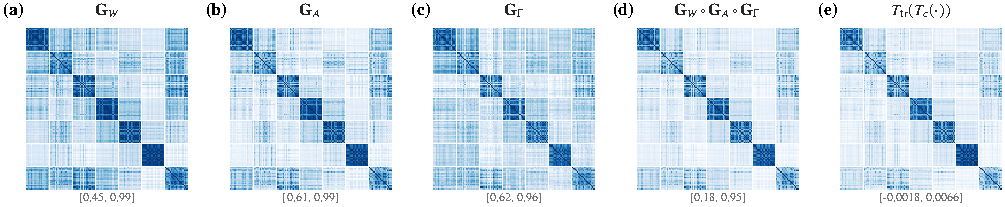
\includegraphics[width=\textwidth]{figuras/gram_construcao.pdf}
\caption{Construção da matriz de Gram, ilustrada sobre a base \texttt{segment} (sete classes, vinte amostras por classe), no bloco \texttt{b3} do perceptron multicamadas com alvo fixo. Da esquerda para a direita são apresentadas as matrizes de Gram componentes ($\mathbf{G}_W$, $\mathbf{G}_A$ e $\mathbf{G}_\Gamma$), o produto de Hadamard que as compõe e a matriz de Gram após o centramento e a normalização em traço. Os objetos estão ordenados por classe, com as fronteiras entre as classes marcadas por linhas claras, e tons escuros indicam maior similaridade.}
\label{fig:gram_construcao}
\end{figure}

\subsection{Experimentos}\label{subsec:experimentos}

Os experimentos são divididos em cinco famílias, de acordo com a referência que cada uma utiliza, além da datação por intervenção.

A \textbf{primeira família} (P1 e P2) reúne as leituras da matriz de distância: a acurácia de $k$-vizinhos \textit{leave-one-out} contra a predição do modelo, a área sob a curva ROC da margem geométrica como preditora do acerto e a correlação de Spearman, no nível de classe, entre a proximidade geométrica dos pares de classes e a \textbf{confusão suave}, isto é, a probabilidade média que o modelo atribui à classe $b$ nas amostras da classe $a$, simetrizada e calculada sobre o teste inteiro.

A \textbf{segunda família} (P4) reúne as leituras do espectro, obtidas da decomposição $\mathbf{G} = V\Lambda V^\top$: a fração das direções de classe contida em $V_r$ e a razão de energia ortogonal $\widehat{E}_{\mathrm{ratio}}$ como preditora do erro. Como essas leituras dependem de $r$, as comparações entre representações utilizam o mesmo $r = K-1$ para todas, para que uma diferença no número de modos retidos não seja lida como uma diferença de geometria.

A \textbf{terceira família} (P2 e P3) reúne as ablações e referências: cada fonte isolada, a análise representacional clássica (RSA) com distância euclidiana sobre as ativações e a decomposição contra a CKA, $\hat{\mathbf{G}} = a\,\hat{K}_{\mathrm{ativ}} + R$, com $a = \mathrm{CKA}(\mathbf{G}, K_{\mathrm{ativ}})$. Cada parte é projetada no cone semidefinido positivo, registrando-se a massa espectral descartada, e avaliada pelas leituras de comportamento.

A \textbf{quarta família} (P5) toma como objetos as posições espaciais de uma única imagem e reúne o campo de energia e os conjuntos de nível, validados pela máscara do animal e por deleção, conforme detalhado na Subseção \ref{subsec:res_campo}.

A \textbf{quinta família} (P6) é a leitura contrastiva e contrafactual do método. Para cada amostra $i$ classificada corretamente, toma-se como par a amostra $j$ mais próxima de $i$ nos atributos entre aquelas que o modelo classifica de outra forma. Pela definição da Seção \ref{sec:referencial}, $j$ é um contrafactual observado de $i$, o vizinho mais próximo de classe distinta \citep{KeaneSmyth2020}. A pergunta é quais das diferenças entre $i$ e $j$ importam para o modelo. Nos dados tabulares, cada atributo $f$ recebe a pontuação
\begin{equation}\label{eq:delta_d}
    \Delta d_f \;=\; d(i,j) - d(i^{(f)},j),
\end{equation}
em que $i^{(f)}$ é a amostra $i$ com o atributo $f$ levado ao valor de $j$, e $d$ é a distância da Gram conjunta com alvo fixo. Isto é, $\Delta d_f$ mede quanto a intervenção $do(x_f := x_{j,f})$ aproxima $i$ do seu contrafactual no espaço do modelo. Essa leitura exige apenas as $F + 2$ linhas formadas por $i$, $j$ e as $F$ versões de $i$ com um atributo trocado. A validação é externa à geometria e constrói contrafactuais sintéticos: trocam-se os $k$ primeiros atributos do ranking e mede-se se a predição de $i$ passa a ser a de $j$, como faz o algoritmo NICE \citep{Brughmans2024}. Um ranking melhor produz um contrafactual válido com menos trocas, isto é, mais próximo de $i$. Nas imagens, a unidade é a região, as posições das duas imagens entram em uma única matriz de Gram de ordem $2P$ e a validação é a deleção das regiões na ordem do mapa, medindo a margem $f_{c_i} - f_{c_j}$.

Por fim, a \textbf{datação} (P8) é obtida por intervenção sobre os estados internos. Em modo de inferência, a rede é um modelo causal estrutural determinístico e sem confundimento, em que $h_\ell = f_\ell(h_{\ell-1})$, de modo que a intervenção pode ser executada diretamente, em vez de estimada \citep{Pearl2009}:
\begin{equation}\label{eq:intervencao}
    R(\ell,\sigma) \;=\; \Pr\Bigl(\hat{y} \neq \hat{y}_{\text{limpo}}
    \;\Bigm|\; do\bigl(h_\ell := h_\ell + \sigma\,s_\ell \odot \varepsilon\bigr)\Bigr),
    \qquad \varepsilon \sim \mathcal{N}(0, I),
\end{equation}
em que $s_\ell$ é o vetor de desvios-padrão por canal do bloco, o que torna $\sigma$ um orçamento comparável entre blocos.

\subsection{Estudos de caso}\label{subsec:estudos_caso}

As famílias anteriores medem se as leituras se sustentam entre bases e sementes, mas comparam o método apenas com pisos e referências simples. Dois estudos de caso sobre a base \texttt{letter} \citep{FreySlate1991} complementam essa avaliação. A base foi escolhida porque os seus dezesseis atributos têm significado (posição e dimensões da caixa que envolve a letra, número de píxeis acesos, momentos e contagens de bordas), porque possui 26 classes e porque, com $F = 16$, o valor de Shapley de um par pode ser calculado de forma exata. Até onde sabemos, a base não havia sido objeto de um estudo de interpretabilidade.

\subsubsection*{O método, o SHAP, o LIME e uma árvore de decisão sobre o mesmo modelo}

O primeiro estudo responde a P6 e compara o método às duas técnicas de atribuição mais utilizadas, o SHAP \citep{LundbergLee2017} e o LIME \citep{Ribeiro2016}, ambas modelo-agnósticas. O modelo explicado é o perceptron multicamadas, com cinco sementes e cem pares contrafactuais por semente, escolhidos como na quinta família. O ranking do método é o da Gram conjunta de \texttt{b3}.

Cada técnica é avaliada em duas formas. A \textbf{forma contrastiva} explica a margem $m = f_{c_j} - f_{c_i}$ tomando $j$ como referência, e responde à mesma pergunta que o método. No SHAP, ela inclui o valor de Shapley exato do jogo $v(S) = m(x_j^{S}, x_i^{\bar S}) - m(x_i)$, isto é, o \textit{baseline Shapley} com $j$ de referência \citep{SundararajanNajmi2020}, e o SHAP intervencional usual lido como $\phi_m(x_j) - \phi_m(x_i)$. No LIME, o modelo linear local é ajustado sobre $m$ em torno de $x_i$, e cada atributo é pontuado pela variação prevista ao levá-lo ao valor de $j$. A \textbf{forma usual} explica apenas a amostra $i$, como as técnicas costumam ser aplicadas. O valor de Shapley exato é a decomposição da própria troca que o teste contrafactual mede e, por isso, funciona como o limite superior do teste. Como o método não amostra e tem custo fixo por par, as técnicas também são comparadas com o mesmo orçamento de avaliações do modelo, estimando o Shapley por permutações amostradas \citep{Strumbelj2014} e variando o número de perturbações do LIME.

A árvore de decisão \citep{Breiman1984} é treinada diretamente sobre os rótulos, sem acesso ao perceptron. Para um par $(i,j)$, a explicação da própria árvore é o atributo do nó em que os caminhos de $i$ e de $j$ se separam, e a leitura é a posição desse atributo em cada ranking, nos pares em que a árvore reproduz as duas predições do perceptron. A árvore é uma corroboração, e não uma verdade de referência: a concordância indica que dois modelos independentes se apoiam nos mesmos atributos. No nível global, as importâncias do método, do SHAP, do LIME e da árvore são comparadas com a importância por permutação no perceptron \citep{Breiman2001}.

\subsubsection*{O método aplicado a uma árvore de decisão}

O segundo estudo responde a P7 na sua forma mais forte. Se o método é modelo-agnóstico, aplicá-lo a um modelo sem ativações contínuas nem gradiente deve exigir apenas outra escolha de fontes. Além disso, a árvore explica a si mesma pelo seu caminho de decisão, o que fornece uma resposta conhecida.

Nesta instanciação, os blocos são as profundidades $\ell$ da árvore, e cada amostra possui três fontes em cada profundidade. A fonte de \textbf{caminho} é o indicador dos nós visitados até $\ell$, o estado da árvore. A fonte de \textbf{folga} registra, em cada nó já atravessado, a quantidade $(x_f - t)/\sigma_f$, isto é, quanto falta para a amostra mudar de ramo. A fonte de \textbf{classes} é a distribuição de classes do nó atual, o que a árvore decidiria naquele ponto. A composição e a leitura de pares são as mesmas das redes.

A árvore fornece três referências. A primeira é o atributo do nó de separação, que deve ser o primeiro do ranking. A segunda é a profundidade dessa separação, que deve coincidir com a profundidade em que esse atributo passa a ser o primeiro do método, verificando a datação de P8 contra uma resposta exata. A terceira é o contrafactual mínimo, isto é, o menor conjunto de trocas que muda a predição da árvore, obtido por enumeração dos $2^{16}$ subconjuntos. O piso é o método aplicado a uma árvore treinada sobre rótulos embaralhados.

\subsection{Referências de nulidade}\label{subsec:pisos}

Um piso indica o valor de uma leitura se a geometria não carregasse nenhuma informação, e apenas a geometria deve mudar entre a medida e o seu piso. Nas leituras referidas ao comportamento, medir o modelo não treinado contra a sua própria predição mudaria a geometria e o alvo ao mesmo tempo, e além disso é degenerado: na inicialização, a predição se concentra em uma única classe na maior parte da amostra, o que a torna trivial de recuperar. Por esse motivo é adotado o \textbf{piso cruzado}, em que a geometria do modelo não treinado é medida contra o comportamento do modelo treinado, de modo que a única diferença entre a medida e o piso é o treinamento.

Três pisos adicionais acompanham leituras específicas. Nas leituras espaciais, um mapa que marca apenas o centro da imagem, visto que o animal tende a ocupar o centro. Nas leituras de pares, um piso de especificidade, o mesmo mapa calculado contra uma terceira amostra de classe não envolvida, visto que um mapa que não o supera indica o que importa em $i$, e não o que distingue $i$ de $j$. Nas leituras de pares, também a ordem aleatória entre os atributos que diferem. Por fim, as comparações entre representações são estritas, de modo que empates não contam como vitória, e leituras indefinidas são excluídas da contagem, e não tratadas como falhas.

\subsection{Reprodutibilidade}\label{subsec:reprodutibilidade}

Todos os experimentos utilizam semente fixa na partição dos dados, na seleção da amostra, na inicialização e nas intervenções estocásticas. Cada execução grava um relatório com todas as medidas, os seus pisos e a configuração completa, de modo que qualquer tabela pode ser reconstruída sem repetir o treinamento. O método está disponível como a biblioteca \texttt{fannar}, que implementa o pipeline núcleo-transformação para matrizes de Gram arbitrárias, as leituras e as fontes das duas instanciações. Quanto ao custo, a análise do método está na Subseção \ref{subsec:custo}. A instanciação acrescenta a extração das fontes, uma passagem direta e uma reversa por objeto, isto é, $\Theta(nT)$ para um modelo cuja passagem direta custa $T$ \citep{GriewankWalther2008}, e a leitura de um par custa $\Theta\bigl(F\,T\bigr)$, contra $\Theta\bigl(2^F\,T\bigr)$ do valor de Shapley exato. O treinamento de cada modelo leva de poucos minutos a cerca de uma hora em uma única placa gráfica.

\section{Resultados}\label{sec:resultados}

Os resultados a seguir avaliam a instanciação descrita na Seção \ref{sec:metodologia}, e não o método em si, cujas propriedades (semidefinição positiva, pseudométrica e decomposição da energia espectral) foram demonstradas nas Seções \ref{sec:tensor_rkhs} a \ref{sec:representation_geometry}. Eles são apresentados na ordem das perguntas da Subseção \ref{subsec:perguntas}, e, salvo menção explícita, os valores são os da variante de \textbf{alvo fixo}. O motivo dessa convenção fica claro com um exemplo. Na ResNet, os $k$ vizinhos mais próximos de uma imagem na Gram conjunta de \texttt{b3} recuperam a predição do modelo em $95{,}6\%$ dos casos quando o gradiente é tomado em relação à classe predita, e em apenas $20{,}4\%$ com alvo fixo. A primeira leitura não é um acerto do método: o gradiente já carrega a predição, e reencontrá-la é como procurar uma resposta que foi escrita na pergunta.

\subsection{P1: A geometria reflete o comportamento do modelo?}\label{subsec:res_comportamento}

Se o espaço reflete o entendimento do modelo, os vizinhos de uma amostra devem ter a mesma predição que ela, as amostras que o modelo erra devem estar em regiões ambíguas e as classes que o modelo confunde devem estar próximas entre si. A Tabela \ref{tab:res_estabilidade} e a Figura \ref{fig:res_estabilidade} apresentam essas leituras para as dez bases tabulares.

\begin{table}[htbp]
\centering
\caption{Leituras de comportamento nas dez bases tabulares (cinquenta execuções, alvo fixo). Média entre bases, do \texttt{stem} a \texttt{b6}, o piso cruzado da Gram conjunta, que é plano na profundidade, e a fração das execuções em que a Gram conjunta supera estritamente esse piso. As leituras espectrais não se aplicam à análise representacional (RSA).}
\label{tab:res_estabilidade}
\footnotesize
\setlength{\tabcolsep}{4pt}
\begin{tabular}{l c c c c c}
\hline
Leitura & Conjunta & Ativações & RSA & Piso & Acima do piso \\
\hline
$k$-vizinhos contra a predição & $0{,}882 \to 0{,}975$ & $0{,}851 \to 0{,}974$ & $0{,}852 \to 0{,}974$ & $0{,}805$ & 100\% \\
AUC da margem para o acerto & $0{,}824 \to 0{,}965$ & $0{,}804 \to 0{,}961$ & $0{,}764 \to 0{,}940$ & $0{,}767$ & 81\% a 100\% \\
Confusão suave (Spearman) & $0{,}463 \to 0{,}400$ & $0{,}460 \to 0{,}447$ & $0{,}354 \to 0{,}342$ & $0{,}422$ & 44\% a 76\% \\
Contenção em $V_r$ ($r = K-1$) & $0{,}568 \to 0{,}831$ & $0{,}475 \to 0{,}826$ & & $0{,}416$ & 100\% \\
$\widehat{E}_{\mathrm{ratio}}$ para o erro & $0{,}658 \to 0{,}788$ & $0{,}635 \to 0{,}787$ & & $0{,}598$ & 84\% a 100\% \\
\hline
\end{tabular}
\end{table}

\begin{figure}[htbp]
    \centering
    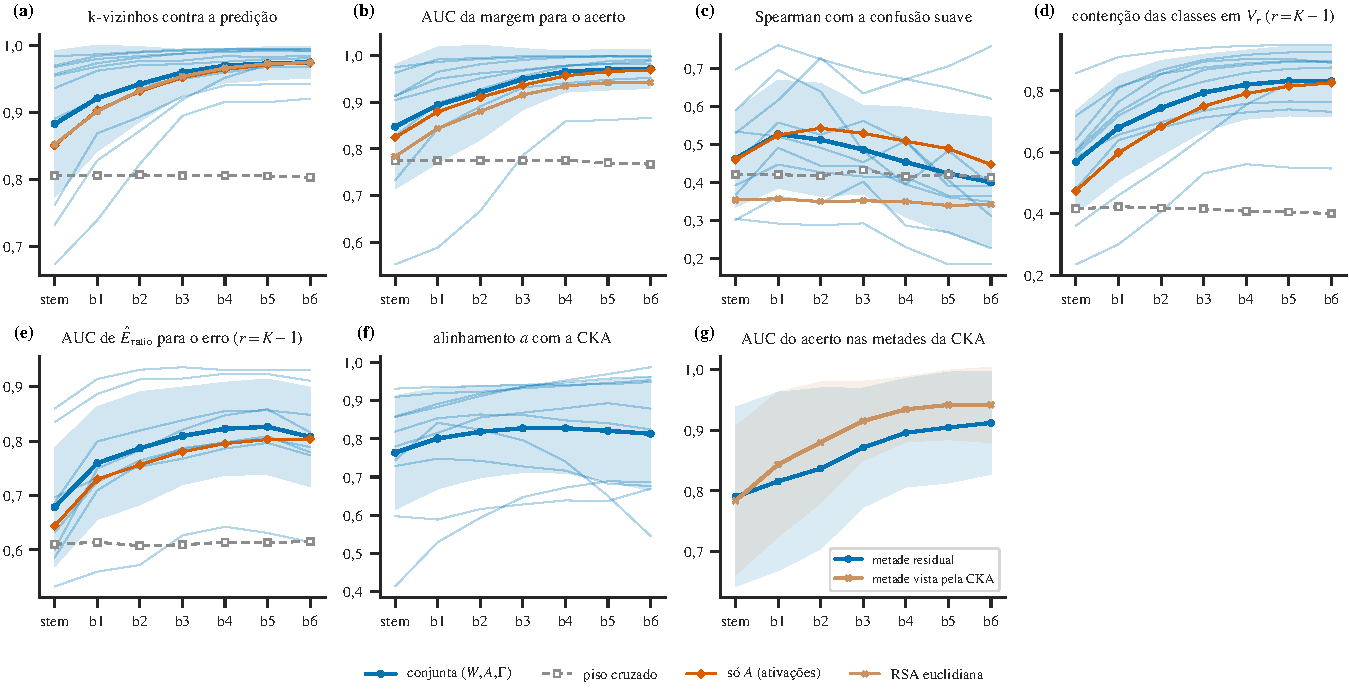
\includegraphics[width=\textwidth]{figuras/res_estabilidade.pdf}
    \caption{Leituras por bloco nas dez bases tabulares, com alvo fixo. A linha grossa é a média entre bases da Gram conjunta, as linhas finas são as bases isoladas e a faixa é o desvio entre bases. A linha tracejada é o piso cruzado, e as demais séries são a fonte de ativações isolada e a análise representacional euclidiana. (a) Recuperação da predição por $k$-vizinhos. (b) Área sob a curva ROC da margem geométrica para o acerto. (c) Concordância com a confusão suave. (d) Contenção das direções de classe em $V_r$. (e) $\widehat{E}_{\mathrm{ratio}}$ como preditor do erro. (f) Alinhamento com a Gram das ativações. (g) Acerto previsto pelas duas partes da decomposição contra a CKA.}
    \label{fig:res_estabilidade}
\end{figure}

A recuperação da predição por $k$-vizinhos fica acima do piso em todas as execuções e em todos os blocos (Figura \ref{fig:res_estabilidade}a). O piso, entretanto, é alto ($0{,}805$), e isso é uma propriedade dos dados: as classes dessas bases já são quase separáveis nos atributos brutos, e um modelo na inicialização preserva boa parte dessa estrutura. Por esse motivo, o Oxford-IIIT Pet funciona como contraprova. Com 37 raças, o piso cai para cerca de $0{,}06$, e a Gram conjunta da ResNet cresce de $0{,}069$ no \texttt{stem} para $0{,}603$ em \texttt{b6}, acima do piso em todas as sementes a partir de \texttt{b1} (Figura \ref{fig:res_pets}a).

A segunda leitura é a mais diretamente útil. A margem geométrica de uma amostra, isto é, o quanto ela está mais próxima de amostras com a sua própria predição do que de amostras com outras predições, prevê se o modelo a acerta, acima do piso nas bases tabulares e em todas as sementes e blocos do Pet (Figuras \ref{fig:res_estabilidade}b e \ref{fig:res_pets}b). A intuição é a mesma do \textit{trust score} \citep{Jiang2018} e dos $k$-vizinhos profundos \citep{Papernot2018}: uma predição cercada de vizinhos classificados de outra forma merece menos confiança. Na prática, essa leitura permite encaminhar as predições menos plausíveis de um modelo implantado para revisão humana. Ela ainda não foi comparada à confiança do próprio \textit{softmax} \citep{Hendrycks2017}.

A terceira leitura, a concordância com a confusão, separa as duas famílias de dados. Nas bases tabulares, ela não se sustenta nos blocos profundos, ficando acima do piso em apenas 44\% a 47\% das execuções em \texttt{b5} e \texttt{b6} (Figura \ref{fig:res_estabilidade}c). No Pet, ela cresce de $0{,}170$ para $0{,}674$, contra um piso em torno de $0{,}21$, e supera o piso em todas as sementes a partir de \texttt{b1} (Figura \ref{fig:res_pets}c). A diferença é simples: nas bases tabulares o modelo quase não erra, e a confusão entre a maior parte dos pares de classes é praticamente nula. No Pet, raças confundíveis produzem uma estrutura de confusão rica, e a geometria a reproduz.

\begin{figure}[htbp]
    \centering
    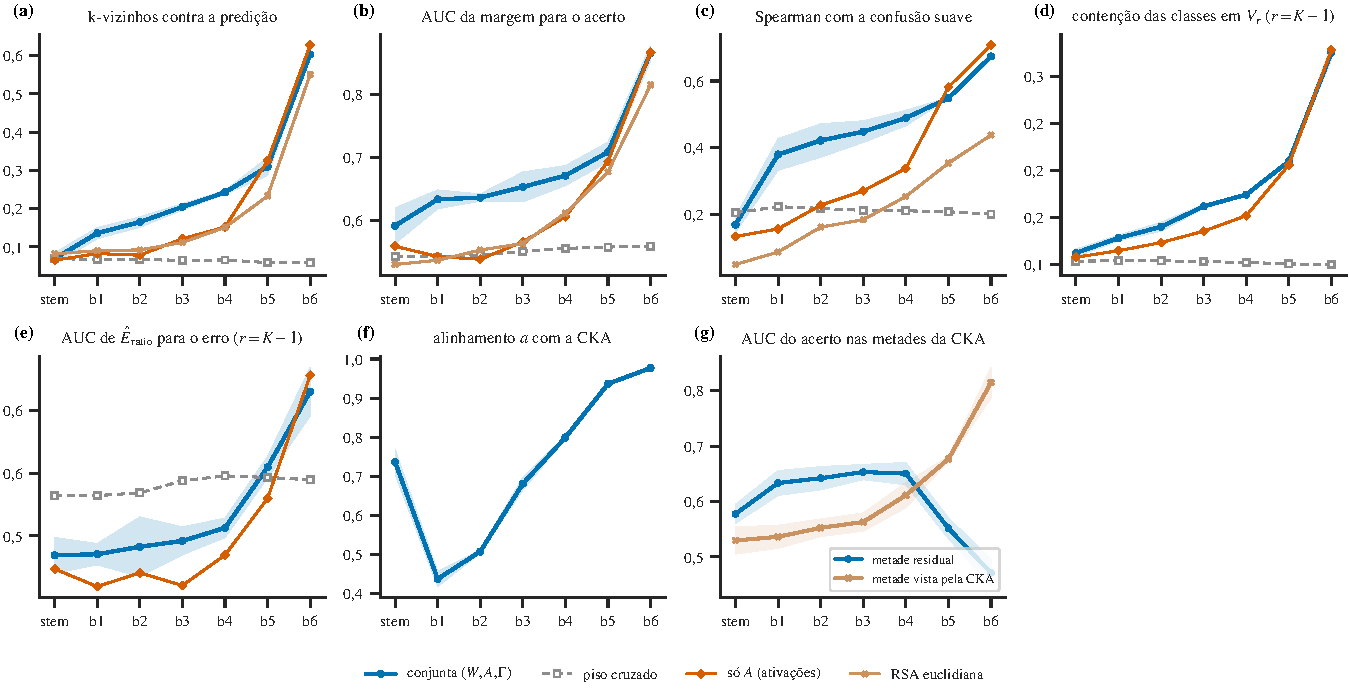
\includegraphics[width=\textwidth]{figuras/res_pets.pdf}
    \caption{As mesmas leituras da Figura \ref{fig:res_estabilidade} no Oxford-IIIT Pet, com a ResNet (três sementes, alvo fixo). A faixa é o desvio entre sementes. Diferentemente das bases tabulares, o piso do $k$-vizinhos fica próximo do acaso ($1/37$), e a concordância com a confusão supera o piso a partir de \texttt{b1}.}
    \label{fig:res_pets}
\end{figure}

A resposta a P1 é, portanto, afirmativa para a decisão e para o erro, e condicionada para a confusão, que só se sustenta quando o modelo confunde classes de forma estruturada.

\subsection{P2: A composição acrescenta algo às fontes isoladas?}\label{subsec:res_composicao}

A resposta depende de onde a leitura é feita. Nas bases tabulares, a Gram conjunta supera a fonte de ativações na recuperação da predição em 90\% das execuções no \texttt{stem}, mas essa vantagem decresce até 32\% em \texttt{b6}. No Pet, o padrão é o mesmo e mais nítido: a conjunta supera as ativações em todas as sementes de \texttt{b1} a \texttt{b4}, nas três leituras de comportamento, e a vantagem desaparece nos dois últimos blocos (Figura \ref{fig:res_pets}). Contra a RSA, a composição vence na previsão do acerto em 84\% a 91\% das execuções tabulares e em todas as sementes e blocos da ResNet.

A origem da vantagem é o gradiente contrastivo. Nos blocos rasos, as ativações descrevem o conteúdo local da imagem (bordas, texturas e cores), e duas imagens de raças diferentes com o mesmo fundo parecem semelhantes para $A$. O gradiente, por outro lado, descreve como a decisão responderia a uma mudança naquele estado, e já é específico da classificação. De fato, na ResNet, $\Gamma$ isolado praticamente iguala a composição de \texttt{b1} a \texttt{b4}. Nos blocos profundos, as ativações já carregam a decisão, e a composição deixa de acrescentar.

\subsection{P3: O método se distingue de uma simples CKA?}\label{subsec:res_cka}

A decomposição $\hat{\mathbf{G}} = a\,\hat{K}_{\mathrm{ativ}} + R$ responde a essa pergunta em termos de conteúdo. Um resultado torna a decomposição fácil de interpretar: a parte vista pela CKA, $a\,\hat{K}_{\mathrm{ativ}}$, produz exatamente os mesmos valores que a RSA euclidiana em todas as leituras, sementes e arquiteturas. Isso não é coincidência, visto que as distâncias induzidas pela Gram linear centrada das ativações são as distâncias euclidianas entre elas. A parte que a CKA enxerga é, portanto, a geometria euclidiana das ativações, e o resíduo $R$ é tudo aquilo que uma análise das ativações não enxerga.

Nas bases tabulares, o alinhamento $a$ fica entre $0{,}76$ e $0{,}83$, e o resíduo prevê o acerto pior do que a parte vista em cerca de três quartos das execuções (Figura \ref{fig:res_estabilidade}g), o que favorece a CKA. Na ResNet, o resultado se inverte nos blocos rasos e intermediários: o alinhamento cai para $0{,}44$ em \texttt{b1}, e o resíduo prevê o acerto melhor do que a parte vista em todas as sementes do \texttt{stem} a \texttt{b4}, invertendo-se nos dois últimos blocos, onde o alinhamento sobe para $0{,}94$ e $0{,}98$ (Figura \ref{fig:res_pets}, painéis f e g). A resposta a P3 é, portanto, condicionada da mesma forma que P2: o método vê algo além da CKA onde as ativações ainda não carregam a decisão. Esse resultado é coerente com as limitações da CKA apontadas pela literatura, que mostram que ela é dominada pelos modos de maior variância das ativações \citep{Davari2023, Klabunde2025}.

\subsection{P4: A energia espectral descreve como o modelo representa cada amostra?}\label{subsec:res_espectro}

As leituras espectrais decompõem a Gram em modos e perguntam quais direções concentram a estrutura do espaço e quanto de cada amostra vive fora delas. A primeira afirmação, de que as direções de classe estão contidas em $V_r$, é a mais robusta da instanciação. Com $r = K-1$, ela supera o piso em todas as execuções tabulares e em todos os blocos, e a Gram conjunta supera as ativações em 88\% a 100\% das execuções em toda a profundidade (Figura \ref{fig:res_estabilidade}d). No Pet, os valores são menores, de $0{,}112$ para $0{,}325$, mas ficam acima do piso de $0{,}10$ a partir de \texttt{b1} (Figura \ref{fig:res_pets}d). Isto é, as poucas direções dominantes do espaço construído são as direções em que o modelo separa as suas decisões, e a composição concentra essa separação em menos modos do que as ativações.

A segunda afirmação depende da base. Nas bases tabulares, $\widehat{E}_{\mathrm{ratio}}$ prevê o erro acima do piso em 84\% a 100\% das execuções (Figura \ref{fig:res_estabilidade}e). Na ResNet, por outro lado, ela fica abaixo do piso do \texttt{stem} a \texttt{b4} e só o supera nos dois últimos blocos (Figura \ref{fig:res_pets}e). A ideia é a mesma da detecção de amostras fora da distribuição pelo resíduo do subespaço principal \citep{Wang2022ViM}, e o resultado mostra que esse indício só é confiável onde $V_r$ já é o subespaço da decisão. A razão de energia ortogonal é, portanto, a leitura menos robusta da instanciação.

\subsection{P5: O campo de energia e os conjuntos de nível apontam o que o modelo utiliza na entrada?}\label{subsec:res_campo}

Esta subseção toma como objetos as posições espaciais de uma única imagem, conforme o Comentário \ref{rem:diagnostic}. Em cada bloco, a posição $s$ carrega as três fontes, e as matrizes de Gram de ordem $P = HW$ são compostas pelo produto de Hadamard sem a normalização angular, que fixaria a energia de todas as posições. O campo de energia é a energia retida $\widehat{E}_{s,\parallel}$ da Equação \eqref{eq:empirical_energies}, calculada sobre 111 imagens de teste. A utilidade dessa leitura é auditar \textit{onde} o modelo olha, visto que um modelo pode acertar apoiando-se no fundo ou em um artefato da coleta \citep{Geirhos2020}.

\begin{figure}[htbp]
    \centering
    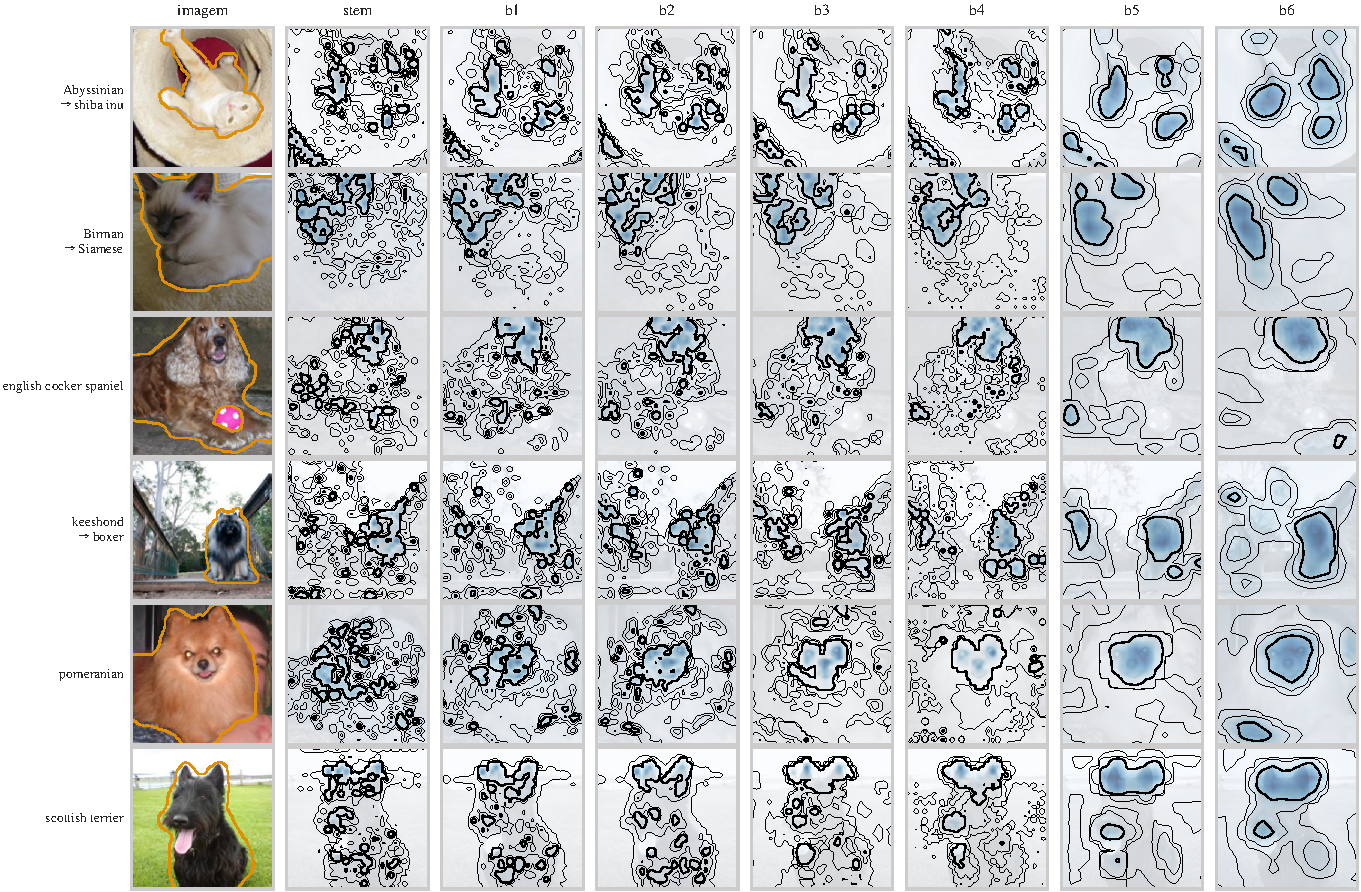
\includegraphics[width=\textwidth]{figuras/res_campo_resnet.pdf}
    \caption{Campo de energia da Gram conjunta da ResNet sobre seis imagens de teste do Oxford-IIIT Pet, do \texttt{stem} a \texttt{b6}. O contorno laranja na primeira coluna é a máscara do animal, utilizada apenas na avaliação, e os rótulos indicam a raça verdadeira e, quando o modelo erra, a predita. Tons escuros indicam maior energia retida.}
    \label{fig:res_campo_resnet}
\end{figure}

A primeira parte da pergunta é respondida afirmativamente. Na ResNet, o campo concentra de $0{,}82$ a $0{,}90$ da sua energia sobre o animal, contra $0{,}50$ de acaso, $0{,}66$ de um mapa que marca apenas o centro, $0{,}53$ a $0{,}78$ do Grad-CAM \citep{Selvaraju2017} e $0{,}47$ a $0{,}49$ da rede não treinada. Nos blocos rasos, o campo se espalha sobre o contorno e a textura do animal, e nos profundos se concentra em poucas regiões, tipicamente a cabeça (Figura \ref{fig:res_campo_resnet}). O campo também passa na verificação por aleatorização dos pesos \citep{Adebayo2018}, com correlação entre os campos da rede treinada e da não treinada próxima de zero.

A segunda parte não se sustenta com a mesma força. No teste de deleção \citep{Samek2017, Tomsett2020}, a Gram conjunta obtém de $0{,}47$ a $0{,}54$, contra $0{,}37$ do centro, e o Grad-CAM, calculado sobre o mesmo estado e o mesmo gradiente, a supera a partir de \texttt{b4}. Isto é, localizar o objeto e identificar a evidência da decisão são tarefas diferentes: um mapa pode cobrir todo o animal e, ainda assim, ordenar mal as suas partes \citep{Hooker2019, Nauta2023}.

\begin{figure}[htbp]
    \centering
    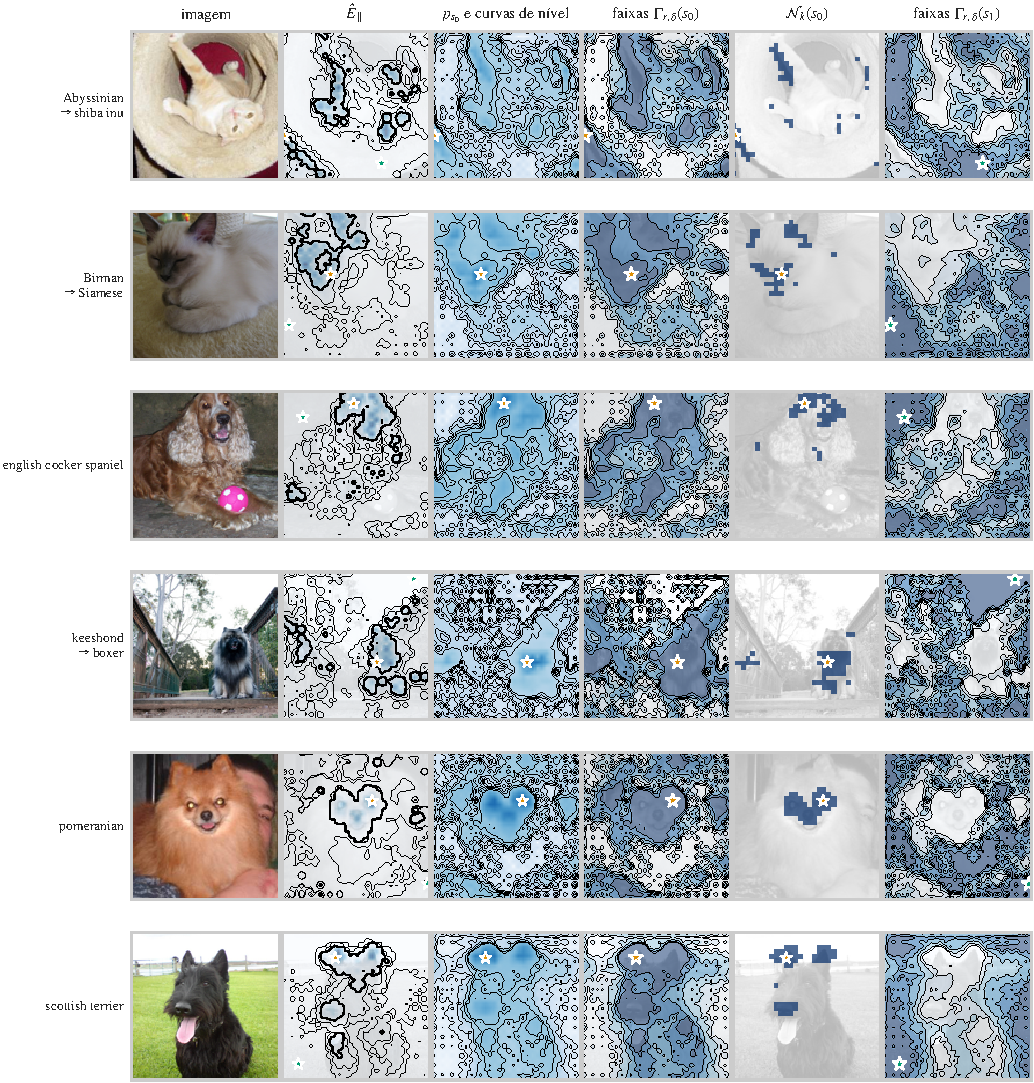
\includegraphics[width=\textwidth]{figuras/res_niveis.pdf}
    \caption{Conjuntos de nível no bloco \texttt{b4} da ResNet. Da esquerda para a direita, a figura mostra a imagem, o campo de energia com a referência $s_0$ (estrela laranja, medoide das posições de maior energia) e $s_1$ (estrela verde, medoide da metade de menor energia), a função distância $p_{s_0}$ com as suas curvas de nível, as faixas de nível $\Gamma_{r,\delta}(s_0)$, a vizinhança $\mathcal{N}_k(s_0)$ e as faixas em torno de $s_1$. No primeiro exemplo, $s_0$ cai na borda da imagem, sobre a faixa de energia alta produzida pelo preenchimento com zeros das convoluções.}
    \label{fig:res_niveis}
\end{figure}

Os conjuntos de nível da Equação \eqref{eq:sample_level_band} respondem à terceira parte: a partir de uma posição de referência $s_0$, quais regiões o modelo representa de forma semelhante? Para que a distância meça padrão, e não intensidade, a matriz do campo recebe a transformação angular $T_a$, e $s_0$ é o medoide das posições de maior energia. Com essa construção, a vizinhança de $s_0$ cai sobre o animal em $0{,}66$ no \texttt{stem} e em $0{,}90$ a $0{,}93$ nos blocos profundos, contra $0{,}44$ a $0{,}49$ da rede não treinada. A Figura \ref{fig:res_niveis} mostra o que essa leitura acrescenta ao campo: a vizinhança de $s_0$ reúne as regiões da cabeça, e não o corpo inteiro, isto é, separa as partes do animal que o modelo representa da mesma forma. Apagar as regiões na ordem da distância a $s_0$ remove a margem do modelo com diferença de áreas de $0{,}57$ a $0{,}59$ em \texttt{b4} e \texttt{b5}, contra no máximo $0{,}17$ da rede não treinada. Como mostra o primeiro exemplo da figura, a seleção de $s_0$ deve excluir a borda da imagem.

\subsection{P6: Por que esta amostra foi classificada de forma diferente daquela?}\label{subsec:res_diferencas}

Esta é a forma local do método e a mais próxima da maneira como as pessoas pedem explicações, que é contrastiva: não se pergunta por que algo aconteceu, e sim por que aconteceu isto em vez daquilo \citep{Miller2019}. Para cada amostra $i$, o par $j$ é o seu contrafactual observado mais próximo, e o método ordena as diferenças entre as duas pela pontuação $\Delta d_f$ da Equação \eqref{eq:delta_d}. A validação constrói contrafactuais sintéticos: se os primeiros atributos do ranking forem de fato os que distinguem as duas amostras para o modelo, levá-los ao valor de $j$ deve mudar a predição de $i$ para a de $j$ com poucas trocas.

\subsubsection*{Nas dez bases tabulares}

Sobre as dez bases e três sementes, com cinquenta pares por execução, a área sob a curva de trocas do método em \texttt{b3} é de $0{,}810$, contra $0{,}384$ da ordem aleatória e $0{,}607$ da rede não treinada, e o método supera essas duas referências em todas as execuções (Figura \ref{fig:res_diferencas}). Ele vence a atribuição de primeira ordem $\nabla f \cdot \Delta x$ em 87\% das execuções, mas empata com a diferença bruta $|\Delta x|$ ($0{,}812$), vencendo em 57\%. A área do método cresce com a profundidade do bloco, enquanto a da rede não treinada permanece plana, o que é coerente com P2: quanto mais a representação organiza a decisão, mais a distância nela aponta o que decide.

\begin{figure}[htbp]
    \centering
    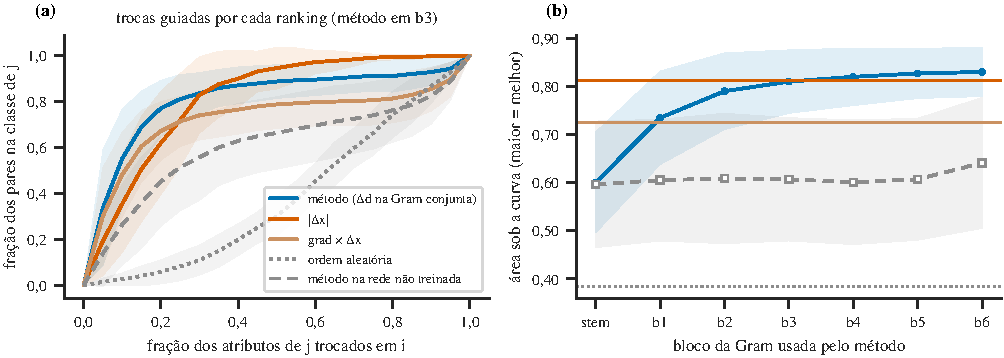
\includegraphics[width=\textwidth]{figuras/res_diferencas.pdf}
    \caption{Diferenças entre amostras nas dez bases tabulares. (a) Fração dos pares em que a amostra $i$ passa a ser classificada como $j$ conforme os $k$ primeiros atributos de cada ranking são trocados. (b) Área sob essa curva em função do bloco cuja Gram conjunta define o ranking, com as referências e o piso da rede não treinada.}
    \label{fig:res_diferencas}
\end{figure}

\subsubsection*{Estudo de caso: o método, o SHAP, o LIME e uma árvore de decisão}

Na \texttt{letter}, o perceptron atinge acurácia de $0{,}973 \pm 0{,}002$, e cada amostra difere do seu contrafactual, em média, em $9{,}4$ dos 16 atributos. A Tabela \ref{tab:res_letter} e a Figura \ref{fig:res_letter} reúnem os resultados sobre quinhentos pares.

\begin{table}[htbp]
\centering
\caption{Estudo de caso na \texttt{letter} (cinco sementes, cem pares por semente). Teste contrafactual de trocas (área sob a curva) e posição, em cada ranking, do atributo em que uma árvore de decisão treinada sobre os rótulos separa $i$ de $j$, nos pares em que ela reproduz as duas predições do perceptron (cerca de 71 por semente).}
\label{tab:res_letter}
\small
\begin{tabular}{l c c c}
\hline
Ranking & Área de trocas & Corte da árvore em 1º & Entre os 3 primeiros \\
\hline
Shapley exato com $j$ de referência & $0{,}862$ & $0{,}447$ & $0{,}737$ \\
\textbf{Método} (Gram conjunta, \texttt{b3}) & $\mathbf{0{,}803}$ & $\mathbf{0{,}416}$ & $\mathbf{0{,}691}$ \\
SHAP, $\phi(x_j) - \phi(x_i)$ & $0{,}775$ & $0{,}317$ & $0{,}657$ \\
LIME contrastivo, margem $f_{c_j} - f_{c_i}$ & $0{,}774$ & $0{,}388$ & $0{,}678$ \\
$|\Delta x|$ & $0{,}766$ & $0{,}262$ & $0{,}598$ \\
$\nabla f \cdot \Delta x$ & $0{,}711$ & $0{,}363$ & $0{,}572$ \\
SHAP só da amostra $i$ & $0{,}652$ & $0{,}233$ & $0{,}495$ \\
LIME só da amostra $i$ & $0{,}565$ & $0{,}218$ & $0{,}412$ \\
Método na rede não treinada & $0{,}651$ & $0{,}254$ & $0{,}510$ \\
Aleatória entre os que diferem & $0{,}639$ & $0{,}090$ & $0{,}316$ \\
\hline
\end{tabular}
\end{table}

\begin{figure}[htbp]
    \centering
    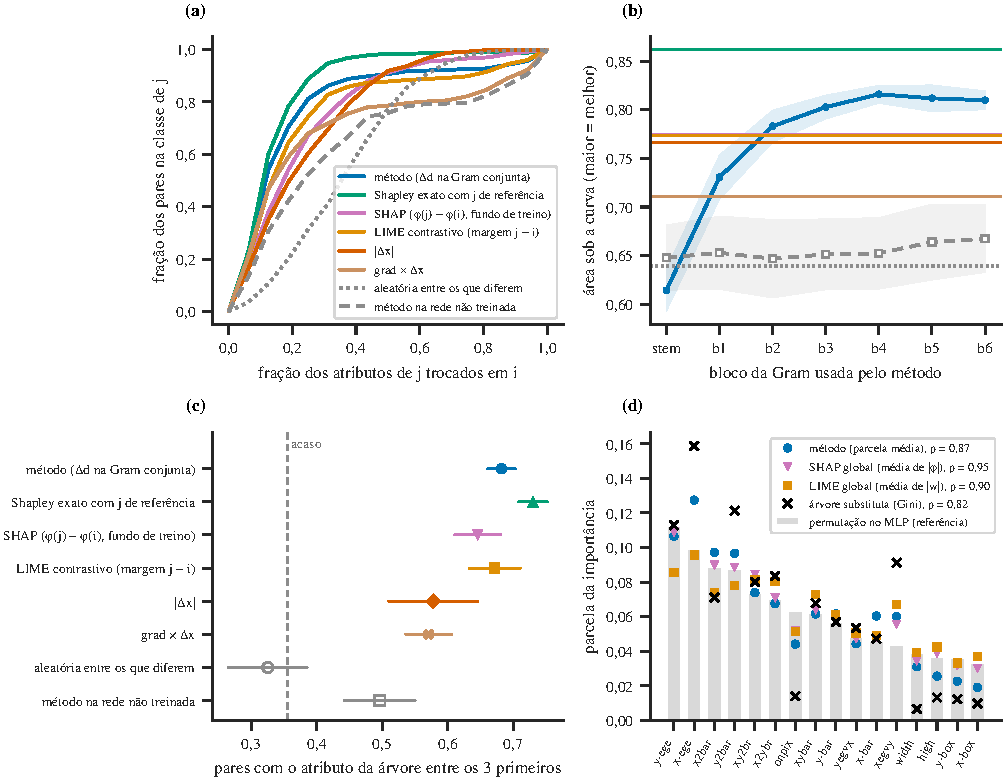
\includegraphics[width=\textwidth]{figuras/res_letter.pdf}
    \caption{Estudo de caso na \texttt{letter}. (a) Curvas de trocas de cada ranking, com o método em \texttt{b3}. (b) Área sob a curva do método em função do bloco, com as referências como linhas horizontais (mesmas cores e estilos de (a)). (c) Fração dos pares em que o atributo de separação da árvore de decisão está entre os três primeiros de cada ranking. (d) Importância global normalizada de cada atributo, na ordem da importância por permutação no perceptron (barras), e a correlação de Spearman de cada fonte com ela.}
    \label{fig:res_letter}
\end{figure}

Três resultados se destacam. O primeiro é que o método supera, em todas as sementes, o SHAP e o LIME nas formas contrastivas ($0{,}803$ contra $0{,}775$ e $0{,}774$) e, com mais folga, nas formas usuais, que explicam apenas a amostra $i$ ($0{,}652$ e $0{,}565$, este último abaixo até da ordem aleatória). A queda é instrutiva: as formas usuais explicam $i$ em relação a uma referência genérica, uma média do treino no SHAP e uma vizinhança amostrada no LIME, e não em relação ao contrafactual $j$. Uma explicação que não é contrastiva não responde à pergunta contrastiva.

O segundo resultado é que o método perde para o valor de Shapley exato com $j$ de referência ($0{,}862$). Isso é esperado, visto que esse jogo é a decomposição exata da própria troca que o teste mede \citep{SundararajanNajmi2020}. Os dois rankings concordam bastante, com correlação de Spearman mediana de $0{,}80$ e o mesmo atributo principal em 78\% dos pares. Uma comparação justa, entretanto, precisa considerar o custo. O método não amostra: ele sempre avalia as $F + 2 = 18$ linhas do par, o que equivale a cerca de 54 avaliações diretas do modelo, enquanto o SHAP e o LIME melhoram com mais avaliações. A Figura \ref{fig:res_orcamento} compara as técnicas com o mesmo orçamento.

\begin{figure}[htbp]
    \centering
    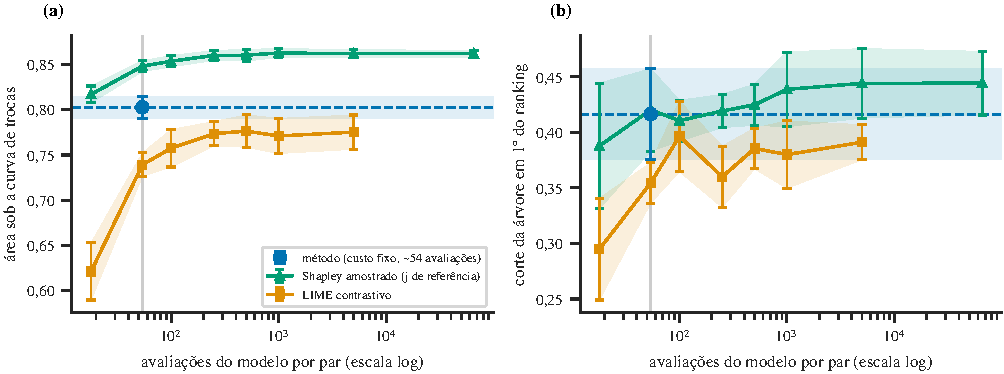
\includegraphics[width=\textwidth]{figuras/res_orcamento.pdf}
    \caption{Comparação com o mesmo orçamento de avaliações do modelo por par, na \texttt{letter} (cinco sementes, cem pares por semente). (a) Área sob a curva de trocas. (b) Fração dos pares em que o atributo de separação da árvore de decisão é o primeiro do ranking. As curvas são o valor de Shapley com $j$ de referência, estimado por permutações amostradas (o último ponto é o valor exato, com $2^{16}$ avaliações), e o LIME contrastivo. O método, que tem custo fixo, é o ponto sobre a linha vertical (cerca de 54 avaliações diretas) e a faixa horizontal. Pontos, barras e faixas indicam a média e o desvio padrão entre as sementes.}
    \label{fig:res_orcamento}
\end{figure}

O resultado divide as duas técnicas. O LIME contrastivo não alcança o método em nenhum orçamento, obtendo $0{,}739 \pm 0{,}013$ com as mesmas 54 avaliações e $0{,}775 \pm 0{,}019$ com cinco mil (Figura \ref{fig:res_orcamento}a). O valor de Shapley com $j$ de referência, ao contrário, supera o método com o mesmo custo, obtendo $0{,}848 \pm 0{,}006$ com três permutações. A explicação é que uma permutação desse jogo é, literalmente, levar os atributos de $i$ ao valor do contrafactual em uma ordem aleatória e registrar a variação da margem, isto é, o próprio teste. Na corroboração pela árvore, entretanto, as duas técnicas empatam com o mesmo custo (Figura \ref{fig:res_orcamento}b). A vantagem do método, portanto, não está no teste de trocas em si, e sim em que a mesma geometria responde também às perguntas P1 a P5, fornece a leitura por bloco e, como mostra a Subseção \ref{subsec:res_arquitetura}, recupera a explicação de uma árvore de decisão melhor do que o próprio Shapley exato.

O terceiro resultado é a corroboração por um modelo independente. A árvore de decisão treinada sobre os rótulos atinge acurácia de $0{,}850$ e concorda com o perceptron em 85\% das amostras de teste. Nos pares em que ela reproduz as duas predições, o atributo em que ela separa $i$ de $j$ está entre os três primeiros do método em 69\% dos pares, contra 68\% do LIME contrastivo, 66\% do SHAP e 36\% do acaso (Figura \ref{fig:res_letter}c). Isto é, dois modelos de natureza diferente apoiam-se nos mesmos atributos para distinguir as mesmas amostras, e o método recupera esse acordo a partir da geometria interna da rede. A árvore, entretanto, precisa de cerca de 1\,200 folhas e profundidade 27 para alcançar essa acurácia, o que a torna pouco legível e reforça o argumento de explicar o modelo que se usa, e não um substituto mais simples \citep{Rudin2019}.

Por fim, o método mostra em que profundidade da rede cada atributo passa a importar, algo que o SHAP e o LIME não separam. Em um par em que o perceptron classifica uma letra como G e outra como E, a dispersão horizontal dos píxeis acesos (\texttt{x2bar}) responde por 0\% da aproximação no \texttt{stem}, por 36\% em \texttt{b3} e novamente por 0\% em \texttt{b6}, isto é, essa distinção é usada no meio da rede e depois absorvida. No nível global, por outro lado, o SHAP ($0{,}95$) e o LIME ($0{,}90$) concordam mais com a importância por permutação do que o método ($0{,}87$) e a árvore ($0{,}82$) (Figura \ref{fig:res_letter}d).

\subsubsection*{Nas imagens}

Nas imagens, a leitura usa a Gram cruzada de duas imagens. Sobre vinte pares do Pet, entre raças que o modelo confunde ou da mesma raça com uma classificação correta e outra errada, o mapa do método derruba a margem $f_{c_i} - f_{c_j}$ mais do que a rede não treinada e a ordem aleatória, mas não supera o mapa de centro e falha no piso de especificidade: o mesmo mapa calculado contra uma terceira imagem, de raça não envolvida, derruba a margem quase tanto. O Grad-CAM contrastivo, calculado sobre o gradiente da mesma margem, supera o método a partir de \texttt{b4}. Sendo assim, nas imagens, o mapa indica quais regiões sustentam a decisão de $i$, e não quais a distinguem do contrafactual $j$.

\subsection{P7: As leituras dependem do modelo?}\label{subsec:res_arquitetura}

Esta pergunta é respondida em dois níveis: o mesmo código aplicado a um transformador de visão e o método aplicado a um modelo que não é uma rede neural, a árvore de decisão da \texttt{letter}.

\subsubsection*{O transformador de visão}

\begin{table}[htbp]
\centering
\caption{Leituras por imagem no Oxford-IIIT Pet para as duas arquiteturas (três sementes cada, alvo fixo), do \texttt{stem} a \texttt{b6}, e o piso cruzado de cada uma. Todas as leituras superam o piso em todas as sementes a partir de \texttt{b1}, exceto $\widehat{E}_{\mathrm{ratio}}$ nos blocos rasos da ResNet.}
\label{tab:res_arquitetura}
\small
\begin{tabular}{l c c c c}
\hline
 & \multicolumn{2}{c}{ResNet} & \multicolumn{2}{c}{Transformador} \\
Leitura & Conjunta & Piso & Conjunta & Piso \\
\hline
$k$-vizinhos contra a predição & $0{,}069 \to 0{,}603$ & $0{,}06$ & $0{,}132 \to 0{,}559$ & $0{,}04$ a $0{,}07$ \\
AUC da margem para o acerto & $0{,}591 \to 0{,}865$ & $0{,}54$ a $0{,}56$ & $0{,}629 \to 0{,}823$ & $0{,}51$ a $0{,}52$ \\
Confusão suave (Spearman) & $0{,}170 \to 0{,}674$ & $0{,}21$ & $0{,}495 \to 0{,}738$ & $0{,}09$ a $0{,}24$ \\
Contenção em $V_r$ ($r = K-1$) & $0{,}112 \to 0{,}325$ & $0{,}10$ & $0{,}139 \to 0{,}240$ & $0{,}10$ \\
$\widehat{E}_{\mathrm{ratio}}$ para o erro & $0{,}485 \to 0{,}615$ & $0{,}53$ a $0{,}55$ & $0{,}507 \to 0{,}663$ & $0{,}52$ a $0{,}54$ \\
\hline
\end{tabular}
\end{table}

As leituras por imagem se transferem ao transformador sem nenhuma alteração do código (Tabela \ref{tab:res_arquitetura}), e a razão de energia ortogonal, que falhava nos blocos rasos da ResNet, supera o piso em todas as sementes de \texttt{b1} a \texttt{b6}. O que muda é a origem da informação. No transformador, o gradiente contrastivo isolado quase não carrega informação sobre o comportamento, e a composição só supera as ativações de forma consistente no \texttt{stem}, de modo que a decomposição contra a CKA favorece a CKA a partir de \texttt{b2}. A contenção em $V_r$, por outro lado, continua favorecendo a composição em todos os blocos. Sendo assim, a forma do método independe da arquitetura, mas a contribuição de cada fonte não: o que o gradiente acrescenta às ativações é uma propriedade da rede convolucional, e não do método.

\begin{figure}[htbp]
    \centering
    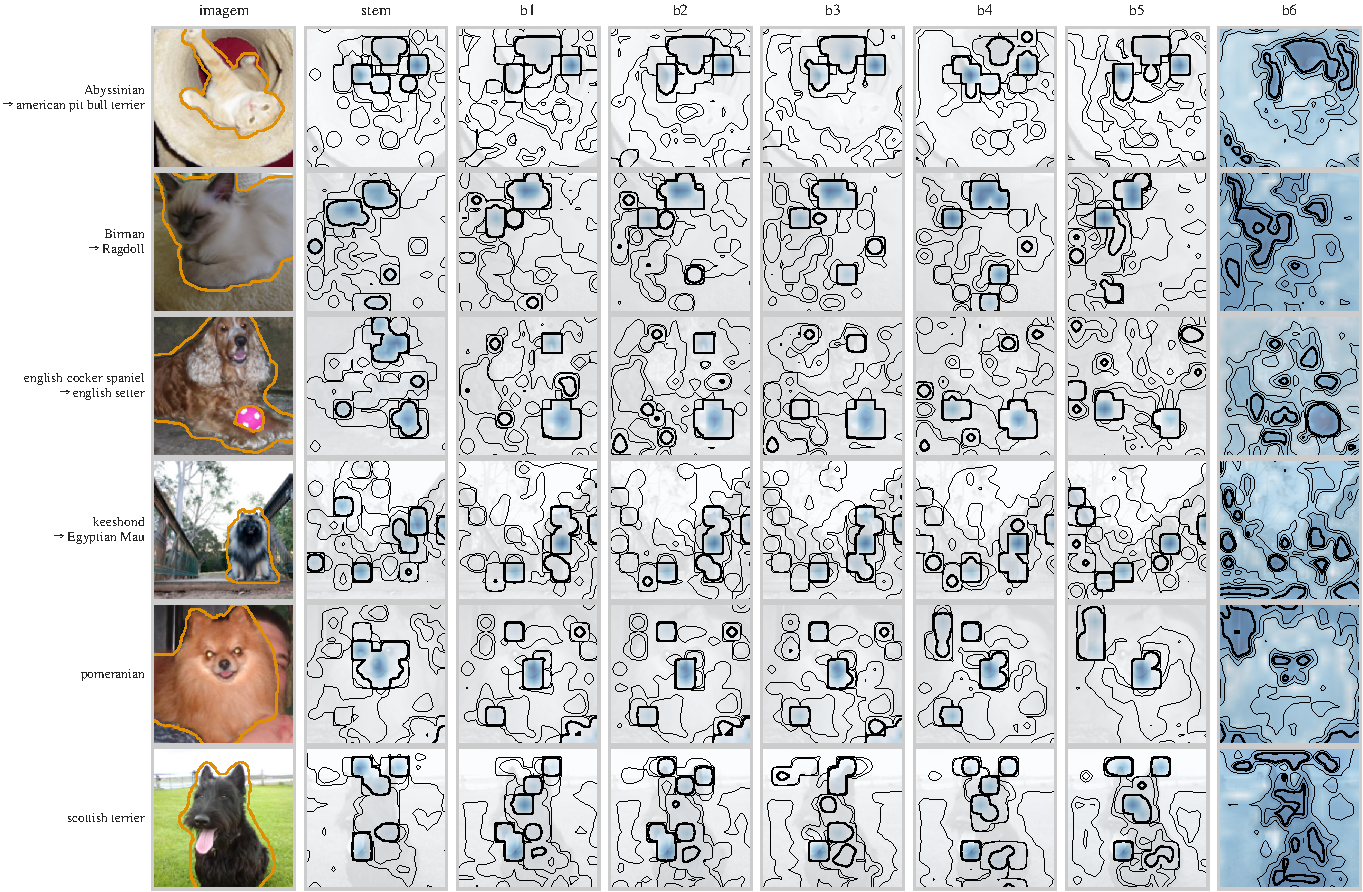
\includegraphics[width=\textwidth]{figuras/res_campo_vit.pdf}
    \caption{Campo de energia da Gram conjunta do transformador sobre as mesmas imagens da Figura \ref{fig:res_campo_resnet}. O aspecto quadriculado vem da grade de \textit{tokens} ($16 \times 16$), ampliada para a imagem. No último bloco, a cabeça é um \textit{pooling} médio seguido de uma camada linear, de modo que o gradiente é o mesmo em todas as posições e o campo deixa de distinguir regiões.}
    \label{fig:res_campo_vit}
\end{figure}

As leituras sobre a entrada, entretanto, não se transferem. No transformador, a fração da energia sobre o animal cai de $0{,}83$ no \texttt{stem} para perto do piso de centro nos blocos seguintes, e o teste de deleção fica abaixo do centro em todos os blocos (Figura \ref{fig:res_campo_vit}). A explicação mais provável é estrutural: a atenção mistura informação de toda a imagem já nas primeiras camadas \citep{Raghu2021}, e o vetor de um \textit{token} deixa de descrever apenas a sua posição. Por esse motivo, as leituras espaciais em transformadores costumam propagar a relevância através da atenção \citep{Chefer2021}. Essa explicação, contudo, não foi separada da baixa acurácia do modelo.

\subsubsection*{O método aplicado a uma árvore de decisão}

O segundo nível testa se o método é, de fato, modelo-agnóstico. A árvore de decisão da \texttt{letter} é analisada com as fontes de caminho, folga e classes, com a mesma composição e a mesma leitura de pares utilizadas nas redes, e as suas leituras são comparadas com uma resposta conhecida, a explicação que a própria árvore fornece pelo seu caminho de decisão.

A Figura \ref{fig:res_arvore_caminhos} mostra, para dois pares, essa explicação e a leitura do método lado a lado. O método não tem acesso à regra de decisão da árvore: ele apenas compõe as três fontes e mede quanto levar cada atributo ao valor do contrafactual aproxima $i$ de $j$. Ainda assim, o atributo testado no nó de separação passa a responder por praticamente toda a pontuação exatamente na profundidade em que os caminhos se separam. Nas profundidades anteriores, os dois caminhos são idênticos, e a única fonte que distingue as amostras é a folga, isto é, o quanto cada uma está distante dos limiares que ambas atravessaram.

\begin{figure}[htbp]
    \centering
    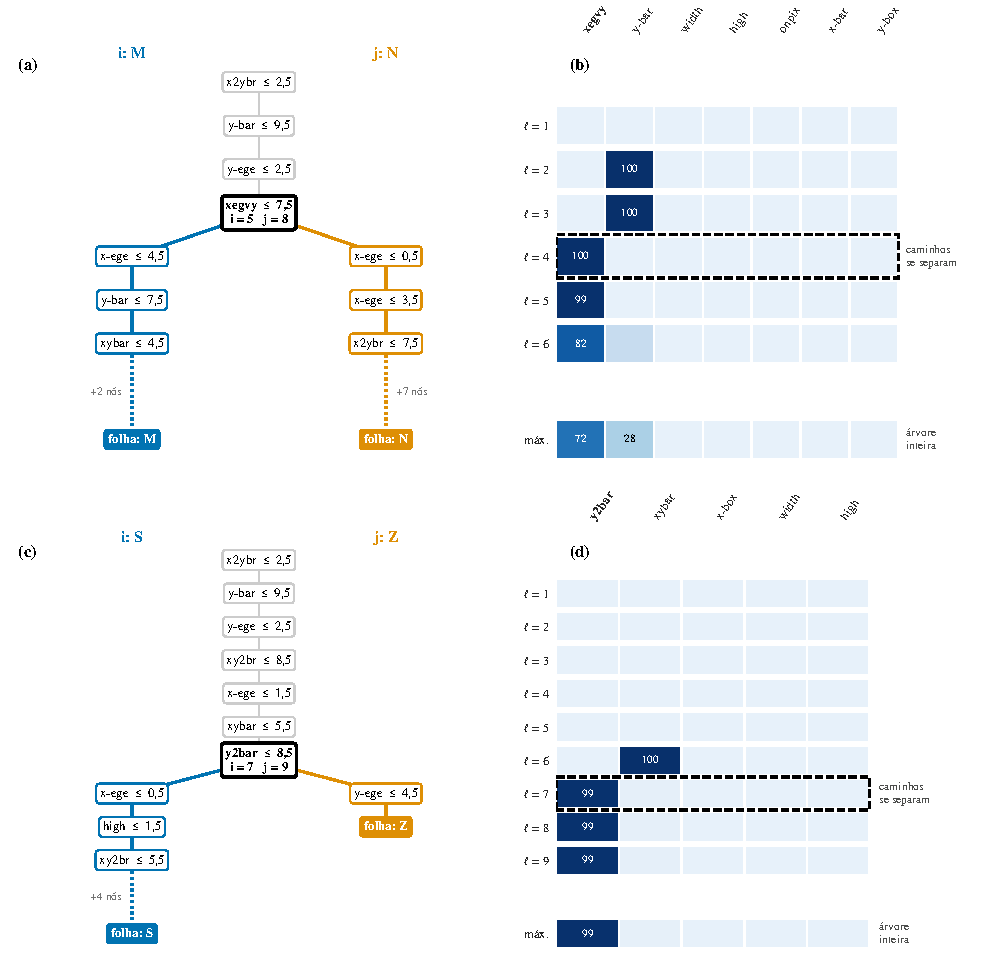
\includegraphics[width=\textwidth]{figuras/res_arvore_caminhos.pdf}
    \caption{A explicação da árvore de decisão e a leitura do método, lado a lado, para dois pares da \texttt{letter} (semente 0). (a, c) Caminhos das amostras $i$ (azul) e $j$ (laranja) na árvore: o trecho comum, o nó de separação (destacado, com os valores de $i$ e de $j$ no atributo testado) e os ramos até as folhas, com os nós intermediários omitidos. (b, d) Parcela de cada atributo, em porcentagem, na pontuação $\Delta d_f$ do método em cada profundidade $\ell$, alinhada verticalmente com a árvore. A linha tracejada marca a profundidade em que os caminhos se separam, e a última linha é a árvore inteira. As colunas são os atributos que diferem entre $i$ e $j$, na ordem do ranking final do método, e o atributo de separação está em negrito. Os dois pares ilustram o caso típico, em que a datação do método coincide com a da árvore (81\% dos pares).}
    \label{fig:res_arvore_caminhos}
\end{figure}

\begin{table}[htbp]
\centering
\caption{O método aplicado a uma árvore de decisão na \texttt{letter} (cinco sementes, cem pares por semente). Fração dos pares em que o atributo do nó em que os caminhos de $i$ e $j$ se separam é o primeiro de cada ranking, e área sob a curva do teste de trocas feito na própria árvore.}
\label{tab:res_arvore}
\small
\begin{tabular}{l c c}
\hline
Ranking & Corte da árvore em 1º & Área de trocas na árvore \\
\hline
\textbf{Método} (caminho $\circ$ folga $\circ$ classes) & $\mathbf{0{,}856}$ & $\mathbf{0{,}630}$ \\
Só caminho & $0{,}984$ & $0{,}628$ \\
Só folga & $0{,}852$ & $0{,}594$ \\
Só classes & $0{,}478$ & $0{,}603$ \\
Shapley exato com $j$ de referência & $0{,}766$ & $0{,}901$ \\
$|\Delta x|$ & $0{,}234$ & $0{,}716$ \\
Aleatória entre os que diferem & $0{,}132$ & $0{,}663$ \\
Método na árvore de rótulos embaralhados & $0{,}124$ & $0{,}466$ \\
\hline
\end{tabular}
\end{table}

\begin{figure}[htbp]
    \centering
    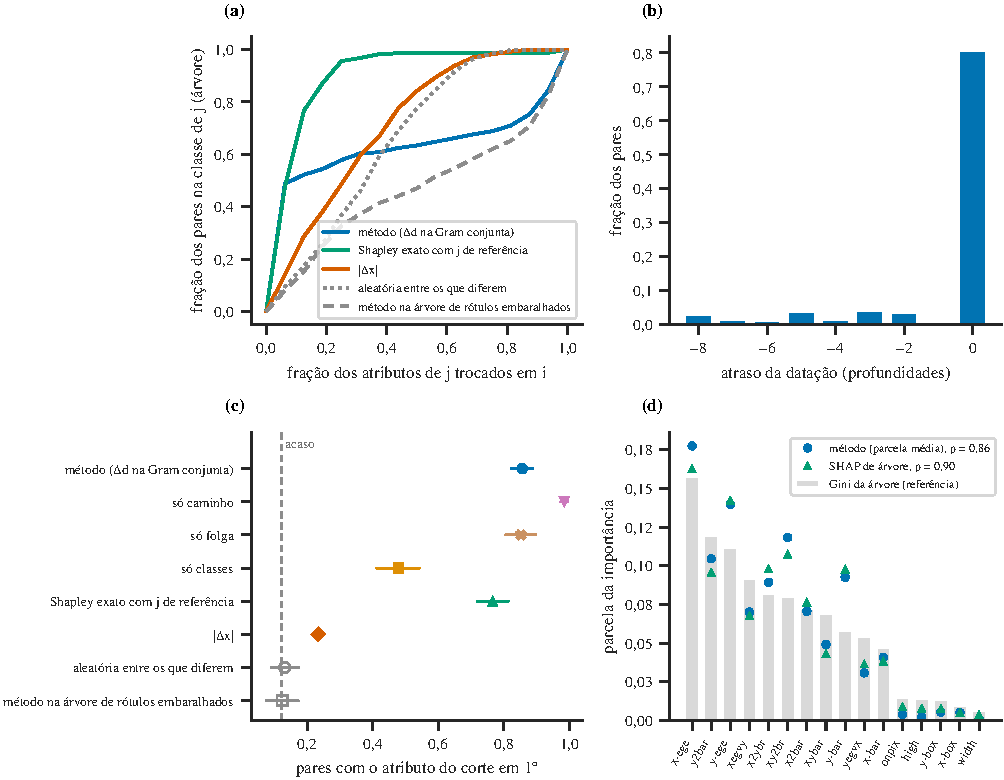
\includegraphics[width=\textwidth]{figuras/res_arvore.pdf}
    \caption{O método aplicado a uma árvore de decisão na \texttt{letter}. (a) Teste de trocas na própria árvore. (b) Diferença entre a profundidade em que o atributo de separação passa a ser o primeiro do método e a profundidade em que os caminhos de $i$ e $j$ se separam. (c) Fração dos pares em que o atributo de separação é o primeiro de cada ranking. (d) Importância global normalizada, na ordem da importância de Gini da árvore.}
    \label{fig:res_arvore}
\end{figure}

Em termos agregados (Tabela \ref{tab:res_arvore}), o atributo do nó de separação é o primeiro do método em 86\% dos pares, contra 77\% do Shapley exato, 23\% da diferença bruta e 12\% do piso. A fonte de caminho sozinha alcança 98\%, o que é quase uma consequência da construção, visto que trocar esse atributo é o que muda o caminho de $i$. O resultado não trivial é a datação: a profundidade em que o atributo de separação passa a ser o primeiro do método coincide com a profundidade da separação em 81\% dos pares e nunca ocorre depois dela (Figura \ref{fig:res_arvore}b). Nos demais pares, ela ocorre antes, quase sempre porque um nó acima da separação testa o mesmo atributo e a folga registra essa proximidade de um limiar. No nível global, a parcela média do método tem correlação de $0{,}86$ com a importância de Gini e de $0{,}94$ com o SHAP de árvore \citep{Lundberg2020}.

O mesmo experimento expõe o principal limite da leitura de pares. No teste de trocas na própria árvore, o método obtém $0{,}630$, abaixo da diferença bruta ($0{,}716$), e precisa, em média, de $5{,}8$ trocas para produzir um contrafactual válido, contra $1{,}7$ do contrafactual mínimo, obtido por enumeração. A causa é que $\Delta d_f$ troca um atributo de cada vez: os atributos que só importam depois que $i$ atravessa o corte não alteram nada quando trocados sozinhos, e ficam em ordem arbitrária no ranking. O valor de Shapley, que considera todas as combinações de trocas, enxerga essas interações. Sendo assim, a leitura de pares responde o que distingue $i$ do seu contrafactual, e não o menor conjunto de mudanças que basta para que $i$ se torne $j$.

\subsection{P8: Em que profundidade a decisão se forma?}\label{subsec:res_datacao}

A intervenção da Equação \eqref{eq:intervencao} fornece uma datação externa ao método: depois que a decisão está formada, o estado passa a ser redundante com ela e se torna robusto a perturbações. A correlação de Spearman entre essa estabilidade e a recuperação da decisão pela Gram conjunta é positiva em todas as bases tabulares, de $0{,}87 \pm 0{,}11$ na ResNet e de $1{,}00$ no transformador.

Essa concordância, entretanto, é mais fraca do que aparenta, pois as duas séries são monótonas na profundidade, e o valor observado decorre em boa medida dessa monotonicidade comum. O mesmo problema é conhecido nas sondagens lineares, em que a capacidade de decodificar uma propriedade cresce com a profundidade sem indicar onde o modelo a utiliza \citep{Belinkov2022}. Nas redes, a afirmação sustentada é apenas que as duas datações não se contradizem. A verificação genuína vem da árvore de decisão, em que a profundidade da decisão é conhecida para cada par e o método a acerta exatamente em 81\% dos pares.

\subsection{Custo computacional medido}\label{subsec:res_custo}

A análise da Subseção \ref{subsec:custo} foi verificada medindo o tempo de cada etapa enquanto o tamanho do problema cresce. Em escala logarítmica, um custo $\Theta(n^a)$ aparece como uma reta de inclinação $a$, e é essa inclinação que a Figura \ref{fig:res_complexidade} reporta.

\begin{figure}[htbp]
    \centering
    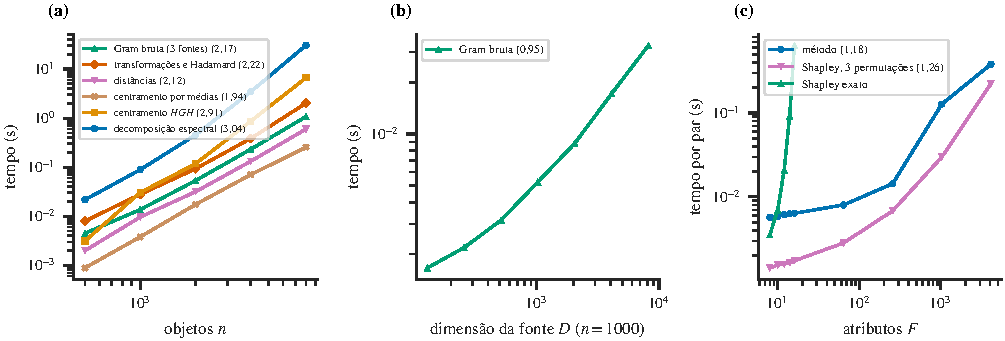
\includegraphics[width=\textwidth]{figuras/res_complexidade.pdf}
    \caption{Tempo das etapas do método em função do tamanho do problema, em escala logarítmica nos dois eixos. Entre parênteses está a inclinação ajustada nos três maiores tamanhos, que estima o expoente do custo. (a) Etapas da construção e das leituras em função do número de objetos $n$, com três fontes de dimensão 256. (b) Matriz de Gram bruta em função da dimensão $D$ da fonte, com $n = 1\,000$. (c) Leitura de diferenças entre pares em função do número de atributos $F$, comparada ao valor de Shapley exato com $j$ de referência e à sua estimativa por três permutações.}
    \label{fig:res_complexidade}
\end{figure}

Os expoentes medidos coincidem com os previstos. A matriz de Gram bruta cresce como $\Theta(n^2 D)$ (expoentes $2{,}17$ em $n$ e $0{,}95$ em $D$), as transformações, o produto de Hadamard e a matriz de distâncias crescem com expoente próximo de 2 e a decomposição espectral com $3{,}04$. As alternativas quadráticas da Tabela \ref{tab:custo} também se confirmam: o centramento pelas médias de linhas e colunas leva $0{,}25$ s com $n = 8\,000$, contra $6{,}6$ s do produto $H\widetilde{\mathbf{G}}H$. Com $n \approx 500$, entretanto, a decomposição leva cerca de $22$ ms, e o custo total é dominado pela extração das fontes. A leitura de pares confirma o custo linear no número de atributos (Figura \ref{fig:res_complexidade}c), enquanto o valor de Shapley exato dobra a cada atributo acrescentado. A sua estimativa por permutações, entretanto, também é linear e, por utilizar apenas passagens diretas, é mais rápida que o método por par.

\section{Discussão}\label{sec:discussao}

Esta seção discute \textit{por que} o método é capaz de fazer o que os resultados mostram, e por que deixa de ser capaz em outros casos. As propriedades da construção são garantidas pela teoria, e o que se discute a seguir diz respeito, salvo menção contrária, à instanciação, isto é, a se uma escolha particular de fontes produz um espaço que reflete o modelo.

\subsection{A estrutura do espaço de representação, bloco a bloco}\label{subsec:disc_espaco}

Como a matriz de Gram é semidefinida positiva, cada objeto admite uma realização $\varphi_i$ com $G_{ij} = \langle \varphi_i, \varphi_j \rangle$ (Equação \eqref{eq:empirical_feature_realization}), e as coordenadas associadas aos dois maiores autovalores, $\bigl(\sqrt{\hat\lambda_1}\,V_{i1}, \sqrt{\hat\lambda_2}\,V_{i2}\bigr)$, formam a projeção plana que preserva a maior parte da energia do espaço, sem nenhum parâmetro adicional. A Figura \ref{fig:disc_espaco} mostra essa projeção em todos os blocos do perceptron multicamadas treinado sobre a base \texttt{segment}, que tem sete classes, poucas o bastante para serem distinguidas por cor.

\begin{figure}[htbp]
  \centering
  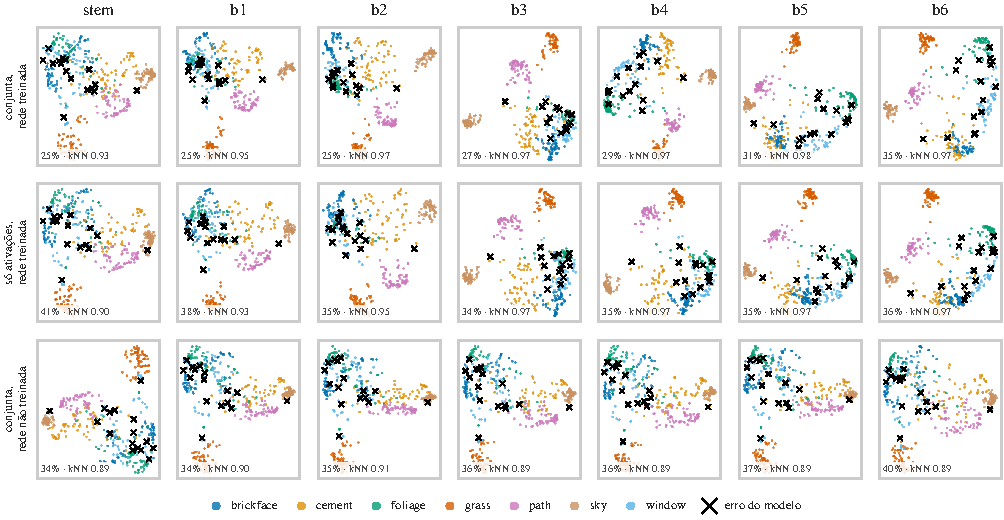
\includegraphics[width=\textwidth]{figuras/disc_espaco.pdf}
  \caption{O espaço de representação bloco a bloco, projetado nos seus dois modos dominantes, sobre as 462 amostras de teste da \texttt{segment} (perceptron multicamadas, semente 0, alvo fixo). A primeira linha mostra a Gram conjunta da rede treinada, a segunda apenas a fonte de ativações, com a mesma transformação das componentes, e a terceira a Gram conjunta da rede não treinada, com os mesmos pesos iniciais. A cor é a classe predita pela rede treinada, e os $\times$ marcam as amostras que ela erra. No canto de cada painel estão a fração da energia retida pelos dois eixos e o acerto do $k$-vizinhos contra a predição, calculado sobre a matriz de Gram inteira, e não sobre o plano.}
  \label{fig:disc_espaco}
\end{figure}

Três aspectos da figura ajudam a entender os resultados. O primeiro é o contraste entre a rede treinada e a não treinada. Na rede não treinada (terceira linha), a geometria é praticamente a mesma em todos os blocos: a rede aleatória apenas propaga a estrutura da entrada, e as classes que já são separáveis nos atributos brutos, como \texttt{grass} e \texttt{sky}, aparecem isoladas desde o \texttt{stem}. É exatamente essa separabilidade herdada da entrada que torna o piso cruzado alto nas bases tabulares, com $k$-vizinhos em torno de $0{,}89$ nesta base. Na rede treinada (primeira linha), ao contrário, a geometria muda a cada bloco: \texttt{path}, \texttt{grass} e \texttt{sky} se destacam em grupos compactos a partir de \texttt{b3}, e as classes que a rede tem mais dificuldade de separar, \texttt{brickface}, \texttt{foliage}, \texttt{window} e \texttt{cement}, passam a ocupar uma região comum. O que distingue a medida do seu piso é, portanto, a reorganização produzida pelo treinamento, e não a separabilidade dos dados.

O segundo aspecto é a posição dos erros. Os objetos que o modelo erra não estão espalhados pelo espaço: eles se concentram na região em que as classes confundíveis se encontram, e isso ocorre em todos os blocos da rede treinada. Essa é a razão pela qual a margem geométrica prevê o acerto (P1). Um objeto cuja vizinhança mistura predições diferentes está, geometricamente, em uma fronteira, e é nas fronteiras que o modelo erra. Veja que o método não recebe o rótulo verdadeiro em nenhum momento, de modo que essa concentração é uma propriedade do espaço construído, e não da forma como ele foi desenhado.

O terceiro aspecto é a comparação entre a composição e a fonte de ativações isolada (segunda linha). Nesta base tabular, as duas geometrias são parecidas, e a composição só se distingue nos blocos rasos, o padrão que P2 encontrou nas bases tabulares. Por fim, é preciso ler a figura com uma cautela: os dois eixos retêm apenas de 25\% a 40\% da energia, de modo que objetos sobrepostos no plano podem estar separados nas demais dimensões, e é por esse motivo que o acerto do $k$-vizinhos é calculado sobre a matriz inteira.

\subsection{O que o método é capaz de fazer, e por quê}\label{subsec:res_instanciacao}

\textbf{Refletir a decisão e o erro.} A primeira capacidade demonstrada é a de construir um espaço em que a vizinhança de um objeto antecipa como o modelo o trata. A razão está na forma multiplicativa da composição. Como discutido no Comentário \ref{rem:joint_similarity}, o produto de Hadamard impõe um critério de similaridade conjunta: dois objetos só são próximos se forem próximos em todas as fontes simultaneamente. Na instanciação utilizada, isso significa que dois objetos vizinhos têm estados parecidos, ativam filtros parecidos \textit{e} têm a decisão sensível às mesmas direções. Vizinhos nesse espaço compartilham, portanto, não apenas o conteúdo, mas a razão pela qual o modelo os trataria da mesma forma, e é essa propriedade que permite usar a vizinhança como indício de confiança, como fazem o \textit{trust score} e os $k$-vizinhos profundos \citep{Jiang2018, Papernot2018}.

\textbf{Acrescentar algo às ativações onde elas ainda não decidem.} A composição supera a fonte de ativações nos blocos rasos e intermediários e se iguala a ela na saída da rede, e a diferença é muito maior na ResNet do que no perceptron multicamadas. A explicação é que as ativações descrevem o que a rede \textit{vê}, enquanto o gradiente contrastivo descreve o que \textit{importaria} para a decisão. Nos blocos profundos, as ativações das amostras de uma mesma classe tendem a colapsar em torno de uma média de classe \citep{Papyan2020} e passam a carregar a decisão por si mesmas, de modo que a composição deixa de ter o que acrescentar. No perceptron multicamadas, cuja entrada já é quase separável, e no transformador, cujo gradiente quase não carrega informação sobre a decisão, a vantagem é pequena ou inexistente. Veja que isso delimita a instanciação, e não o método: a contribuição de cada fonte é uma propriedade do modelo analisado, e outra escolha de fontes pode ser mais informativa em outra arquitetura.

\textbf{Ver o que a CKA não vê.} A decomposição contra a CKA mostrou que a parte da Gram vista pela CKA coincide com a geometria euclidiana das ativações, de modo que a parte residual é exatamente o que uma análise das ativações não enxerga. Essa parte residual prevê o acerto melhor do que a vista nos blocos rasos e intermediários da ResNet e pior nas bases tabulares e no transformador. Veja que esse é o mesmo padrão da capacidade anterior, e pela mesma razão: o que o método vê além da CKA é, essencialmente, a contribuição do gradiente. Sendo assim, o método se distingue da CKA exatamente onde a sensibilidade da decisão diverge do conteúdo das ativações.

\textbf{Concentrar a decisão em poucas direções.} A leitura espectral mais robusta é a contenção das direções de classe no subespaço retido, em que a composição supera as ativações em toda a profundidade, nas bases tabulares e nas duas arquiteturas. Isso significa que as poucas direções dominantes do espaço construído são as direções em que o modelo separa as suas decisões. A razão de energia ortogonal, que mede quanto de cada objeto vive fora dessas direções, só é confiável quando o subespaço retido já é o subespaço da decisão, isto é, nos blocos profundos da ResNet e em quase todos os blocos do transformador. Em outras palavras, a energia que escapa de $V_r$ sinaliza uma amostra que o modelo não sabe representar apenas quando $V_r$ é o espaço em que o modelo decide, a mesma condição que torna útil o resíduo do subespaço principal na detecção de amostras fora da distribuição \citep{Wang2022ViM}.

\textbf{Localizar sem necessariamente explicar.} Sobre a entrada, o campo de energia da ResNet localiza o animal muito melhor do que um mapa centrado e do que o Grad-CAM, mas ordena a evidência da decisão pior do que o Grad-CAM nos blocos profundos. A diferença entre as duas tarefas explica o resultado. A energia de uma posição mede o quanto ela participa dos modos dominantes da geometria da imagem, isto é, da estrutura que o modelo representa, enquanto o Grad-CAM pondera cada posição diretamente pela sensibilidade da decisão. Um mapa de estrutura cobre o objeto inteiro, enquanto um mapa de sensibilidade ordena as suas partes pela importância. No transformador, nem a localização se sustenta, porque a atenção mistura informação de toda a imagem desde as primeiras camadas \citep{Raghu2021}, e a posição deixa de ser uma unidade natural de objeto. Na prática, o campo de energia é útil para auditar \textit{onde} uma rede convolucional representa o objeto, por exemplo para detectar um modelo que se apoia no fundo \citep{Geirhos2020}, mas não substitui um mapa de relevância quando a pergunta é quais partes sustentam a decisão.

\textbf{Explicar por contrafactuais, inclusive fora das redes neurais.} A leitura de pares responde à pergunta contrastiva, ``por que esta amostra e não aquela?'', que é a forma natural das explicações humanas \citep{Miller2019}, e o faz tomando como referência um contrafactual no sentido de \cite{Guidotti2022}: a amostra observada mais próxima que o modelo decide de outra forma. A distância do método entra em dois pontos. Ela ordena as diferenças entre a amostra e o seu contrafactual pelo quanto cada uma aproxima as duas no espaço do modelo, e cada pontuação $\Delta d_f$ é o efeito de uma intervenção $do(x_f := x_{j,f})$ sobre essa distância. É por isso que o método supera o SHAP e o LIME nas formas em que eles são usualmente aplicados, que explicam uma amostra em relação a uma referência genérica, e não em relação ao contrafactual. O resultado mais forte, entretanto, vem da árvore de decisão, em que a resposta certa é conhecida e o método a recupera sem receber a regra de decisão, apenas trocando as fontes. Esse é o argumento mais direto de que o método é modelo-agnóstico: a construção exige somente que cada amostra possa ser descrita por fontes sobre as quais se define um \textit{kernel}, e o que depende do modelo é apenas a instanciação.

\textbf{Datar a decisão.} As leituras por bloco produzem uma datação da decisão, e nas redes essa datação concorda com a obtida por intervenção sobre os estados internos. Essa concordância, contudo, decorre em boa parte de as duas séries crescerem com a profundidade, e por isso ela não é, sozinha, uma validação. A validação veio da árvore, em que a profundidade da decisão é conhecida para cada par. Uma consequência prática é que a leitura por bloco permite localizar em que ponto da rede uma distinção passa a ser usada, como no par da \texttt{letter} em que a dispersão horizontal da letra só pesa no meio da rede, uma informação que atribuições sobre a saída do modelo não oferecem.

\subsection{Quando o método não é capaz, e por quê}\label{subsec:disc_limites}

Três limites decorrem da própria construção das leituras, e não de detalhes de implementação.

O primeiro é que a leitura de pares é de primeira ordem. A pontuação $\Delta d_f$ intervém em um atributo de cada vez, e os atributos que só importam em conjunto não mudam nada quando trocados sozinhos. Por isso o método recupera o atributo que separa a amostra do seu contrafactual, mas não o contrafactual mínimo, isto é, o menor conjunto de mudanças que altera a decisão, e o valor de Shapley com $j$ de referência, que considera todas as combinações de trocas, o supera no teste de trocas. Em outras palavras, o método explica o que distingue duas instâncias, e não como transformar uma na outra com o menor custo, que é o objetivo dos geradores de contrafactuais \citep{Wachter2018, Guidotti2022}. Uma extensão natural do método é substituir a troca isolada por trocas sequenciais, recalculando a distância depois de cada uma, o que capturaria interações e manteria o custo linear no número de atributos.

O segundo é que o método depende de o treinamento reorganizar a geometria. Se a tarefa é resolvida quase na entrada, a rede treinada e a não treinada produzem espaços parecidos, e as leituras se aproximam do que a diferença bruta entre as amostras já dizia. É o que se observa nas bases tabulares, em que o piso cruzado é alto e a leitura de pares empata com a diferença bruta $|\Delta x|$, e é coerente com a Figura \ref{fig:disc_espaco}, em que a vantagem sobre o piso é justamente a reorganização entre os blocos. A similaridade entre a Gram da rede treinada e a da rede na inicialização é barata e poderia ser reportada antes de qualquer leitura, como um diagnóstico de aplicabilidade, mas esse critério ainda precisa ser validado sobre um número maior de bases.

O terceiro é que a validade das leituras referidas à decisão depende da escolha do alvo do gradiente. Com a classe predita como alvo, o gradiente carrega a própria predição, e as leituras de decisão se tornam circulares, chegando a recuperar a predição em mais de 95\% dos casos já em \texttt{b3} da ResNet. O alvo fixo remove essa circularidade ao custo de tornar o gradiente degenerado no último bloco. Essa é uma restrição da fonte de gradiente, e não do método, mas qualquer instanciação que utilize a decisão como fonte precisa de um controle equivalente.

\subsection{Limitações e trabalhos futuros}\label{subsec:res_limitacoes}

A proposição de que as distâncias do espaço de representação refletem o entendimento que o modelo tem dos dados foi avaliada apenas em sua dimensão comportamental. Nenhuma referência semântica externa ao modelo, como uma hierarquia de superclasses ou julgamentos humanos de similaridade, foi utilizada, de modo que a afirmação de que as distâncias representam diferenças semânticas permanece sem teste.

Do ponto de vista experimental, quatro limitações devem ser registradas. A base de imagens impõe um regime de dados escassos, com cerca de noventa imagens por raça, o que limita a acurácia dos modelos treinados do zero, sobretudo a do transformador. Treinar a partir de pesos pré-treinados elevaria essa acurácia, mas descaracterizaria o piso, que é a mesma rede na inicialização. As comparações são reportadas pela média, pelo desvio e pela fração das execuções em que se sustentam, sem testes de hipótese. Testes pareados ao nível dos pares, como o de postos sinalizados de Wilcoxon com correção para comparações múltiplas, e o teste de Friedman entre bases seriam os adequados a este desenho. A leitura de previsão do acerto não foi comparada à confiança do próprio \textit{softmax}, e os estudos de caso utilizam uma única base. Por fim, os conjuntos de nível foram validados apenas na ResNet, o piso adotado na diagonal da transformação angular não foi variado e a seleção da posição de referência ainda não exclui a borda da imagem.

Além das extensões já mencionadas, a leitura de pares por trocas sequenciais e a decomposição espectral truncada para amostras maiores, duas direções decorrem diretamente da separação entre método e instanciação. A primeira é explorar outras fontes para as arquiteturas em que o gradiente pouco contribui, como o transformador, em que a atenção é uma candidata natural a fonte. A segunda é utilizar o método para comparar modelos diferentes sobre as mesmas amostras, como a árvore de decisão e o perceptron multicamadas da \texttt{letter}, colocando os dois na mesma geometria e perguntando não apenas se eles usam os mesmos atributos, mas se organizam os dados da mesma forma.


\bibliographystyle{plainnat}
\bibliography{referencias}

% O apendice ainda contem tabelas da versao anterior (CIFAR-10) e fica fora da compilacao
% ate ser refeito com os experimentos atuais; nenhum texto do corpo faz referencia a ele.
% \appendix

\section{Valores numéricos dos resultados}\label{sec:apendice_tabelas}

% PENDENTE (2026-09-25): as tabelas deste apendice ainda sao as da rodada preliminar
% (CIFAR-10 e Cat/Dog, uma unica semente) e precisam ser regeradas a partir de
% `outputs/tabular_suite/tables_fixed.md`, `outputs/pets_suite/tables_fixed.md`,
% `outputs/pets_regions/tables.md` e `outputs/tabular_differences/tables.md`.
Este apêndice reúne os valores numéricos das leituras apresentadas na Seção \ref{sec:resultados}, por bloco da rede.

\begin{table}[htbp]
\centering
\caption{Leituras da matriz de distância referidas ao comportamento da rede, por bloco. O piso é o controle cruzado: a geometria da rede não treinada medida contra o comportamento da rede treinada.}
\label{tab:res_distancia}
\resizebox{\textwidth}{!}{%
\begin{tabular}{llccccccc}
\hline
Leitura & Representação & \texttt{stem} & \texttt{b1} & \texttt{b2} & \texttt{b3} & \texttt{b4} & \texttt{b5} & \texttt{b6} \\
\hline
\multirow{5}{*}{$k$-vizinhos contra a predição} & Gram conjunta & 0,296 & 0,512 & 0,644 & 0,856 & 0,946 & 1,000 & 1,000 \\
 & Gradiente ($\Gamma$) & 0,178 & 0,384 & 0,530 & 0,800 & 0,932 & 1,000 & 1,000 \\
 & Ativações ($A$) & 0,288 & 0,382 & 0,524 & 0,580 & 0,704 & 0,918 & 0,984 \\
 & RSA euclidiana & 0,264 & 0,374 & 0,484 & 0,564 & 0,636 & 0,768 & 0,986 \\
 & Piso cruzado & 0,300 & 0,302 & 0,294 & 0,310 & 0,306 & 0,272 & 0,254 \\
\hline
\multirow{5}{*}{AUC da margem para o acerto} & Gram conjunta & 0,580 & 0,764 & 0,834 & 0,879 & 0,982 & 1,000 & 1,000 \\
 & Gradiente ($\Gamma$) & 0,659 & 0,783 & 0,870 & 0,939 & 0,980 & 1,000 & 1,000 \\
 & Ativações ($A$) & 0,556 & 0,590 & 0,642 & 0,712 & 0,764 & 0,937 & 0,999 \\
 & RSA euclidiana & 0,503 & 0,524 & 0,593 & 0,635 & 0,695 & 0,805 & 0,999 \\
 & Piso cruzado & 0,562 & 0,554 & 0,552 & 0,535 & 0,534 & 0,523 & 0,520 \\
\hline
\multirow{5}{*}{Spearman com a confusão} & Gram conjunta & 0,375 & 0,292 & 0,366 & 0,243 & 0,426 & 0,575 & 0,742 \\
 & Gradiente ($\Gamma$) & $-$0,005 & 0,009 & $-$0,094 & $-$0,103 & $-$0,090 & 0,173 & 0,775 \\
 & Ativações ($A$) & 0,418 & 0,329 & 0,366 & 0,282 & 0,506 & 0,634 & 0,635 \\
 & RSA euclidiana & 0,444 & 0,491 & 0,363 & 0,298 & 0,488 & 0,435 & 0,516 \\
 & Piso cruzado & 0,101 & 0,060 & 0,092 & 0,089 & 0,095 & 0,085 & 0,078 \\
\hline
\end{tabular}}
\end{table}

\begin{table}[htbp]
\centering
\caption{Leituras espectrais por bloco. A contenção é a fração das direções de classe dentro de $V_r$; o coeficiente de variação (CV) e a AUC referem-se à razão de energia ortogonal $\widehat{E}_{\mathrm{ratio}}$. O controle é a Gram conjunta da rede não treinada.}
\label{tab:res_espectro}
\resizebox{\textwidth}{!}{%
\begin{tabular}{llccccccc}
\hline
Leitura & Representação & \texttt{stem} & \texttt{b1} & \texttt{b2} & \texttt{b3} & \texttt{b4} & \texttt{b5} & \texttt{b6} \\
\hline
\multirow{4}{*}{Contenção das classes em $V_r$} & Gram conjunta & 0,440 & 0,625 & 0,647 & 0,838 & 0,873 & 0,916 & 0,915 \\
 & Gradiente ($\Gamma$) & 0,313 & 0,451 & 0,422 & 0,608 & 0,747 & 0,890 & 0,903 \\
 & Ativações ($A$) & 0,138 & 0,265 & 0,306 & 0,493 & 0,599 & 0,787 & 0,871 \\
 & Controle & 0,146 & 0,136 & 0,122 & 0,087 & 0,071 & 0,062 & 0,032 \\
\hline
\multirow{2}{*}{CV de $\widehat{E}_{\mathrm{ratio}}$} & Gram conjunta & 0,066 & 0,058 & 0,055 & 0,103 & 0,087 & 0,140 & 0,400 \\
 & Controle & 0,225 & 0,237 & 0,259 & 0,329 & 0,351 & 0,400 & 0,435 \\
\hline
\multirow{4}{*}{AUC de $\widehat{E}_{\mathrm{ratio}}$ para o erro} & Gram conjunta & 0,523 & 0,404 & 0,540 & 0,581 & 0,528 & 0,687 & 0,811 \\
 & Gradiente ($\Gamma$) & 0,369 & 0,371 & 0,338 & 0,236 & 0,181 & 0,316 & 0,893 \\
 & Ativações ($A$) & 0,472 & 0,510 & 0,593 & 0,556 & 0,548 & 0,795 & 0,737 \\
 & Controle & 0,555 & 0,550 & 0,567 & 0,544 & 0,550 & 0,556 & 0,605 \\
\hline
\end{tabular}}
\end{table}

\begin{table}[htbp]
\centering
\caption{Fração de predições alteradas pela intervenção em cada bloco, para diferentes orçamentos relativos $\sigma$.}
\label{tab:res_flip}
\resizebox{\linewidth}{!}{%
\begin{tabular}{lccccccc}
\hline
Orçamento & \texttt{stem} & \texttt{b1} & \texttt{b2} & \texttt{b3} & \texttt{b4} & \texttt{b5} & \texttt{b6} \\
\hline
$\sigma = 1$ & 0,110 & 0,058 & 0,026 & 0,032 & 0,024 & 0,026 & 0,004 \\
$\sigma = 2$ & 0,422 & 0,216 & 0,150 & 0,350 & 0,098 & 0,058 & 0,008 \\
$\sigma = 4$ & 0,880 & 0,716 & 0,722 & 0,826 & 0,790 & 0,234 & 0,012 \\
Não treinada, $\sigma = 2$ & 0,210 & 0,208 & 0,214 & 0,212 & 0,242 & 0,118 & 0,146 \\
\hline
\end{tabular}}
\end{table}

\begin{table}[htbp]
\centering
\caption{Decomposição da Gram do método contra a Gram das ativações da mesma camada. As duas últimas leituras tratam cada parte da decomposição como uma geometria própria, após a projeção no cone semidefinido positivo.}
\label{tab:res_cka}
\resizebox{\textwidth}{!}{%
\begin{tabular}{llccccccc}
\hline
Leitura & Representação & \texttt{stem} & \texttt{b1} & \texttt{b2} & \texttt{b3} & \texttt{b4} & \texttt{b5} & \texttt{b6} \\
\hline
\multirow{4}{*}{Alinhamento $a$} & Ativações ($A$), âncora & 0,977 & 0,985 & 0,995 & 0,992 & 0,994 & 0,937 & 0,987 \\
 & Parâmetros ($W$) & 0,893 & 0,961 & 0,959 & 0,970 & 0,962 & 0,918 & 0,965 \\
 & Gram conjunta & 0,700 & 0,467 & 0,579 & 0,691 & 0,676 & 0,843 & 0,932 \\
 & Gradiente ($\Gamma$) & 0,089 & 0,155 & 0,152 & 0,246 & 0,301 & 0,595 & 0,867 \\
\hline
\multirow{2}{*}{$k$-vizinhos contra a predição} & Parte vista pela CKA & 0,264 & 0,374 & 0,484 & 0,564 & 0,636 & 0,768 & 0,986 \\
 & Parte residual & 0,202 & 0,334 & 0,482 & 0,652 & 0,858 & 0,886 & 1,000 \\
\hline
\multirow{2}{*}{AUC da margem para o acerto} & Parte vista pela CKA & 0,503 & 0,524 & 0,593 & 0,635 & 0,695 & 0,805 & 0,999 \\
 & Parte residual & 0,658 & 0,802 & 0,815 & 0,857 & 0,929 & 0,990 & 1,000 \\
\hline
Massa espectral descartada & Parte residual & 0,034 & 0,022 & 0,025 & 0,039 & 0,064 & 0,147 & 0,482 \\
\hline
\end{tabular}}
\end{table}

\begin{table}[htbp]
\centering
\caption{Diferença entre as áreas sob a curva da margem normalizada ao remover os píxeis do menos para o mais relevante e do mais para o menos relevante, por bloco. Nas duas primeiras leituras a relevância é a energia do campo; na última, a proximidade a $s_0$. O piso cruzado é a mesma ordenação calculada na rede não treinada e aplicada à rede treinada; a ordem aleatória resulta em $0{,}001$ no CIFAR-10 e em $0{,}006$ na base de gatos e cachorros. Em \texttt{b6} o campo do gradiente isolado é indefinido.}
\label{tab:res_campo}
\resizebox{\textwidth}{!}{%
\begin{tabular}{llccccccc}
\hline
Leitura & Representação & \texttt{stem} & \texttt{b1} & \texttt{b2} & \texttt{b3} & \texttt{b4} & \texttt{b5} & \texttt{b6} \\
\hline
\multirow{6}{*}{Campo de energia, CIFAR-10} & Gram conjunta & 0,181 & 0,220 & 0,264 & 0,299 & 0,323 & 0,361 & 0,159 \\
 & Ativações ($A$) & 0,146 & 0,148 & 0,150 & 0,177 & 0,232 & 0,398 & 0,196 \\
 & Parâmetros ($W$) & 0,139 & 0,106 & 0,122 & 0,188 & 0,244 & 0,396 & 0,081 \\
 & Gradiente ($\Gamma$) & 0,103 & 0,211 & 0,239 & 0,304 & 0,289 & 0,303 & -- \\
 & Grad-CAM & 0,002 & 0,020 & $-$0,025 & 0,057 & 0,050 & 0,171 & 0,422 \\
 & Piso cruzado & 0,074 & 0,060 & 0,051 & 0,066 & 0,065 & 0,043 & 0,023 \\
\hline
\multirow{6}{*}{Campo de energia, gatos e cachorros} & Gram conjunta & 0,290 & 0,386 & 0,327 & 0,315 & 0,580 & 0,522 & 0,279 \\
 & Ativações ($A$) & 0,058 & 0,136 & 0,155 & 0,222 & 0,459 & 0,295 & 0,302 \\
 & Parâmetros ($W$) & 0,066 & 0,143 & 0,199 & 0,293 & 0,556 & 0,329 & 0,262 \\
 & Gradiente ($\Gamma$) & 0,328 & 0,392 & 0,381 & 0,380 & 0,435 & 0,251 & -- \\
 & Grad-CAM & $-$0,093 & $-$0,080 & 0,020 & 0,154 & 0,319 & 0,558 & 0,896 \\
 & Piso cruzado & 0,221 & 0,202 & 0,226 & 0,223 & 0,197 & 0,057 & 0,025 \\
\hline
\multirow{3}{*}{Distância a $s_0$, gatos e cachorros} & Pseudodistância original & $-$0,157 & $-$0,147 & $-$0,075 & $-$0,112 & $-$0,332 & 0,162 & 0,935 \\
 & Distância angular & $-$0,029 & 0,120 & 0,214 & $-$0,042 & 0,695 & 0,630 & 0,677 \\
 & Piso cruzado (angular) & 0,176 & 0,180 & 0,190 & 0,143 & 0,145 & 0,080 & 0,086 \\
\hline
\end{tabular}}
\end{table}

\section{Diagnósticos da variante com raiz $d$-ésima}\label{sec:apendice_raiz}

Esta seção reúne os diagnósticos da variante da Equação \eqref{eq:raiz}, em que o produto de Hadamard das componentes é substituído pela sua média geométrica. Esses diagnósticos não testam a proposição do trabalho, mas verificam se a variante se comporta como a teoria prevê e em quais leituras ela deve ser utilizada. A Tabela \ref{tab:apendice_raiz} reúne os valores discutidos a seguir.

\begin{table}[htbp]
\centering
\caption{Comparação entre a Gram conjunta pelo produto de Hadamard e pela raiz $d$-ésima, por bloco.}
\label{tab:apendice_raiz}
\resizebox{\textwidth}{!}{%
\begin{tabular}{llccccccc}
\hline
Quantidade & Composição & \texttt{stem} & \texttt{b1} & \texttt{b2} & \texttt{b3} & \texttt{b4} & \texttt{b5} & \texttt{b6} \\
\hline
\multirow{5}{*}{Mediana fora da diagonal} & Componente $A$ & 0,905 & 0,920 & 0,892 & 0,765 & 0,781 & 0,620 & 0,621 \\
 & Componente $W$ & 0,827 & 0,926 & 0,870 & 0,809 & 0,832 & 0,698 & 0,761 \\
 & Componente $\Gamma$ & 0,500 & 0,501 & 0,502 & 0,504 & 0,509 & 0,559 & 0,445 \\
 & Produto & 0,370 & 0,424 & 0,387 & 0,309 & 0,329 & 0,238 & 0,210 \\
 & Raiz & 0,718 & 0,751 & 0,729 & 0,676 & 0,690 & 0,620 & 0,594 \\
\hline
Spearman entre as distâncias & Produto e raiz & 0,9992 & 0,9988 & 0,9990 & 1,0000 & 0,9998 & 1,0000 & 1,0000 \\
\hline
\multirow{2}{*}{Violação da semidefinição positiva} & Massa espectral negativa & 0,51\% & 0,37\% & 0,41\% & 0,003\% & 0,04\% & 0 & 0 \\
 & Autovalores negativos & 125 & 101 & 110 & 2 & 10 & 0 & 0 \\
\hline
\multirow{2}{*}{Modos ativos $r$} & Produto & 132 & 193 & 169 & 243 & 204 & 88 & 16 \\
 & Raiz & 73 & 130 & 105 & 145 & 122 & 49 & 13 \\
\hline
\multirow{2}{*}{Fidelidade da projeção 2D} & Produto & 0,076 & 0,040 & 0,052 & 0,038 & 0,042 & 0,095 & 0,186 \\
 & Raiz & 0,112 & 0,052 & 0,071 & 0,057 & 0,059 & 0,134 & 0,211 \\
\hline
\multirow{2}{*}{Energia de classe (múltiplo do acaso)} & Produto & 2,3 & 2,1 & 2,7 & 2,9 & 4,0 & 13,6 & 38,1 \\
 & Raiz & 2,8 & 2,4 & 3,2 & 3,7 & 5,1 & 18,4 & 42,3 \\
\hline
\multirow{2}{*}{Contenção das classes em $V_r$} & Produto & 0,440 & 0,625 & 0,647 & 0,838 & 0,873 & 0,916 & 0,915 \\
 & Raiz & 0,289 & 0,504 & 0,506 & 0,706 & 0,800 & 0,897 & 0,912 \\
\hline
\multirow{2}{*}{Silhueta} & Produto & $-$0,007 & $-$0,001 & 0,002 & 0,007 & 0,018 & 0,111 & 0,439 \\
 & Raiz & $-$0,010 & $-$0,001 & 0,003 & 0,009 & 0,025 & 0,153 & 0,505 \\
\hline
\multirow{2}{*}{Spearman com a confusão} & Produto & 0,375 & 0,292 & 0,366 & 0,243 & 0,426 & 0,575 & 0,742 \\
 & Raiz & 0,342 & 0,284 & 0,326 & 0,220 & 0,394 & 0,562 & 0,697 \\
\hline
\end{tabular}}
\end{table}

O encolhimento multiplicativo previsto no Comentário \ref{rem:joint_similarity} é observado diretamente. Com componentes cujas medianas fora da diagonal ficam entre $0{,}45$ e $0{,}93$, o produto das três resulta em medianas entre $0{,}21$ e $0{,}42$, e a raiz devolve esses valores à escala das componentes, entre $0{,}59$ e $0{,}75$. Esse encolhimento é a causa direta do elevado número de modos ativos e da baixa fidelidade da projeção discutidos na Subseção \ref{subsec:res_instanciacao}.

A correlação de Spearman entre as distâncias do produto e as da raiz é de no mínimo $0{,}9988$, o que confirma que a raiz preserva a ordenação das distâncias. Sendo assim, nenhuma leitura baseada em postos, como $k$-vizinhos, área sob a curva ROC e correlações de Spearman, pode ser alterada de forma relevante pela raiz, e a estabilidade dessas leituras sob a variante não constitui evidência a seu favor.

Quanto à semidefinição positiva, a potência de Hadamard fracionária não é garantida pelo teorema de Schur. Pelo resultado de \citet{FitzGeraldHorn1977}, $\mathbf{A}^{\circ p}$ é semidefinida positiva para toda matriz semidefinida positiva de entradas não negativas de ordem $n$ se e somente se $p \geq n-2$ ou $p$ é inteiro, e com $p = 1/3$ e $n = 500$ essa garantia não existe. A violação medida, entretanto, é pequena: a massa espectral negativa é de no máximo 0,51\% nos blocos rasos, com menor autovalor de $-0{,}068$, e desaparece a partir de \texttt{b5}, em que a matriz resultante já é semidefinida positiva sem nenhuma projeção.

As quantidades que dependem dos valores das entradas, e não da sua ordenação, são as que a raiz de fato altera. O número de modos ativos cai entre 19\% e 45\%, a fidelidade da projeção em duas dimensões aumenta entre 13\% e 50\% em termos relativos, a energia de classe aumenta entre 11\% e 35\% e a silhueta em \texttt{b6} passa de $0{,}439$ para $0{,}505$. Por outro lado, a raiz reduz a contenção das direções de classe em $V_r$ em todos os blocos, sobretudo nos rasos ($0{,}440$ para $0{,}289$ em \texttt{stem}), e reduz levemente a concordância com a confusão, de $0{,}742$ para $0{,}697$ em \texttt{b6}. Veja que a contenção depende de $V_r$ e, portanto, do número de modos retidos, que é justamente o que a raiz modifica.

Sendo assim, a variante com raiz é recomendada quando a afirmação é espectral ou visual, como na análise da energia por modo e na produção de dispersogramas, enquanto o produto de Hadamard deve ser mantido nas leituras de comportamento e de contenção, que são as leituras sancionadas pela teoria sem ressalvas.

\section{Verificação da energia na Gram bruta e na Gram transformada}\label{sec:apendice_bruta}

A aritmética da energia espectral é exata para qualquer matriz simétrica, mas a transformação $T$ altera o objeto cuja norma está sendo medida. Na Gram bruta, a energia de cada amostra é a norma no RKHS no sentido estrito, mas a normalização angular fixa essa norma em 1 para todas as amostras, e por isso a razão $\widehat{E}_{\mathrm{ratio}}$ só é informativa por medir direção, e não magnitude. Duas propriedades foram verificadas. A primeira é que o alinhamento espectral com a classe, como múltiplo do acaso, é idêntico nas duas matrizes em todos os blocos, visto que o vetor de classe centrado satisfaz $y^\top H \mathbf{G} H y = y^\top \mathbf{G} y$ e a constante de traço cancela contra o piso. A segunda é que o número de modos ativos difere radicalmente entre as duas matrizes (entre 5 e 14 na Gram bruta, contra 16 a 243 na transformada), porque, na Gram bruta, o deslocamento sem centramento faz com que o modo dominante seja o vetor constante, e a razão de participação passa a contar esse modo trivial. Esse resultado justifica a aplicação do centramento antes da leitura espectral.


\end{document}
